%%%%%%%%%%%%%%%%%%%%%%%%%%%%%%%%%%%%%%%%%%%%%%%%%%
%% Bachelor's & Master's Thesis Template        %%
%% Copyleft by Dawid Weiss & Marta Szachniuk    %%
%% Faculty of Computing and Telecommunication   %%
%% Poznan University of Technology, 2020        %%
%%%%%%%%%%%%%%%%%%%%%%%%%%%%%%%%%%%%%%%%%%%%%%%%%%


% Szkielet dla pracy licencjackiej pisanej w języku polskim.

\documentclass[english,master,a4paper,oneside]{ppfcmthesis}


\usepackage[utf8]{inputenc}
\usepackage[OT4]{fontenc}
\usepackage{graphicx}
\usepackage{amsmath,amssymb}
\usepackage{tikz}
\usetikzlibrary{shapes,arrows,positioning,calc}

%--------------------------------------
% Strona tytułowa
%--------------------------------------

% Autorzy pracy, jeśli jest ich więcej niż jeden
% wstaw między nimi separator \and
\author{%
   Adam Korba \album{151962}}
\authortitle{}                                % Do not change.

\title{Dynamic Multi-Loss Curriculum Learning with Meta-Optimization}

% Your supervisor comes here.
\ppsupervisor{dr hab.~inż.~Mikołaj Morzy} 

% Year of final submission (not graduation!)
\ppyear{2026}                                 


\begin{document}

% Front matter starts here
\frontmatter\pagestyle{empty}%
\maketitle\cleardoublepage%

%--------------------------------------
% Spis treści
%--------------------------------------

\pagenumbering{Roman}\pagestyle{ppfcmthesis}%
\tableofcontents*
\cleardoublepage % Zaczynamy od nieparzystej strony

%--------------------------------------
% Rozdziały
%--------------------------------------

%Najwygodniej jeśli każdy rozdział znajduje się w oddzielnym pliku
\mainmatter%
\chapter{Introduction}
\label{chap:introduction}

Training deep neural networks is still difficult when the optimization surface
is highly non-convex and contains many poor local minima. In most practical
pipelines, the objective is fixed from the first to the last epoch. Curriculum
learning offers a different view: instead of exposing the full difficulty at
once, training can start from an easier objective and progressively move toward
the final target \cite{elman1993learning,bengio2009curriculum}.

This thesis studies objective-space curricula, with particular focus on
Gaussian continuation. Continuation methods smooth the objective early and then
gradually remove smoothing \cite{allgower1990numerical,mobahi2015theoretical}.
In neural networks this idea is promising, but schedule design is still mostly
manual \cite{wang2021survey}. The central problem addressed here is therefore
how to design and evaluate curriculum schedules that are both effective and
scientifically defensible.

The work combines two perspectives. The first is the original
Gaussian-continuation track on synthetic non-convex regression surfaces. The
second is an output-space coarse-to-fine curriculum track in image
classification, used as a large-scale empirical stress test. Across both
tracks, the thesis compares fixed schedules, adaptive schedules, and hierarchy
variants, and places equal emphasis on positive and negative outcomes.

\section{Research questions}

The empirical part is organized around the following questions:

\begin{enumerate}
    \item Under what conditions does curriculum learning improve final model quality?
    \item How strongly does the effect depend on model capacity, hierarchy depth,
          and dataset difficulty?
    \item Can adaptive scheduling reliably outperform fixed hand-tuned schedules?
    \item Do roughness and sharpness diagnostics support a clear optimization
          mechanism, or only correlate with selected positive cases?
\end{enumerate}

\section{Contributions}

The main contributions of the thesis are:

\begin{enumerate}
    \item A reproducible training and analysis pipeline for dynamic multi-loss
          curriculum experiments in both regression and image-classification
          settings.
    \item A broad empirical study showing that curriculum effects are real but
          strongly conditional: they depend on capacity, schedule, hierarchy
          quality, and dataset structure.
    \item An adaptive plateau curriculum variant and a matched random-hierarchy
          ablation that separates hierarchy quality from simple label-count
          reduction effects.
    \item A critical synthesis that includes mixed and negative results, not only
          best-case improvements.
\end{enumerate}

\section{Thesis structure}

Chapter~\ref{chap:literature-review} reviews continuation methods, curriculum
learning, multi-objective optimization, and meta-learning. Chapter~\ref{chap:project-timeline}
presents the current experimental evidence and discussion. Detailed experimental
artifacts are provided in the appendices, including the CIFAR-100 model-size
study, adaptive follow-up, and random-hierarchy ablation.

\chapter{Literature Review}
\label{chap:literature-review}

This chapter reviews the literature behind the methodological choices in this
thesis. The discussion focuses on three lines of work: continuation-based
curriculum design, multi-objective optimization, and meta-learning. The goal is
not to provide an exhaustive survey, but to identify which ideas are mature,
which assumptions are often hidden, and where the open methodological gaps
remain.

\section{Curriculum Learning and Numerical Continuation}
\label{sec:curriculum-continuation}

The idea that models benefit from learning tasks in order of increasing
difficulty was formalized by Bengio et al. \cite{bengio2009curriculum}, drawing
on earlier work by Elman \cite{elman1993learning}. Elman showed that neural
networks with limited capacity could learn complex structures if they started
with simpler tasks. These early constraints are not just shortcuts, but
important for guiding the learning process.

\subsection{Objective-Based Curriculum}
Recent research divides curriculum learning into two main types: instance-based
and objective-based \cite{soviany2022curriculum}. Instance-based methods sort
data by features like noise or complexity, while objective-based approaches
change the definition of the task itself. The latter is closely linked to
numerical continuation methods \cite{allgower1990numerical}, which are used in
global optimization. In these methods, training starts with a smoothed, convex
version of the objective function, making it easier to find a good solution. As
training continues, the smoothing is gradually reduced, allowing the model to
tackle more complex aspects of the problem.

\subsection{Gaussian Continuation}
One practical way to apply continuation methods in deep learning is through
Gaussian continuation. Mobahi and Fisher \cite{mobahi2015theoretical} analyze
this idea theoretically by embedding a non-convex objective into a family of
Gaussian-smoothed objectives and following a stationary path from the smoothed
problem back to the original one. Their result does not claim that continuation
always finds the global optimum. Instead, it bounds the value reached by the
continuation path using an ``optimization complexity'' term of the objective.
This is important for this thesis because it gives a formal reason why smoothing
can help: objectives with lower continuation complexity have better worst-case
bounds under this procedure. They also show that this complexity can be computed
analytically for functions represented with Gaussian radial basis functions,
which connects directly to the use of Gaussian kernels as smoothing operators.

Later work by Ilersich et al. \cite{ilersich2025deep} provided further evidence
that Gaussian continuation can transform difficult non-convex landscapes into
ones that are easier to optimize. Empirical studies, such as curriculum by
smoothing \cite{sinha2020curriculum}, use the same intuition in learning
systems: early training suppresses high-frequency or noisy parts of the loss,
and later training restores the full objective. This literature supports the
main design choice in the Gaussian-continuation experiments in this thesis, but
it also highlights a limitation: the smoothing schedule is itself a crucial
algorithmic choice, not a detail that can be ignored.

\subsection{Curriculum Regularization in Scientific Machine Learning}
A related example of objective-based curriculum appears in physics-informed
neural networks. Krishnapriyan et al. \cite{krishnapriyan2021characterizing}
showed that standard PINNs can fail on convection, reaction, and
reaction-diffusion problems even when the neural network architecture is
expressive enough to represent the solution. Their diagnosis is especially
relevant here: the PDE residual used as a soft regularizer can make the loss
landscape more ill-conditioned and harder to optimize. The failure is therefore
not only a matter of model capacity, but also of how the objective is presented
during training.

Their proposed curriculum regularization starts with an easier PDE constraint,
for example a smaller convection or reaction coefficient, and then gradually
increases the coefficient until the target problem is reached. This is a form of
continuation in the objective itself rather than in the data order. On the
reported PINN benchmarks, this curriculum reduced error by one to two orders of
magnitude in regimes where regular PINN training often failed. The connection to
this thesis is conceptual rather than experimental: both approaches treat the
training objective as something that should be introduced progressively. The PINN
results strengthen the motivation for dynamic loss schedules, because they show
that a physically meaningful regularization term can be correct in principle and
still be harmful if imposed at full strength from the start.

Recent robust curriculum methods also operate directly at the loss level.
SuperLoss appends a generic adaptive term to existing objectives and
automatically downweights high-loss samples, which improves robustness in noisy
settings without requiring task-specific training pipelines
\cite{castells2020superloss}. At the evaluation level, CurBench established a
unified benchmark and toolkit for curriculum learning across vision, language,
and graph domains, making cross-method comparisons more reproducible
\cite{zhou2024curbench}.

Despite these advances, most existing methods rely on fixed schedules for
adjusting the level of smoothing or regularization. These schedules are often
chosen manually and do not adapt to the model's progress \cite{wang2021survey}.
This limitation motivates the development of automated, data-driven scheduling
methods, which is a central focus of this thesis.

\section{Multi-Task and Multi-Objective Optimization}

To move between objectives of different difficulty, the problem can be set up
as a multi-task learning scenario. Here, the total loss is a weighted sum of
several component losses. However, curriculum learning and multi-task learning
have different goals when it comes to how these tasks interact.

\subsection{Gradient Conflict and Balancing}
In multi-task learning, the usual goal is to balance progress across all tasks.
One common problem is negative transfer, where learning one task can interfere
with another. Methods like GradNorm \cite{chen2018gradnorm} adjust task weights
to keep gradient magnitudes similar, while PCGrad \cite{yu2020gradient}
modifies gradients to reduce interference. Sener and Koltun
\cite{sener2018multi} proposed the Multi-Gradient Descent Algorithm (MGDA),
which seeks a solution where no task can be improved without hurting another.
Surveys such as \cite{chen2024gradient} discuss these approaches and note that,
while they help balance tasks, they do not support the sequential learning
needed for curricula.

\subsection{The Equilibrium-Disequilibrium Conflict}
Curriculum learning requires the model to focus on easier tasks first and
gradually shift to harder ones, rather than balancing all tasks equally.
Standard balancing methods often fail here because they might upweight the hard
task too early if its gradient magnitude is small, or maintain the easy task's
weight indefinitely. \cite{lanzillotta2025multitask} recently challenged the
assumption that standard MTL objectives are optimal for continual learning,
arguing that static multi-task solutions fail to account for distributional
drift and that dynamic adaptation of the loss landscape is required.

\subsection{Pareto Continual Learning}
Bridging this gap, \cite{lai2025pareto} introduced \textbf{Pareto Continual
	Learning}, which reformulates the stability-plasticity trade-off (retaining old
knowledge vs. learning new tasks) as a Multi-Objective Optimization (MOO)
problem. Instead of finding a single fixed weight, they learn a set of
Pareto-optimal solutions conditioned on a preference vector. This allows the
system to dynamically select the optimal trade-off during inference. Similarly,
\cite{mao2022metaweighting} proposed \textbf{MetaWeighting}, identifying a
critical gap between training loss and generalization loss in MTL. By treating
task weights as hyperparameters optimized via a bi-level optimization loop
(meta-learning), MetaWeighting explicitly minimizes generalization loss. This
distinction is vital for this thesis: we do not merely want to balance the
gradients of the smoothed and sharp losses; we want to schedule them to
maximize final validation performance.

\section{Meta-Learning and Continual Adaptation}
\label{sec:meta-learning-continual}

Meta-learning, or ``learning to learn,'' provides the algorithmic engine to
automate the curriculum schedule. While early meta-learning focused on learning
initializations (e.g., MAML \cite{finn2017model}) for few-shot adaptation, the
field has expanded into \textbf{Meta-Continual Learning (MCL)}.

\subsection{Taxonomy of Meta-Continual Frameworks}
A recent survey by \cite{son2024meta} provides a rigorous taxonomy for the
intersection of these fields. They distinguish between \textit{Continual
	Meta-Learning} (learning to learn from a sequence of tasks) and
\textit{Meta-Continual Learning} (using meta-learning to solve the catastrophic
forgetting problem). Our research aligns with their definition of
\textbf{Continual Bi-Level Learning}, where the optimization process itself is
updated online.

\subsection{Meta-Optimization of Learning Dynamics}
In this framework, the learning process is split into two loops. The inner loop
updates model parameters $\theta$ on the current curriculum stage via standard
gradient descent. The outer loop updates meta-parameters $\phi$ (in our case,
the loss weights) to minimize a validation loss. Algorithms like
\textbf{La-MAML} \cite{gupta2020lamaml} employ this structure to learn
per-parameter learning rates that align gradients across sequential tasks.
\cite{wu2024meta} recently improved upon this with \textbf{VR-MCL}, introducing
variance reduction techniques to stabilize the online Hessian approximation
required for these bi-level updates.

Furthermore, \cite{woo2025meta} extended MCL to \textbf{Neural Fields}
(MCL-NF). They demonstrated that meta-learning could efficiently reconstruct
complex 3D scenes and signals by dynamically modulating the network's capacity,
a process analogous to the resolution-based curriculum proposed in this thesis.

\subsection{The Stability-Plasticity Dilemma in Curriculum}
A unique challenge arises when applying meta-learning to curriculum generation:
the stability-plasticity dilemma. In standard continual learning, the goal is
to prevent the forgetting of old tasks (stability) \cite{parisi2019continual}.
In our curriculum context, the dilemma is inverted: the model must be
``plastic'' enough to abandon the smoothed approximation (the easy task) and
``stable'' enough to converge on the hard task.

\cite{banayeeanzade2025theoretical} provides theoretical insights into overparameterized models in such multi-task setups, suggesting that without explicit regularization, the interplay between model capacity and task similarity determines the success of transfer. Pure meta-learning of loss weights can be unstable; without constraints, a meta-learner might exploit the easy smoothed loss to achieve artificially low training error without ever transitioning to the hard target function. This necessitates the monotonic regularization strategies explored in this thesis.

\section{Output-Space Curriculum and Optimization Diagnostics}

\subsection{Learning to Reweight Examples}
Ren et al. \cite{renLearningReweightExamples2018a} proposed a bilevel procedure
that reweights training examples according to their short-term effect on a clean
validation set. Although their work targets noisy labels rather than curriculum
scheduling, it is directly relevant methodologically: it shows how a validation
objective can control inner-loop updates without manually defining static
weights.

\subsection{Coarse-to-Fine Curriculum in Output Space}
Stretcu et al. \cite{stretcuCoarsetoFineCurriculumLearning2021} introduced a
coarse-to-fine curriculum in the output space. Instead of reordering training
examples, they cluster fine labels into progressively finer groups and train the
model from coarse supervision to the final class labels. This is a key
reference for the image-classification experiments in this thesis, especially
for analyzing how hierarchy quality, hierarchy depth, and curriculum length
influence the result.

\subsection{Sharpness-Aware Minimization and Flatness Probes}
Foret et al. \cite{foretSharpnessAwareMinimizationEfficiently2021} linked
generalization to neighborhood-aware optimization through the
Sharpness-Aware Minimization (SAM) objective. This thesis does not optimize SAM
directly, but uses roughness and sharpness diagnostics inspired by the same
geometry-based perspective. The practical question is whether curriculum gains
coincide with flatter regions of the loss landscape.

\section{Synthesis}

The literature supports the core design of this thesis: continuation methods
motivate easy-to-hard objective transitions
\cite{allgower1990numerical,mobahi2015theoretical,ilersich2025deep},
multi-objective methods provide the machinery to combine losses
\cite{chen2024gradient}, and meta-learning offers mechanisms for dynamic
weighting \cite{son2024meta,mao2022metaweighting}.

At the same time, the review exposes clear gaps. Most practical curricula still
use fixed schedules. Standard multi-task balancing aims at simultaneous
equilibrium, not sequential transition. Meta-learning methods can adapt weights,
but without constraints they may overuse easy objectives and delay transfer to
the final task. The empirical part of this thesis is therefore organized around
these unresolved points: when curriculum helps, when it fails, and which design
choices are responsible.

\chapter{Current Experimental Evidence and Discussion}
\label{chap:project-timeline}

This chapter presents the current empirical position of the thesis. The focus is
on defensible findings rather than a chronological project log. Detailed run
reports remain in the appendices; here the goal is to summarize what the results
already support and what still requires caution.

\section{Experimental scope}

The completed work has two complementary tracks.

\paragraph{Gaussian-continuation track.}
This is the primary thesis track: synthetic non-convex regression benchmarks,
with sweeps for baseline tuning, fixed curriculum schedules, and dynamic
multi-loss variants.

\paragraph{Output-space curriculum track.}
This is a PyTorch reproduction inspired by coarse-to-fine label hierarchies in
image classification. It serves as a large-scale stress test of schedule design,
capacity effects, hierarchy quality, and transfer across datasets.

The key advantage of this two-track setup is that it separates conceptual
questions from implementation details. If a pattern appears in both tracks, it
is less likely to be an artifact of one dataset or one code path.

\section{Main findings at a glance}

Table~\ref{tab:main-findings-overview} summarizes the strongest claims that can
be made from the current experiments.

\begin{table}[h]
\centering
\small
\begin{tabular}{p{0.23\textwidth}p{0.23\textwidth}p{0.42\textwidth}}
\hline
Question & Strongest evidence & Current verdict \\
\hline
Capacity sensitivity & Appendices~\ref{app:cifar100-model-size-curriculum} and \ref{app:roughness-followup-curriculum} & Supported. Gains are strongest for weaker CNNs and smaller ResNets, and they shrink for larger models. \\
Fixed vs adaptive schedules & Appendix~\ref{app:roughness-followup-curriculum} & Fixed schedules remain stronger than the current adaptive plateau rule on CIFAR-100. \\
Hierarchy quality (learned vs random) & Appendix~\ref{app:hierarchy-ablation-curriculum} & Supported in the main CIFAR-100 weak-CNN setting: learned hierarchy +2.24 pp vs random mean +0.53 pp. \\
Trajectory speed (AUC) & Appendices~\ref{app:cifar100-model-size-curriculum}, \ref{app:roughness-followup-curriculum}, \ref{app:hierarchy-ablation-curriculum} & Mostly negative for curriculum. Peak accuracy can improve while early-trajectory performance drops. \\
Cross-dataset transfer & Appendix~\ref{app:roughness-followup-curriculum} & Mixed. CIFAR-100 is strongest, CIFAR-10 gains are smaller, Fashion-MNIST is mostly neutral/negative, Tiny ImageNet is setup-sensitive. \\
Roughness mechanism & Appendix~\ref{app:roughness-followup-curriculum} & Inconclusive. Some models support the flatter-minima interpretation, but the pattern is not consistent. \\
\hline
\end{tabular}
\caption{Current evidence summary used in the main text discussion.}
\label{tab:main-findings-overview}
\end{table}

\section{Gaussian-continuation track: what was learned}

The regression sweep and benchmark stage (Appendices~\ref{app:sweep-pack-v1}
and \ref{app:curr-vs-single-v1}) established an important baseline lesson:
curriculum comparisons are meaningful only after strong baseline tuning. Once
that was done, fixed curriculum was not a universal winner. In the paired
benchmark, curriculum and single-target training split quality wins, while
single-target training dominated runtime.

The dynamic weighting stage (Appendix~\ref{app:meta-weighting-eggholder-u1})
showed that bilevel reweighting is operationally feasible, but still unstable.
This is scientifically useful: it narrows the claim from ``adaptive weighting
works'' to ``adaptive weighting can work in selected regions, but robust default
settings are still missing.''

Overall, the Gaussian-continuation track supports a conditional thesis claim:
objective curricula are valuable tools, but their effectiveness depends on
task geometry and schedule design, and they should not be treated as a default
replacement for a strong single-objective baseline.

\section{Coarse-to-fine classification track: what was learned}

The CIFAR-100 model-size sweep (Appendix~\ref{app:cifar100-model-size-curriculum})
showed a clear capacity trend: weaker CNNs benefit most, while larger models
benefit less or not at all. The adaptive and roughness follow-up
(Appendix~\ref{app:roughness-followup-curriculum}) then confirmed two points:

\begin{itemize}
    \item fixed schedules remain stronger than the current adaptive plateau rule,
    \item hierarchy depth and stage allocation are first-order design choices,
          not minor implementation details.
\end{itemize}

Finally, the random-hierarchy ablation (Appendix~\ref{app:hierarchy-ablation-curriculum})
closed the main missing control experiment. In CIFAR-100 \texttt{cnn\_w0.5},
the learned hierarchy outperformed matched random permutations on all three
training seeds. This result supports the interpretation that hierarchy quality
matters, not only coarse label count.

\section{Interpretation and limits}

Two conclusions are robust at this stage. First, curriculum gains are real but
conditional. Second, schedule and hierarchy design matter at least as much as
adding more curriculum stages.

Some limitations:
\begin{enumerate}
    \item some promising tracks are still single-seed or low-seed and should not
          be over-generalized,
    \item many headline numbers use best-test-accuracy diagnostics and should be
          complemented by validation-selected test reporting,
    \item mechanism claims based on roughness remain suggestive rather than
          causal.
\end{enumerate}

Given these limits, the current claims are:

\begin{quote}
Curriculum learning is not a universal improvement strategy. It is most useful
in selected regimes where model capacity, hierarchy quality, and schedule
choices align with dataset structure.
\end{quote}

\chapter{Conclusions}

This thesis investigated dynamic curriculum learning in objective space, with
an emphasis on Gaussian continuation and adaptive multi-loss training. The
central motivation was to move beyond static easy-to-hard schedules and evaluate
when adaptive or hierarchy-based curricula provide measurable benefits.

The results support a nuanced conclusion. Curriculum effects are reproducible in
selected settings, but they are not universal. In both regression and image
classification tracks, strong baselines remain difficult to beat. Where
curriculum helps, the gain is tied to concrete conditions: model capacity,
dataset structure, hierarchy quality, and schedule length. Where these
conditions are not met, curriculum often increases training cost without
improving the overall trajectory.

The thesis also clarifies what can and cannot be claimed mechanistically.
Roughness and sharpness diagnostics are informative, but current evidence does
not justify a general statement that curriculum consistently finds flatter
minima. The safer interpretation is empirical: curriculum can improve the best
solution reached by training in some regimes, even when early-trajectory metrics
remain worse.

Methodologically, the work contributes a reproducible experimental workflow and
closes a key control gap through random-hierarchy ablation. In the main CIFAR-100
weak-CNN setting, learned hierarchies outperform matched random hierarchies,
which supports the claim that hierarchy quality carries useful information beyond
simple early-stage label reduction.

\section{Future work}

The next research step is consolidation rather than broad expansion. The most
valuable extensions are: (1) validation-selected evaluation for all major runs,
(2) multi-seed confirmation of the strongest adaptive-schedule candidates,
(3) broader hierarchy-quality controls across additional architectures and
datasets, and (4) tighter integration between continuation theory and practical
adaptive schedule design.

Taken together, the thesis provides a credible first-stage answer: dynamic
curriculum learning is promising, but its benefit is conditional and must be
established with careful controls, not assumed by default.

%--------------------------------------
% Literatura
%--------------------------------------

\bibliographystyle{plain}{\raggedright\sloppy\small\bibliography{bibliografia}}

%--------------------------------------
% Dodatki
%--------------------------------------

\cleardoublepage\appendix%
\newpage
\chapter{Systematic Literature Review Protocol}
\chaptermark{SLR Protocol}{}

This chapter presents the protocol for the Systematic Literature Review
(\acronym{SLR}) which serves as the foundation for the research component of
this thesis. The protocol has been developed in accordance with the
\acronym{PRISMA} guidelines and the \acronym{PICOC} framework.

\section{Review Identification}

The objective of this review is to synthesize current methodologies that
utilize \termdef{Meta-Optimization} to dynamically schedule loss functions
representing decomposed sub-tasks of varying difficulty (e.g., via function
approximation, smoothing, or auxiliary objectives) in deep learning scenarios.

\section{The PICOC Framework}

To precisely define the scope of the search, the \acronym{PICOC} framework
(Population, Intervention, Comparison, Outcome, Context) was utilized. Details
are presented in Table~\ref{tab:picoc}.

\begin{table}[ht]
	\fcmtcaption{Definition of the review scope using the PICOC framework.}\label{tab:picoc}
	\centering\footnotesize%
	\begin{tabular}{l >{\rightskip\fill}p{10cm}}
		\toprule
		Component             & Definition                                                                                                                                                               \\
		\midrule
		\textbf{P}opulation   & Deep Neural Networks (\acronym{DNN}) in Multi-Task Learning (\acronym{MTL}) settings, considering both hard and soft parameter sharing architectures.                    \\
		\textbf{I}ntervention & Adaptive Curriculum Learning (e.g., Self-Paced Learning, RL-based teachers) and Meta-Learning based loss reweighting (e.g., MAML, Learning to Reweight).                 \\
		\textbf{C}omparison   & 1. Static heuristics (Predefined curricula). \newline 2. Standard \acronym{MTL} baselines (Uniform weighting). \newline 3. Heuristic dynamic weighting (e.g., GradNorm). \\
		\textbf{O}utcome      & \textbf{Primary:} Mitigation of Negative Transfer, Generalization performance. \newline \textbf{Secondary:} Optimization stability, Convergence speed.                   \\
		\textbf{C}ontext      & Machine Learning research (excluding purely psychological curriculum studies without algorithmic implementation).                                                        \\
		\bottomrule
	\end{tabular}
\end{table}

\section{Research Questions (RQs)}

The following research questions have been defined to guide the data extraction
process:

\begin{description}
	\item[RQ1 (Curriculum)] How do adaptive approaches (e.g., Self-Paced Learning,
	      RL-based teachers) differ from static heuristics in defining training
	      schedules?
	\item[RQ2 (Multi-Task)] What strategies are employed to mitigate negative transfer
	      (e.g., gradient conflict resolution) in hard vs. soft parameter sharing
	      architectures?
	\item[RQ3 (Meta-Optimization)] How are meta-learning algorithms (e.g., MAML,
	      reweighting) applied to optimize loss weights or data selection dynamically?
\end{description}

\section{Search Strategy}

The search strategy relies on the intersection of three conceptual blocks:
\emph{Curriculum Learning}, \emph{Meta-Optimization}, and \emph{Multi-Task
	Learning}. Below are the specific queries designed for scientific databases.

\subsection{Scopus / Web of Science}

This is the primary source due to its broad indexing coverage.

\begin{verbatim}
TITLE-ABS-KEY (
  ("curriculum learning" OR "self-paced learning" OR "loss weighting" 
   OR "adaptive weighting" OR "dynamic weighting") 
  AND ("meta-learning" OR "meta-optimization" OR "learning to weight" 
   OR "gradient-based" OR "differentiable" OR "automated") 
  AND ("multi-task" OR "multi-objective" OR "auxiliary learning" 
   OR "multi-loss" OR "negative transfer")
) AND ( DOCTYPE(ar) OR DOCTYPE(cp) ) AND NOT ( "reinforcement learning" )
\end{verbatim}

\subsection{IEEE Xplore}

A stricter syntax is required here (using the \texttt{"All Metadata"}
operator).

\begin{verbatim}
("All Metadata":"curriculum learning" OR "All Metadata":"self-paced learning" 
 OR "All Metadata":"loss weighting" OR "All Metadata":"adaptive weighting" 
 OR "All Metadata":"dynamic weighting") 
AND ("All Metadata":"meta-learning" OR "All Metadata":"meta-optimization" 
 OR "All Metadata":"learning to weight" OR "All Metadata":"gradient-based" 
 OR "All Metadata":"differentiable" OR "All Metadata":"automated") 
AND ("All Metadata":"multi-task" OR "All Metadata":"multi-objective" 
 OR "All Metadata":"auxiliary learning" OR "All Metadata":"multi-loss")
\end{verbatim}

\subsection{Google Scholar}

Due to limitations in boolean logic handling, the search will be conducted
using shorter phrases:
\begin{verbatim}
"dynamic weighting" "multi task" "curriculum learning"
\end{verbatim}
Due to the large number of hits, only papers published after 2023 were
considered in the Google Scholar query.

\subsection{Snowballing Strategy}

To complement the database search and ensure comprehensive coverage, a
snowballing procedure will be applied:
\begin{itemize}
	\item \textbf{Forward Snowballing:} Reviewing papers that cite seminal works identified in the supervisor's recommendations (e.g., \emph{GradNorm}, \emph{MAML}, \emph{Self-Paced Learning}) to identify recent advancements.
	\item \textbf{Backward Snowballing:} Examining the reference lists of included primary studies to identify foundational papers or missed relevant studies.
\end{itemize}

\section{Selection Criteria and Data Extraction}

The selection process will be conducted in two stages: title/abstract screening
followed by full-text review.

\begin{figure}[t]
	\centering
	\resizebox{0.95\textwidth}{!}{
		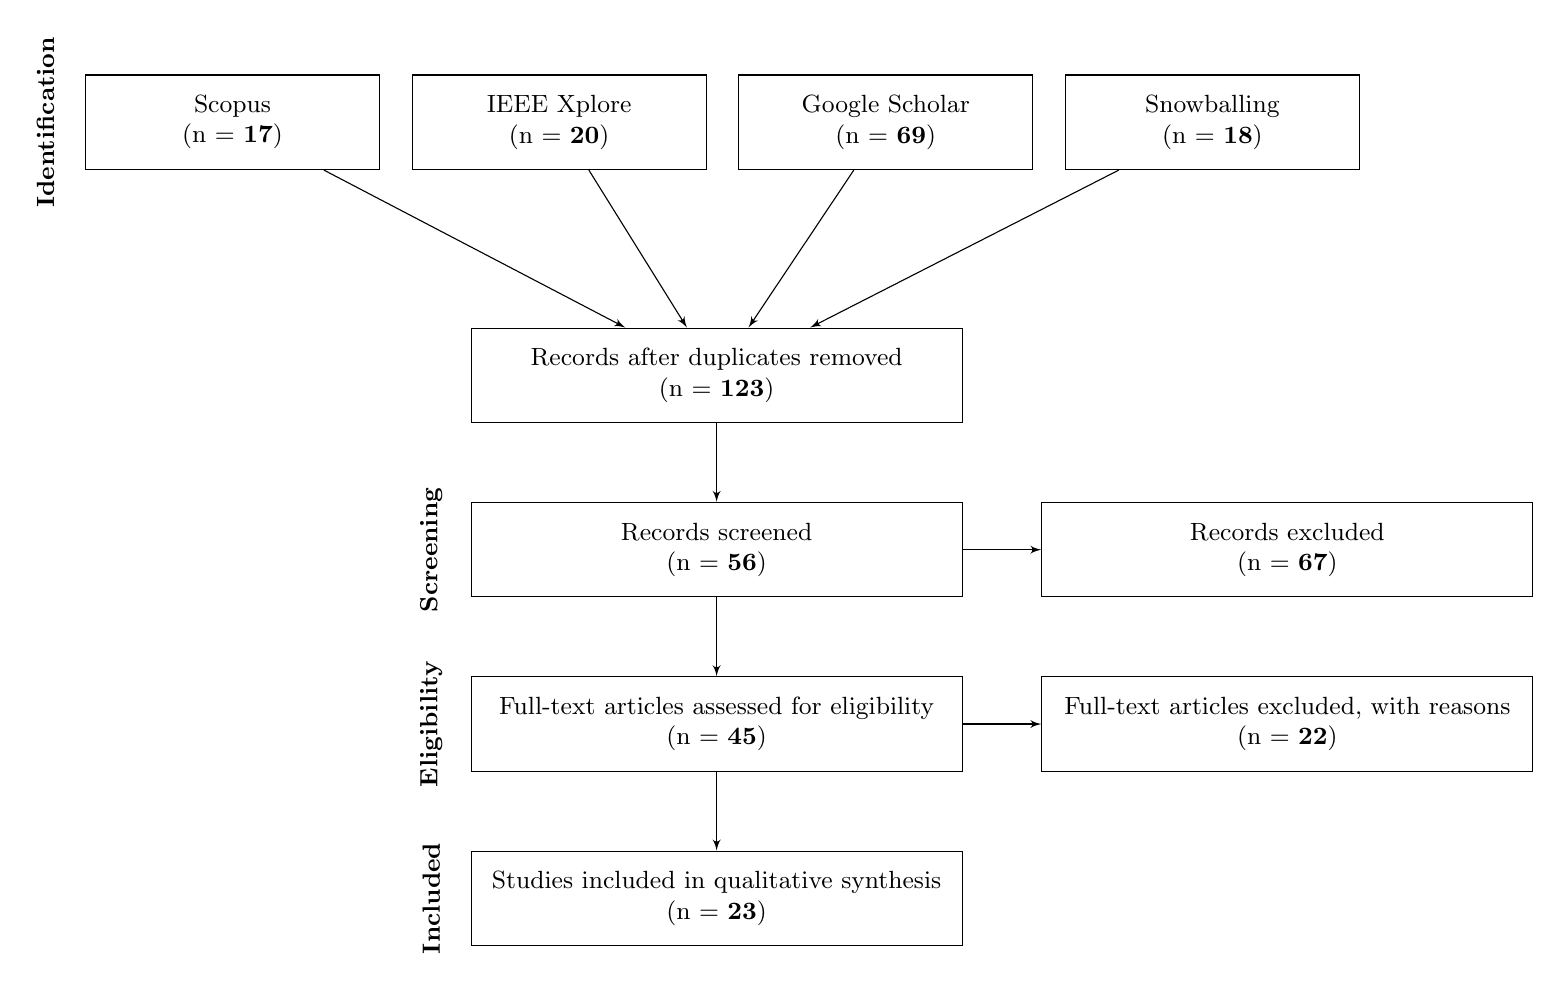
\begin{tikzpicture}[
    node distance=1.5cm,
    every node/.style={font=\small},
    block/.style={rectangle, draw, text width=6cm, align=center, minimum height=1.2cm},
    decision/.style={diamond, draw, text width=2cm, align=center, aspect=2},
    line/.style={draw, -latex'}
]

% Identification Phase
\node[block, text width=3.5cm] (scopus) {Scopus \\ (n = \textbf{17})};
\node[block, text width=3.5cm, right=0.4cm of scopus] (ieee) {IEEE Xplore \\ (n = \textbf{20})};
\node[block, text width=3.5cm, right=0.4cm of ieee] (scholar) {Google Scholar \\ (n = \textbf{69})};
\node[block, text width=3.5cm, right=0.4cm of scholar] (other) {Snowballing \\ (n = \textbf{18})};

% Screening Phase
\node[block, below=2cm of ieee, xshift=2cm] (duplicates) {Records after duplicates removed \\ (n = \textbf{123})};
\node[block, below=1cm of duplicates] (screened) {Records screened \\ (n = \textbf{56})};
\node[block, right=1cm of screened] (excluded) {Records excluded \\ (n = \textbf{67})};

% Eligibility Phase
\node[block, below=1cm of screened] (eligible) {Full-text articles assessed for eligibility \\ (n = \textbf{45})};
\node[block, right=1cm of eligible] (excluded_full) {Full-text articles excluded, with reasons \\ (n = \textbf{22})};

% Included Phase
\node[block, below=1cm of eligible] (included_qual) {Studies included in qualitative synthesis \\ (n = \textbf{23})};

% Connections
\path [line] (scopus) -- (duplicates);
\path [line] (ieee) -- (duplicates);
\path [line] (scholar) -- (duplicates);
\path [line] (other) -- (duplicates);
\path [line] (duplicates) -- (screened);
\path [line] (screened) -- (eligible);
\path [line] (screened) -- (excluded);
\path [line] (eligible) -- (included_qual);
\path [line] (eligible) -- (excluded_full);
% Removed connection to quantitative synthesis block

% Grouping labels (optional, can be added as nodes on the left)
\node[left=0.5cm of scopus, rotate=90, anchor=center] {\textbf{Identification}};
\node[left=0.5cm of screened, rotate=90, anchor=center] {\textbf{Screening}};
\node[left=0.5cm of eligible, rotate=90, anchor=center] {\textbf{Eligibility}};
\node[left=0.5cm of included_qual, rotate=90, anchor=center] {\textbf{Included}};

\end{tikzpicture}

	}
	\fcmfcaption{Schematic of the PRISMA selection process.}\label{rys:prisma}
\end{figure}

\paragraph{Inclusion Criteria.} The review will include papers that:
\begin{enumerate}
	\item Propose a method for \emph{automating} the training process (adaptive
	      curriculum or loss weighting).
	\item Address Multi-Task Learning challenges, specifically Negative Transfer or
	      parameter sharing.
	\item Utilize Meta-Learning, Self-Paced Learning, or Reinforcement Learning
	      approaches.
	\item Were published between 2017 and 2025.
\end{enumerate}

\paragraph{Data Extraction.} The following information will be extracted from selected papers:
\begin{itemize}
	\item \textbf{Metadata:} Title, year, publication venue.
	\item \textbf{Methodology:} Type of Curriculum (Static/Adaptive/SPL) and Optimization strategy.
	\item \textbf{Architecture:} Hard vs. Soft parameter sharing.
	\item \textbf{Results:} Mitigation of negative transfer and generalization improvements.
\end{itemize}

% Auto-generated archival appendix snippet for sweep-pack v1.
\chapter{Sweep Pack v1 Reproducibility Snapshot}
\label{app:sweep-pack-v1}

This appendix references the immutable archive in
\texttt{docs/results/2026-03-14\_sweep-pack-v1.md}.

\textbf{Run window:} 2026-03-14T15:15:21+01:00 to 2026-03-15T02:41:45+01:00.\\
\textbf{Source commit (pre-archive):} \texttt{bf8f54969c16dd7f16ee57e87313f20fb0f9c99c}.\\
\textbf{Trials:} 630 total, 336 finished, 294 pruned.

\begin{table}[h]
\centering
\small
\begin{tabular}{lrrll}
\toprule
Function & Best val loss & Median val loss & Best arch & Pruned \\
\midrule
franke\_n10000\_k5\_ss4\_seed42 & 2.526e-06 & 1.162e-05 & mlp & 41.2\% \\
friedman2\_2d\_n12000\_k6\_ss5\_seed42 & 3.901e-06 & 5.083e-05 & mlp & 48.9\% \\
friedman1\_2d\_n12000\_k5\_ss4p5\_seed42 & 1.078e-05 & 1.285e-04 & mlp & 40.0\% \\
peaks\_n10000\_k5\_ss5\_seed42 & 3.635e-05 & 3.945e-04 & siren & 51.2\% \\
bukin\_n10000\_k6\_ss8\_seed42 & 7.625e-05 & 7.444e-03 & mlp & 35.7\% \\
ackley\_n8000\_k5\_ss5\_seed42 & 2.024e-04 & 2.888e-01 & mlp & 50.0\% \\
levy\_n9000\_k5\_ss6\_seed42 & 6.195e-03 & 1.033e+00 & mlp & 57.1\% \\
eggholder\_n12000\_k6\_ss7\_seed42 & 6.023e+01 & 1.458e+03 & fourier & 48.9\% \\
\bottomrule
\end{tabular}
\caption{Best trial per function for sweep pack v1.}
\label{tab:sweep-pack-v1-best}
\end{table}

% Benchmark appendix with extended narrative and figures.
\chapter{Curriculum vs Single Benchmark v1}
\label{app:curr-vs-single-v1}

\section{Objective and motivation}

The core research question in this phase was:
\emph{Does curriculum training improve final quality, convergence behavior,
or efficiency relative to direct single-target training?}

This benchmark was designed as a controlled comparison where:

\begin{itemize}
    \item data generation settings were matched per function,
    \item hyperparameters were inherited from prior sweep best trials,
    \item only the training strategy changed (\texttt{single} vs \texttt{curriculum}).
\end{itemize}

The rationale was to evaluate whether curriculum contributes measurable value
beyond already-strong per-function hyperparameters.

\section{Experimental protocol}

\textbf{Benchmark id:} \texttt{curr\_vs\_single\_20260315\_175826}.\\
\textbf{Run window:} 2026-03-15T17:58:26+01:00 to 2026-03-16T01:10:36+01:00.\\
\textbf{Completed runs:} 96/96 (runner), 96/96 (MLflow FINISHED).

\paragraph{Factorial design.}

\begin{itemize}
    \item Methods: \texttt{single} vs \texttt{curriculum}
    \item Regimes: \texttt{equal\_epochs}, \texttt{equal\_time}
    \item Functions: 8 benchmark functions
    \item Seeds: 42, 43, 44
\end{itemize}

Total runs: \(2 \times 2 \times 8 \times 3 = 96\).

\paragraph{Primary metrics.}

\begin{itemize}
    \item final quality: \texttt{final\_hard\_val\_loss}
    \item efficiency: median runtime (seconds)
    \item secondary efficiency: time-to-target hit rate
\end{itemize}

In the delta tables, positive
\texttt{delta\_quality\_single\_minus\_curriculum} means curriculum has lower
(loss-better) median quality.

\section{Headline benchmark outcomes}

\begin{table}[h]
\centering
\small
\begin{tabular}{lrrrr}
\toprule
Regime & Quality (Curr.) & Quality (Single) & Runtime (Single) & Runtime (Curr.) \\
\midrule
equal\_epochs & 5 & 3 & 8 & 0 \\
equal\_time & 3 & 5 & 8 & 0 \\
\bottomrule
\end{tabular}
\caption{Win counts by regime.}
\label{tab:curr-vs-single-win-counts}
\end{table}

\begin{table}[h]
\centering
\small
\begin{tabular}{llll}
\toprule
Function & equal\_epochs & equal\_time & Runtime winner \\
\midrule
ackley & single & single & single \\
bukin & curriculum & curriculum & single \\
eggholder & single & single & single \\
franke & curriculum & curriculum & single \\
friedman1\_2d & curriculum & single & single \\
friedman2\_2d & curriculum & single & single \\
levy & curriculum & curriculum & single \\
peaks & single & single & single \\
\bottomrule
\end{tabular}
\caption{Quality winners by function and regime.}
\label{tab:curr-vs-single-function-winners}
\end{table}

\section{Visual diagnostics}

\begin{figure}[h]
    \centering
    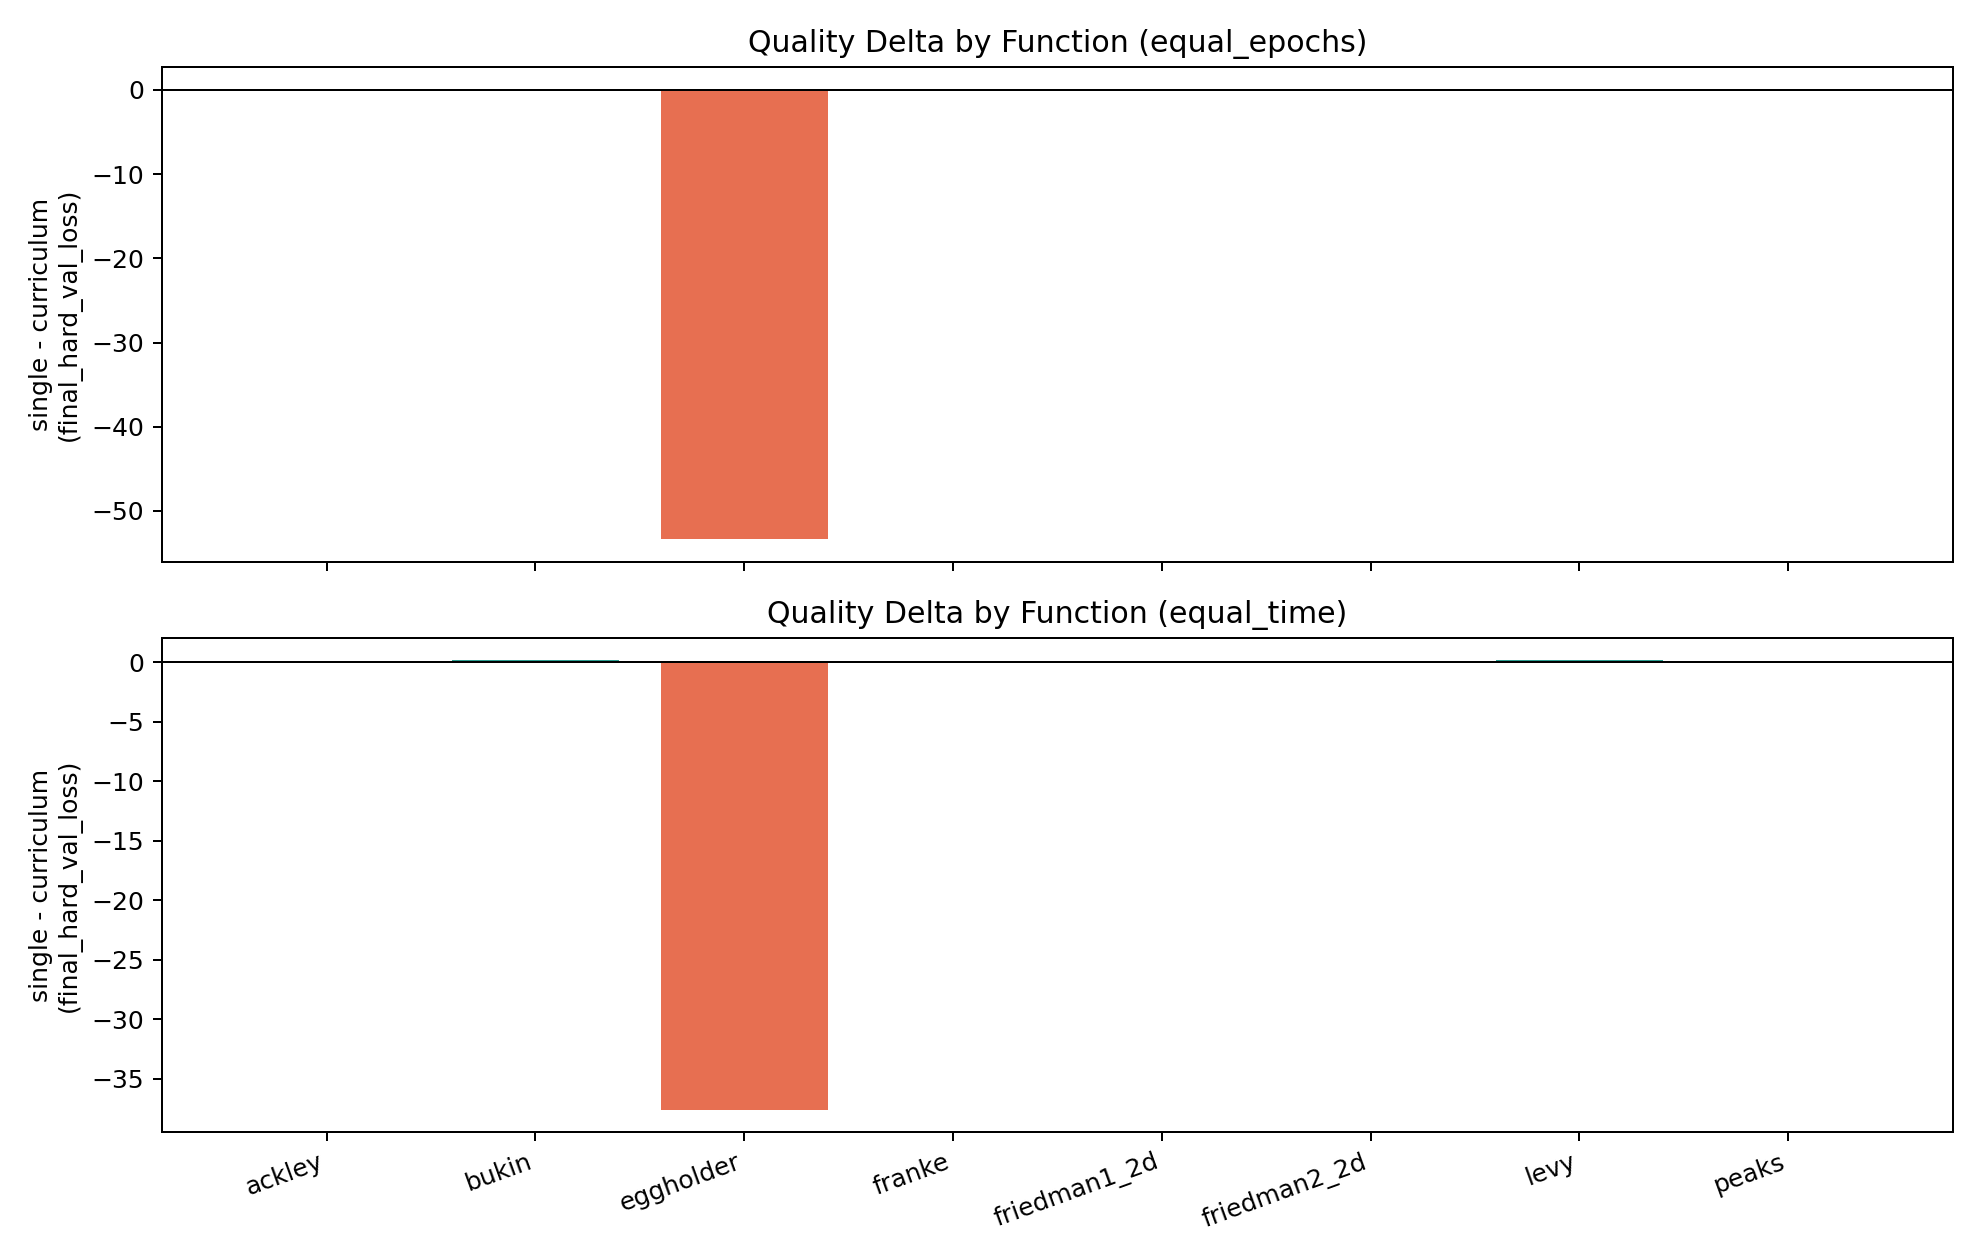
\includegraphics[width=0.95\textwidth]{figures/curr_vs_single_quality_delta.png}
    \caption{Quality delta per function (single minus curriculum). Positive bars favor curriculum.}
    \label{fig:curr-vs-single-quality-delta}
\end{figure}

\begin{figure}[h]
    \centering
    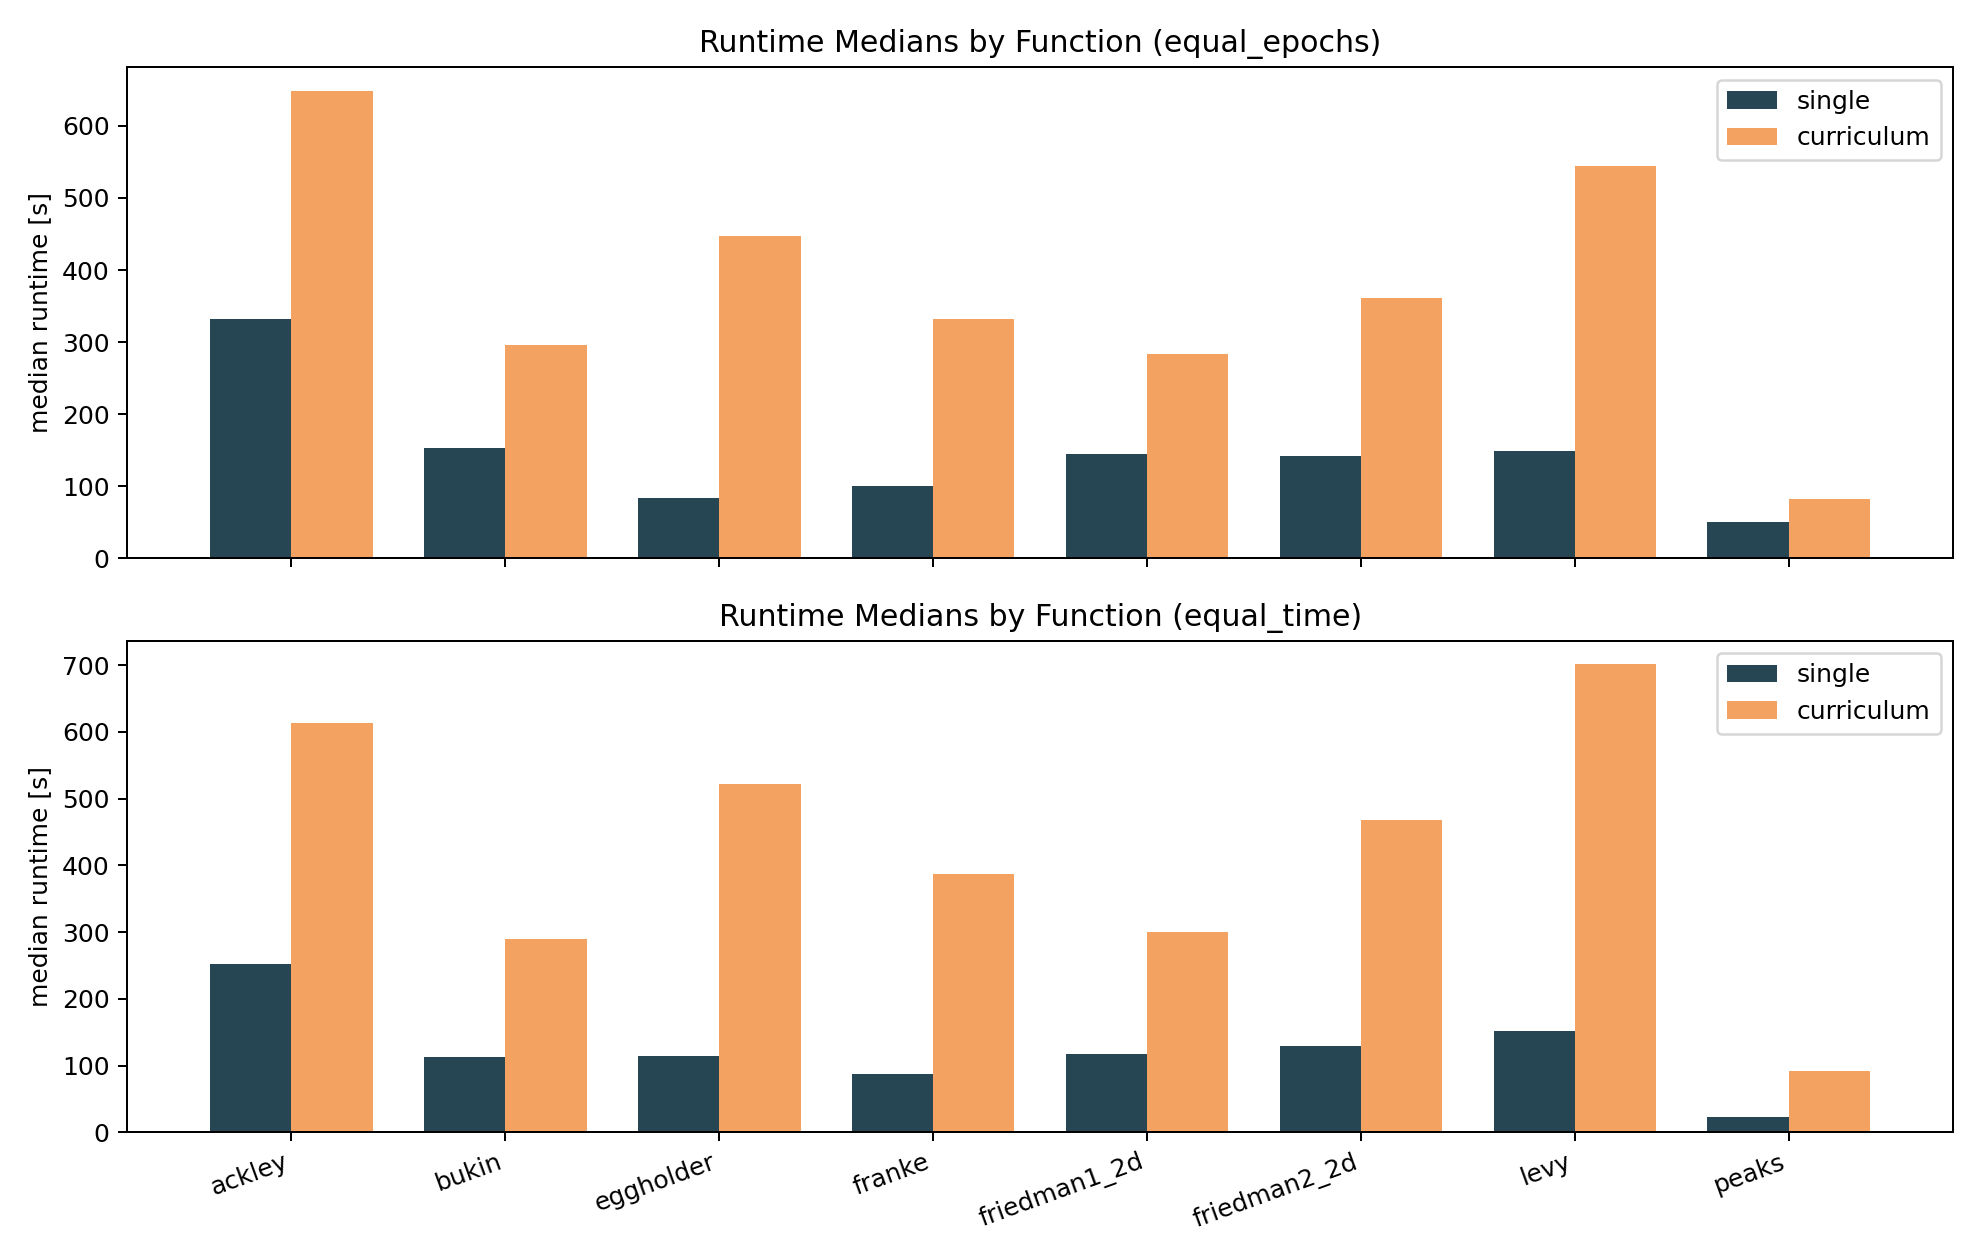
\includegraphics[width=0.95\textwidth]{figures/curr_vs_single_runtime_median.png}
    \caption{Median runtime by function and method for each regime.}
    \label{fig:curr-vs-single-runtime}
\end{figure}

\begin{figure}[h]
    \centering
    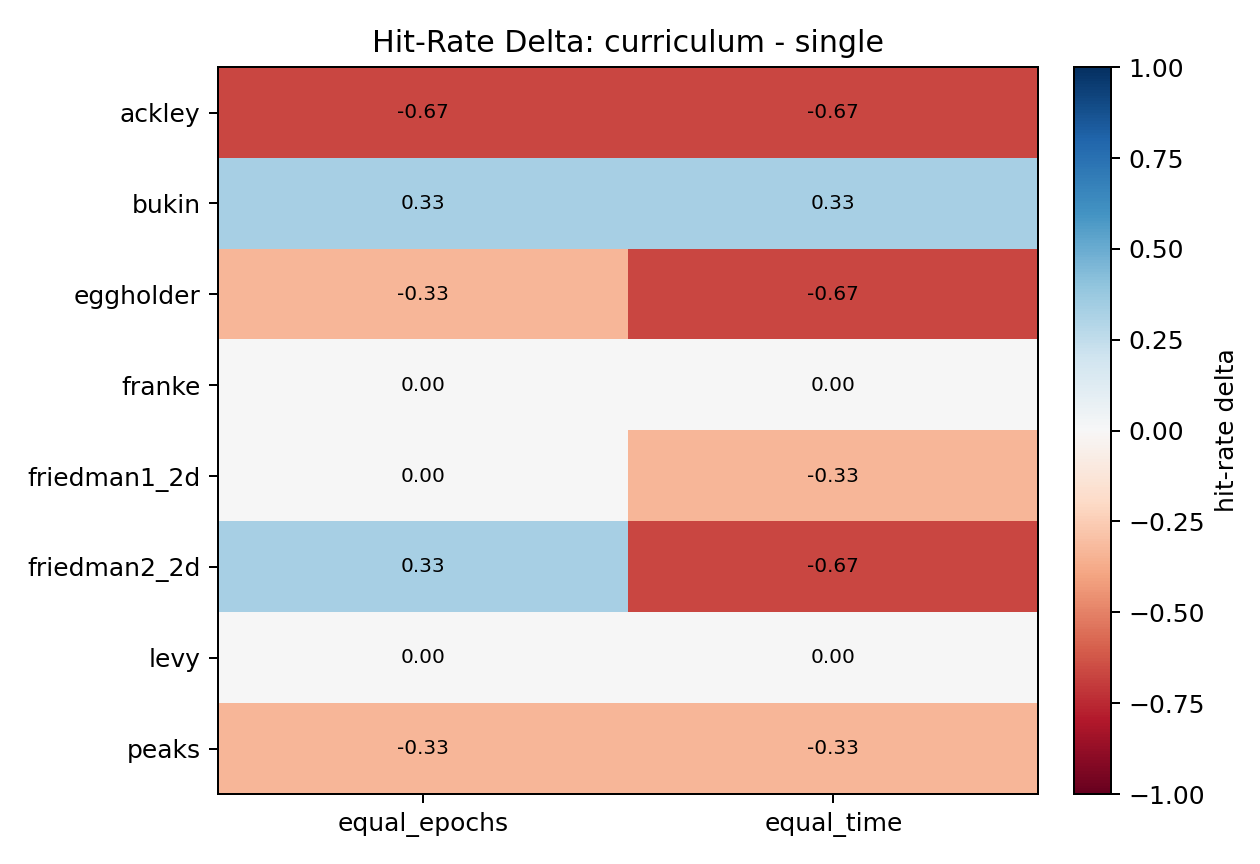
\includegraphics[width=0.72\textwidth]{figures/curr_vs_single_hitrate_delta.png}
    \caption{Time-to-target hit-rate delta (curriculum minus single). Negative values favor single.}
    \label{fig:curr-vs-single-hit-rate}
\end{figure}

\section{MLflow artifact inspection (learning dynamics)}

To inspect whether curriculum was practically useful beyond scalar summary
metrics, I additionally reviewed raw MLflow artifact plots from representative
runs (seed 42, equal\_epochs):

\begin{itemize}
    \item functions where curriculum helped quality: \texttt{bukin}, \texttt{levy},
    \item functions where curriculum did not help: \texttt{ackley}, \texttt{eggholder}.
\end{itemize}

The following figures are assembled directly from MLflow artifacts logged during
training (parent-run global metrics, child-run snapshots, and parent-run stage
surfaces).

\begin{figure}[h]
    \centering
    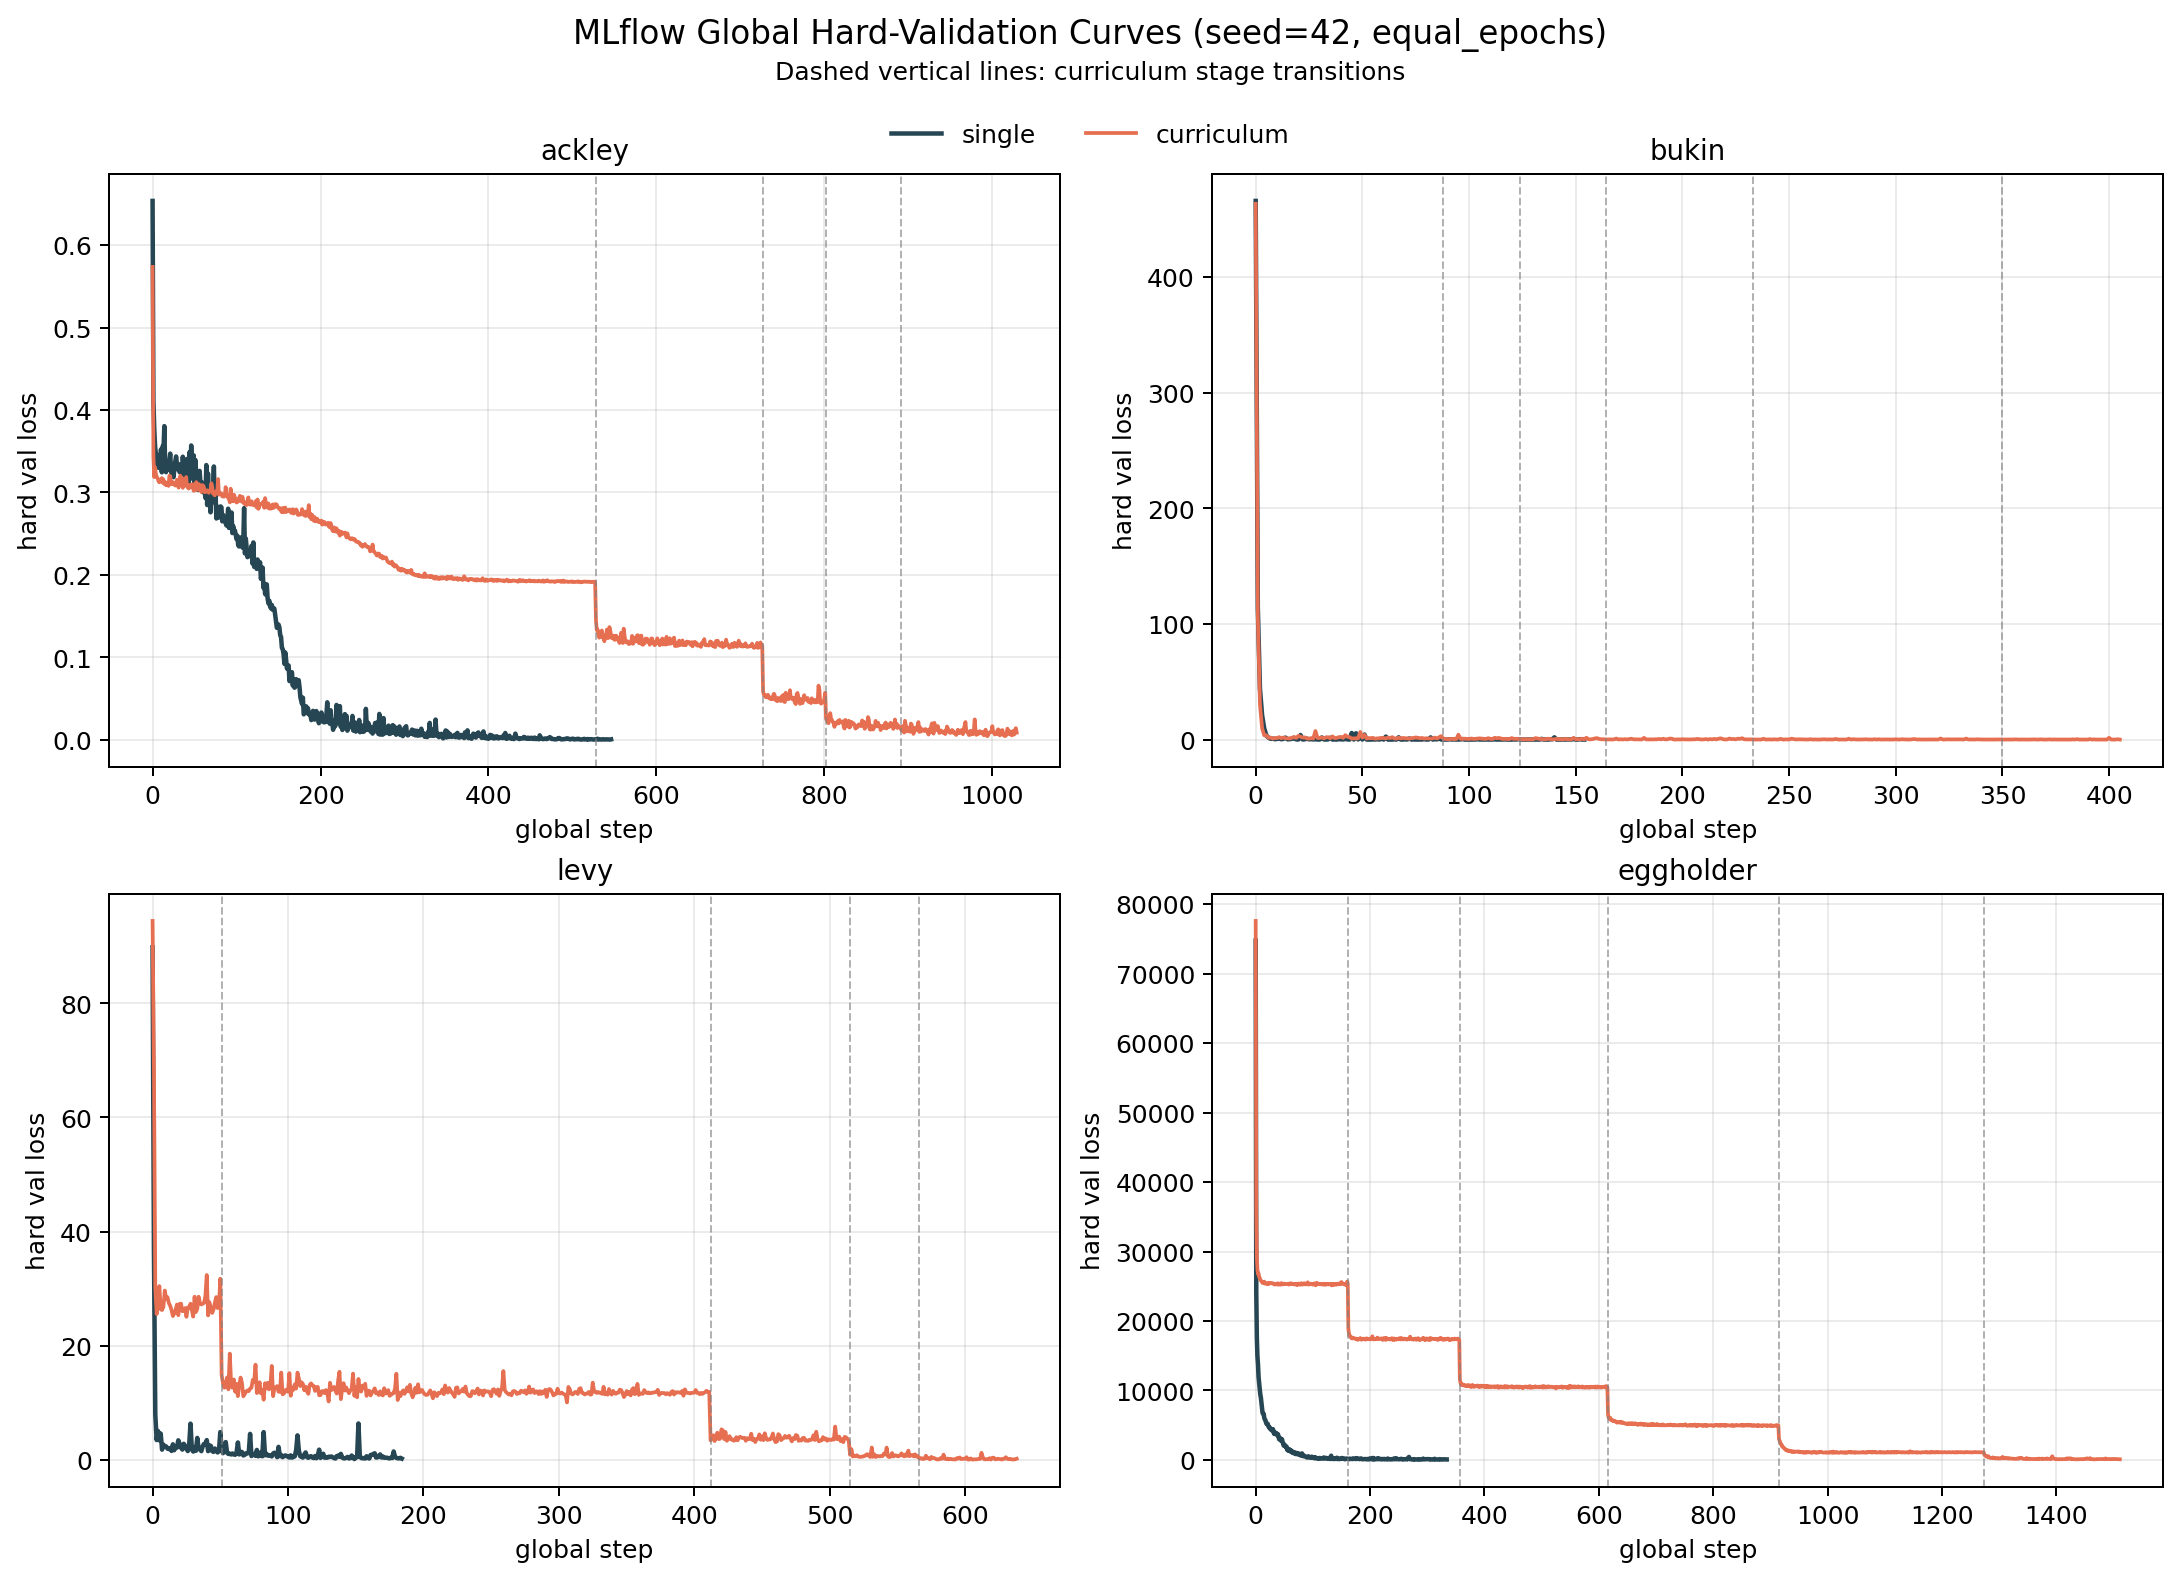
\includegraphics[width=0.98\textwidth]{figures/mlflow_curr_vs_single_global_hardval_seed42.png}
    \caption{MLflow parent-run global hard-validation curves (single vs curriculum). Dashed vertical lines mark curriculum stage transitions.}
    \label{fig:mlflow-learning-curves}
\end{figure}

\begin{figure}[h]
    \centering
    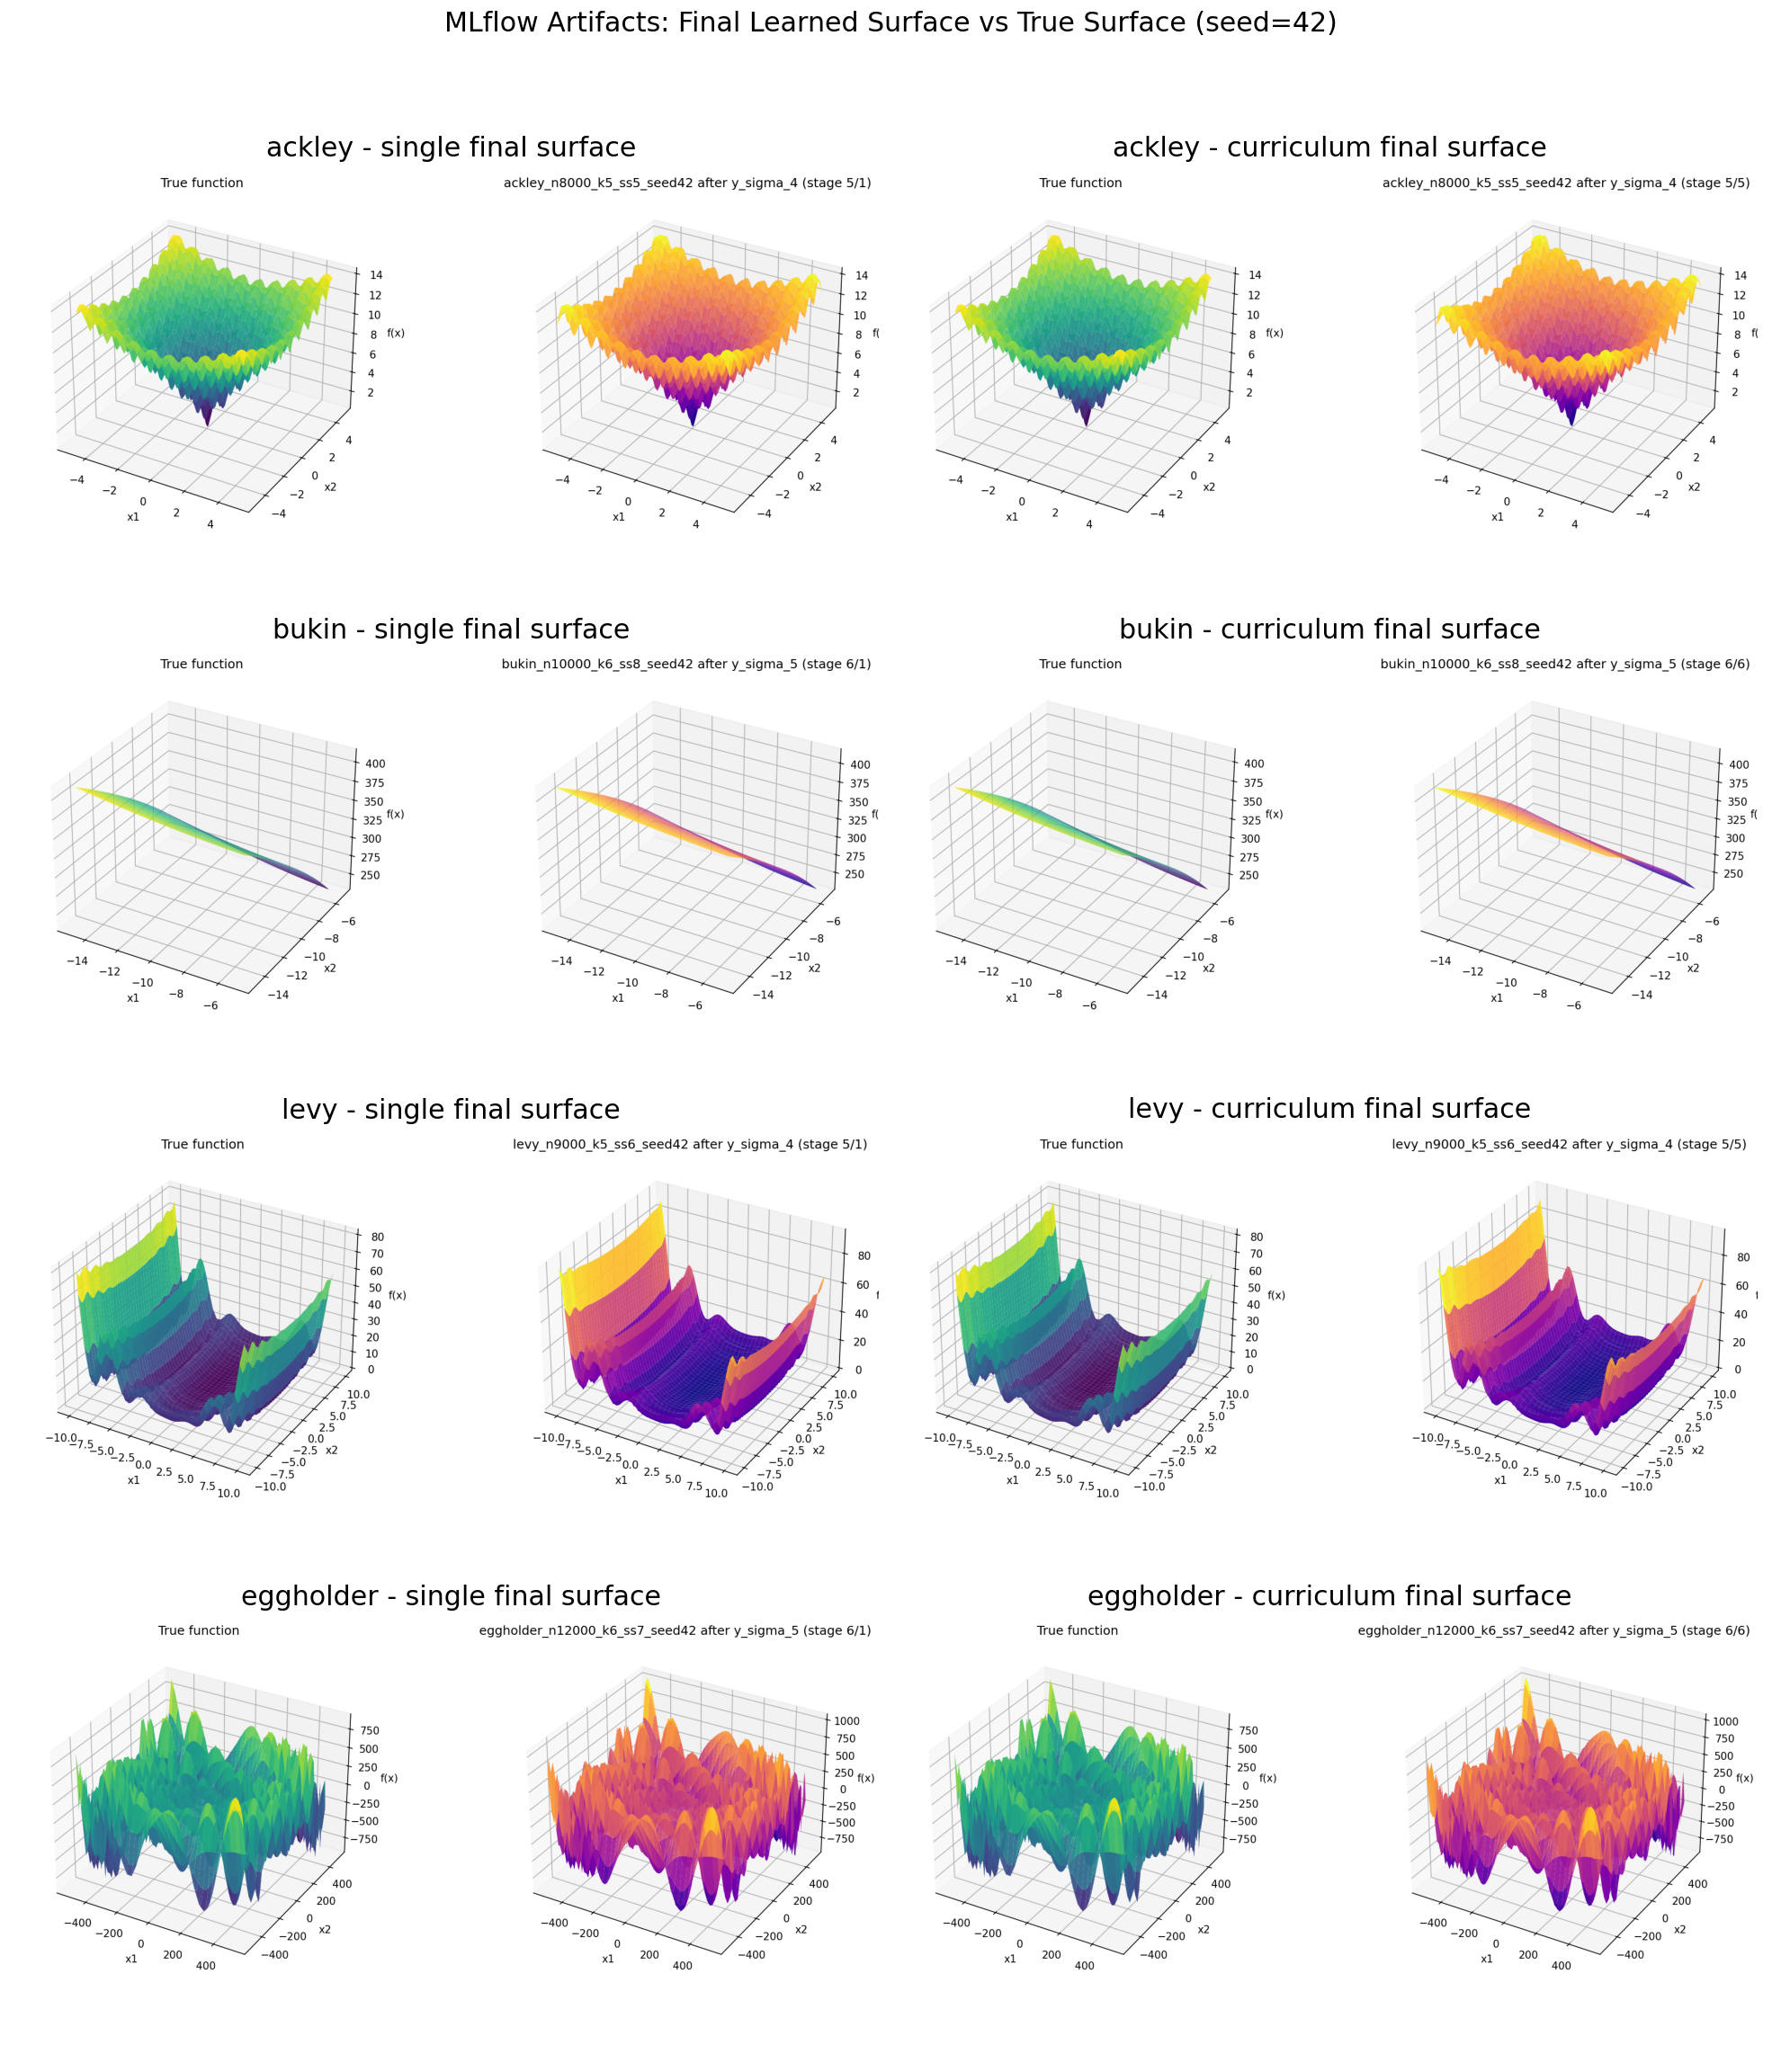
\includegraphics[width=0.98\textwidth]{figures/mlflow_curr_vs_single_final_surfaces_seed42.png}
    \caption{Final learned surfaces from MLflow artifacts. Each panel includes the learned surface and reference true surface used in training diagnostics.}
    \label{fig:mlflow-final-surfaces}
\end{figure}

\begin{figure}[h]
    \centering
    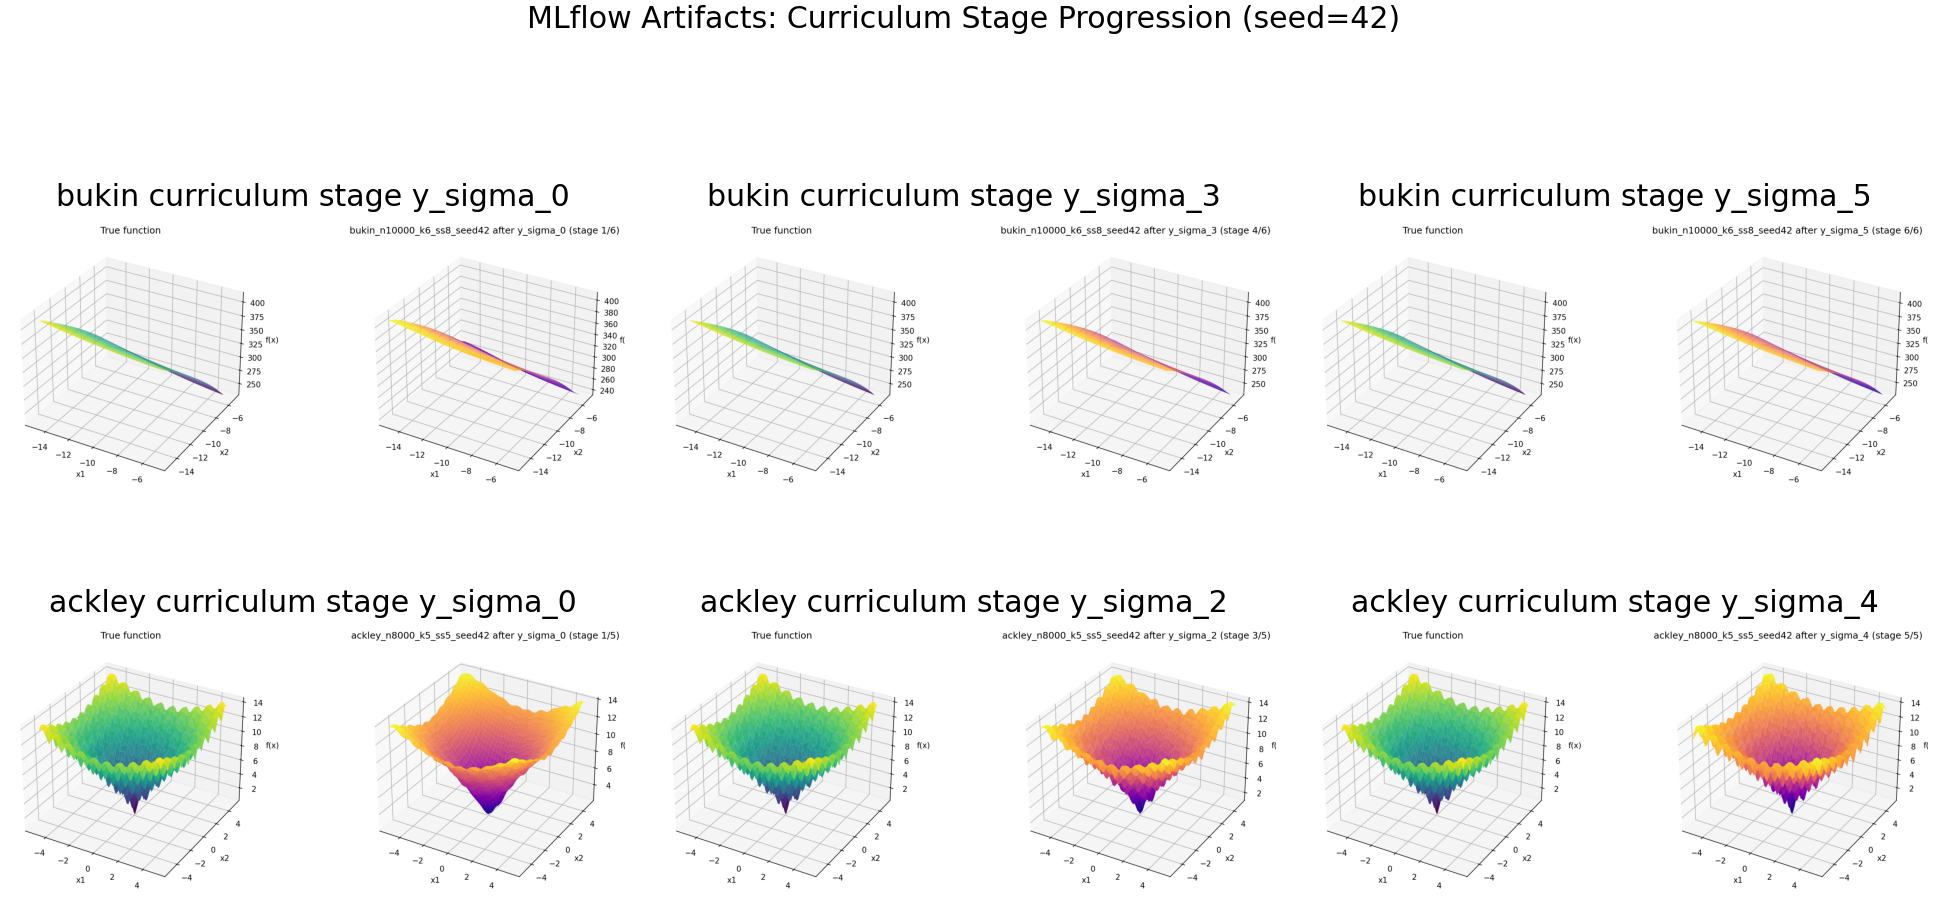
\includegraphics[width=0.98\textwidth]{figures/mlflow_curriculum_stage_progression_seed42.png}
    \caption{Curriculum stage progression for two representative functions (early, middle, final sigma stages).}
    \label{fig:mlflow-curriculum-stage}
\end{figure}

\begin{figure}[h]
    \centering
    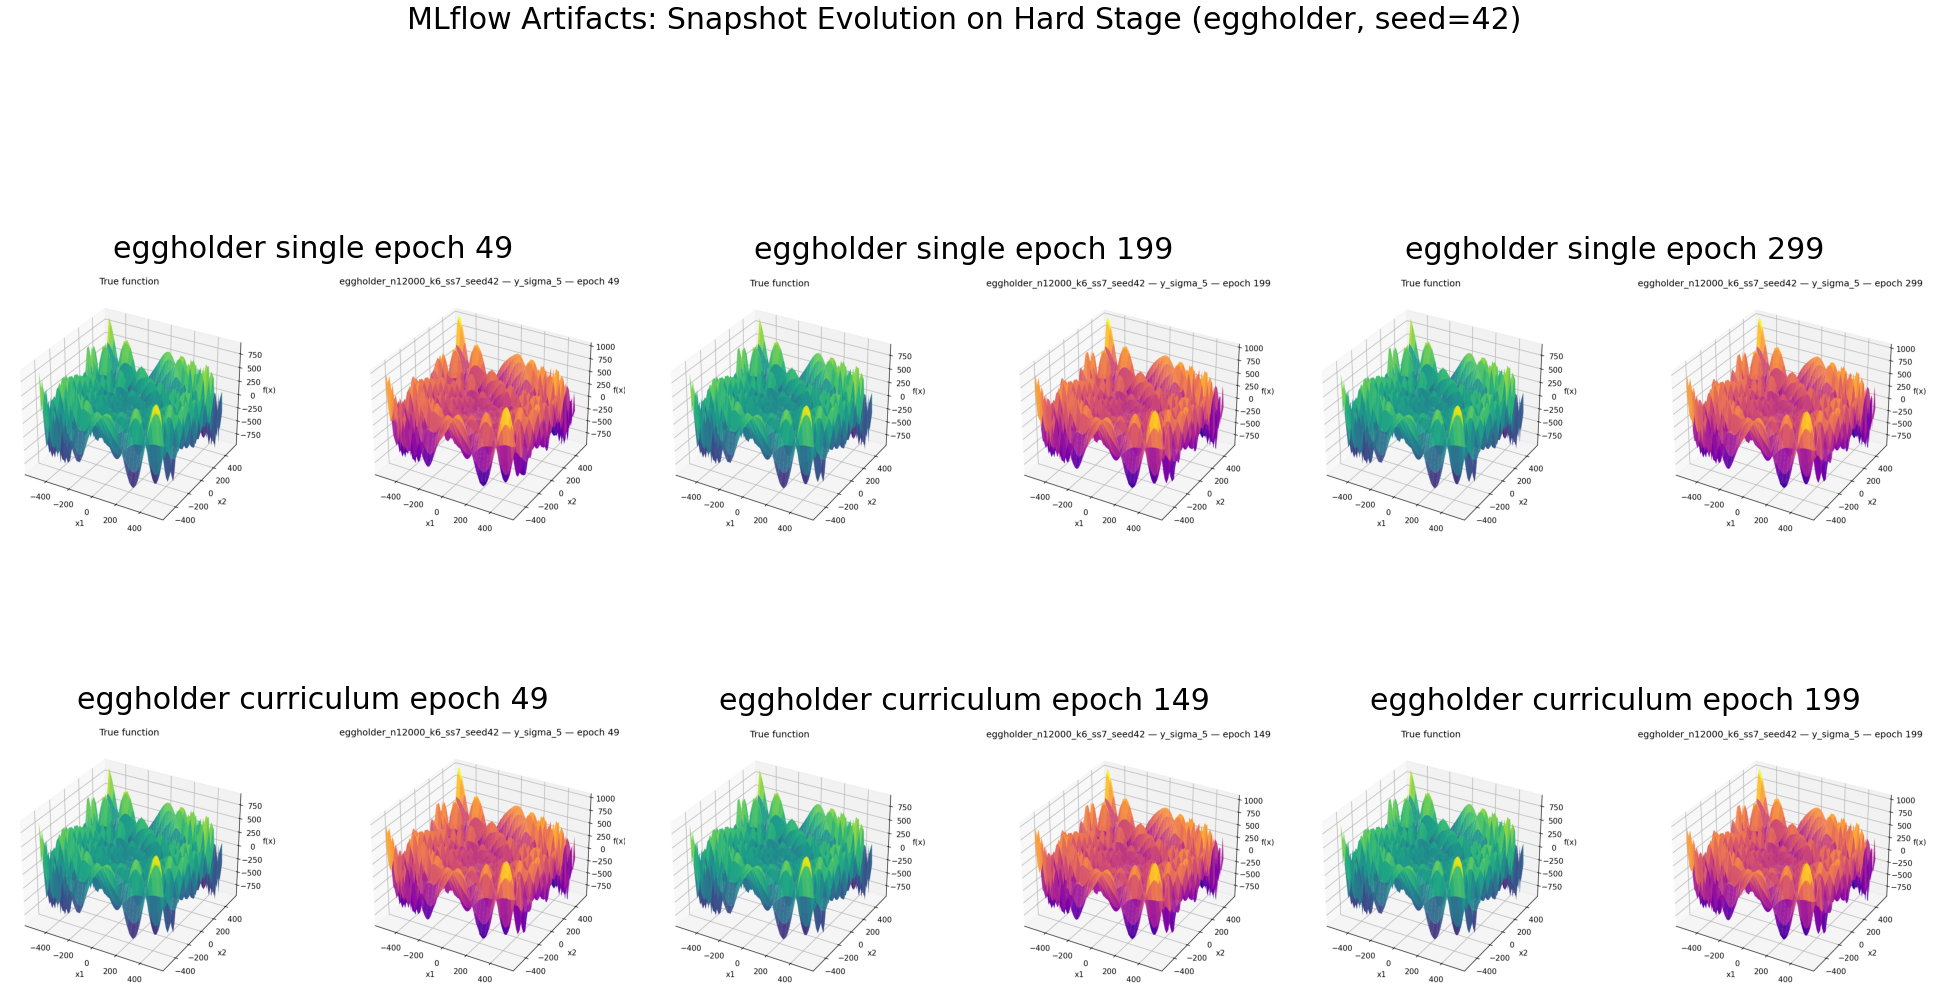
\includegraphics[width=0.98\textwidth]{figures/mlflow_eggholder_snapshot_evolution_seed42.png}
    \caption{Snapshot evolution on the hard stage for \texttt{eggholder} (single vs curriculum).}
    \label{fig:mlflow-eggholder-snapshots}
\end{figure}

\paragraph{What these artifact plots show.}
\begin{itemize}
    \item Curriculum often reaches smoother intermediate surfaces, but this comes
          with substantial extra compute time per run.
    \item For functions such as \texttt{bukin} and \texttt{levy}, curriculum trajectories
          can end closer to the target surface than single training.
    \item For \texttt{ackley} and \texttt{eggholder}, additional curriculum stages do
          not consistently translate into better hard-target final quality.
\end{itemize}

\section{Interpretation}

\paragraph{What worked.}
Curriculum provided repeatable quality gains for selected functions
(especially \texttt{bukin}, \texttt{franke}, and \texttt{levy}), indicating that
progressive smoothing can help optimization in some landscapes.

\paragraph{What did not work.}
Runtime increased in every function/regime cell.
In this benchmark, curriculum never won on runtime.

\paragraph{What this means.}
Curriculum should not be treated as a universal default. The current evidence
supports a selective policy:

\begin{itemize}
    \item use curriculum where quality gains are consistent,
    \item keep single-target training as the default baseline elsewhere,
    \item optimize curriculum schedule depth only where it materially helps.
\end{itemize}

\section{Limitations and next actions}

\begin{itemize}
    \item The \texttt{equal\_time} regime used a relatively high timeout cap,
          so it often did not enforce a tight budget.
    \item A stricter per-function cap (near single median runtime) should be used
          in the next iteration for stronger efficiency conclusions.
    \item The next cycle should test reduced-stage curriculum variants to lower runtime
          overhead while preserving gains on functions where curriculum helps.
\end{itemize}

\section{Strategic conclusion after two experiments}

After completing both stages reported in this thesis appendix
(the sweep-pack baseline and the curriculum-vs-single benchmark),
I conclude that the current baseline model capacity is too high to serve as a
useful foundation for curriculum-learning analysis. In practice, the baseline
single-target model often converges too strongly, leaving limited room for
curriculum to demonstrate consistent gains.

Therefore, the next research phase should focus on re-establishing a better
operating point before further curriculum claims are made.

\paragraph{Planned next phase.}
\begin{enumerate}
    \item \textbf{Capacity--data study:} determine an appropriate relation between
          dataset size and model parameter count for each function family.
    \item \textbf{Controlled re-sweep:} rerun hyperparameter sweeps under reduced
          model capacities and validated dataset sizes.
    \item \textbf{Training-loop refactor:} use this rerun to simplify and harden the
          experiment loop for cleaner reproducibility and easier ablation control.
    \item \textbf{Richer MLflow instrumentation:} log more detailed optimization
          diagnostics beyond losses, including roughness-related proxies
          (e.g., gradient variance, gradient-norm statistics, curvature/Hessian
          approximations, and stage-to-stage stability indicators).
    \item \textbf{Literature grounding first:} before implementation, conduct a short
          focused review on (a) parameter-count selection for regression settings
          and (b) quantitative loss-landscape roughness metrics.
\end{enumerate}

This plan is intended to produce a more informative baseline where curriculum
effects, if present, can be measured more reliably and interpreted with higher
confidence.

% Appendix draft for the current v3 ratio-constrained noisy sweep.
\chapter{Sweep Pack v3: Experiment Setting (Draft)}
\label{app:sweep-pack-v3-setup}

\section{Purpose of this experiment}

This experiment defines a stronger baseline for later curriculum-learning
evaluation by using:
\begin{itemize}
    \item fixed data volume and split policy across all functions,
    \item controlled observation noise in training data generation,
    \item explicit parameter-to-training-samples constraints,
    \item expanded optimization diagnostics logged to MLflow.
\end{itemize}

The objective is to establish a reproducible and non-trivial optimization setup
before comparing curriculum strategies.

\section{Dataset construction protocol}

For each benchmark function, data are generated from the analytical function and
saved as two separate files:
\begin{itemize}
    \item \texttt{*\_train.parquet}: used for model fitting and internal train/val split,
    \item \texttt{*\_test.parquet}: used only for final holdout evaluation.
\end{itemize}

\paragraph{Current default settings (v3).}
\begin{itemize}
    \item Total generated samples per function: \texttt{20000}
    \item Holdout policy: \texttt{10000 train file + 10000 test file}
    \item Internal split inside train file: \texttt{80/20} (effective \texttt{8000/2000})
    \item Number of smoothing levels: \texttt{3}
    \item Noise model: additive Gaussian label noise
    \item Noise ratio: \texttt{0.03} (relative to target standard deviation)
    \item Random seed: \texttt{42}
\end{itemize}

\section{Sweep protocol and search constraints}

\paragraph{Runner.}
The sweep pack is executed with:
\begin{verbatim}
./scripts/run_sweep_pack_v3_ratio.sh
\end{verbatim}

\paragraph{Functions included.}
\texttt{ackley, levy, bukin, eggholder, franke, peaks, friedman1\_2d, friedman2\_2d}.

\paragraph{Per-function study settings.}
\begin{itemize}
    \item Trials per function: \texttt{90}
    \item Architectures searched: \texttt{MLP, SIREN, Fourier}
    \item Early stopping patience: \texttt{25}
    \item Ratio constraint: \(\texttt{train\_samples} / \texttt{n\_params} \in [5, 10]\)
\end{itemize}

Because training uses the internal train split (\(\approx 8000\) samples), the
effective valid parameter range is approximately:
\[
    \texttt{n\_params} \in [800, 1600].
\]

\section{Metrics logged to MLflow}

\paragraph{Primary quality metrics.}
\begin{itemize}
    \item \texttt{best\_val\_loss}
    \item \texttt{final\_hard\_val\_loss}
    \item \texttt{final\_test\_loss} (from \texttt{*\_test.parquet})
\end{itemize}

\paragraph{Optimization-stability diagnostics (new).}
\begin{itemize}
    \item Step-wise: \texttt{grad\_cosine\_sim}, \texttt{grad\_variance},
          \texttt{grad\_noise\_scale}, \texttt{gsnr}
    \item Epoch-wise: \texttt{hessian\_trace}, \texttt{critical\_sharpness},
          \texttt{weight\_alpha} and layer-wise \texttt{weight\_alpha\_<layer>}
\end{itemize}

\subsection{Interpretation of roughness and stability metrics}

This subsection explains how each diagnostic should be interpreted when
presenting results.

\paragraph{1) Gradient cosine similarity (\texttt{grad\_cosine\_sim}, step-wise).}
For consecutive minibatch gradients \(g_t\) and \(g_{t-1}\), we compute:
\[
\cos(g_t, g_{t-1}) = \frac{g_t^\top g_{t-1}}{\|g_t\|\|g_{t-1}\|}.
\]
\begin{itemize}
    \item Values near \(1\): successive updates point in similar directions (stable descent).
    \item Values near \(0\): weak directional agreement (noisy/random-walk behavior).
    \item Negative values: oscillation or bouncing between opposite directions.
\end{itemize}

\paragraph{2) Gradient variance (\texttt{grad\_variance}, step-wise).}
This is the variance of gradient components at a given optimization step.
\begin{itemize}
    \item Low variance: cleaner optimization signal.
    \item High variance: stronger stochastic noise in updates.
\end{itemize}
Large spikes often indicate unstable regions or difficult minibatches.

\paragraph{3) Gradient noise scale (\texttt{grad\_noise\_scale}, step-wise).}
This is an EMA-based proxy of gradient variance across steps (smoothed noise level).
\begin{itemize}
    \item Decreasing trend: training becomes more stable.
    \item Persistently high values: optimization remains noise-dominated.
\end{itemize}

\paragraph{4) Gradient signal-to-noise ratio (\texttt{gsnr}, step-wise).}
Computed as:
\[
\mathrm{GSNR} = \frac{(\mathrm{E}[g])^2}{\mathrm{Var}(g)}.
\]
\begin{itemize}
    \item Higher GSNR: learning signal dominates gradient noise.
    \item Lower GSNR: updates are mostly stochastic noise.
\end{itemize}
GSNR is useful for identifying noise-limited training phases.

\paragraph{5) Hutchinson Hessian trace (\texttt{hessian\_trace}, epoch-wise).}
The Hessian \(H\) captures local curvature of the loss surface. Its trace
\(\mathrm{tr}(H)\) is estimated using a random Rademacher probe \(v\):
\[
\mathrm{tr}(H) \approx v^\top H v.
\]
\begin{itemize}
    \item Higher trace: sharper local curvature.
    \item Lower trace: flatter local geometry.
\end{itemize}
This metric provides a direct proxy of local loss-landscape roughness.

\paragraph{6) Critical sharpness (\texttt{critical\_sharpness}, epoch-wise).}
This approximates the critical step size \(\eta_c\) along the update direction
at which loss starts to increase (estimated by short binary search).
\begin{itemize}
    \item Larger \(\eta_c\): wider stability margin.
    \item Smaller \(\eta_c\): near edge-of-stability regime.
\end{itemize}
In practice, a very small \(\eta_c\) indicates sensitivity to learning-rate
perturbations.

\paragraph{7) Spectral alpha (\texttt{weight\_alpha}, epoch-wise).}
For each weight matrix, singular values are fitted with a power-law slope
exponent \(\alpha\). The run logs:
\begin{itemize}
    \item global mean \texttt{weight\_alpha},
    \item per-layer values \texttt{weight\_alpha\_<layer>}.
\end{itemize}
Typical interpretation:
\begin{itemize}
    \item stable moderate \(\alpha\): more regularized representation regime,
    \item erratic/extreme \(\alpha\): potential representational instability.
\end{itemize}

\paragraph{How to read them together.}
The metrics are complementary:
\begin{itemize}
    \item Directional stability: \texttt{grad\_cosine\_sim}
    \item Stochasticity level: \texttt{grad\_variance}, \texttt{grad\_noise\_scale}, \texttt{gsnr}
    \item Local geometry: \texttt{hessian\_trace}, \texttt{critical\_sharpness}
    \item Representation structure: \texttt{weight\_alpha}
\end{itemize}
This combination allows diagnosing not only final quality but also \emph{how}
the optimizer traverses the landscape during training.

\paragraph{Traceability and reproducibility.}
Each run logs:
\begin{itemize}
    \item full run configuration as artifact,
    \item dataset artifacts used by the run (\texttt{train} and \texttt{test}),
    \item Optuna trial metadata and pruning status.
\end{itemize}

\section{Status note}

This chapter documents the experimental \emph{setting} only. Detailed numerical
results, comparative interpretation, and ablation conclusions will be added in a
later revision once all v3 studies are complete and analyzed.

% Appendix for eggholder meta-weighting benchmark (unroll=1 only).
\chapter{Meta-weighting benchmark on \texttt{eggholder} (unroll = 1)}
\label{app:meta-weighting-eggholder-u1}

\section{Purpose and scope}

This appendix summarizes the reduced meta-weighting benchmark executed after the
longer differentiable unroll variants (\texttt{meta\_unroll\_steps}=3,5)
showed frequent optimization divergence. To obtain a stable comparison set, the
benchmark was rerun with \texttt{meta\_unroll\_steps}=1 only.

The objective of this experiment was to test whether adaptive gradient-based
loss weighting over Gaussian-continuation targets can improve the final hard
validation loss on the \texttt{eggholder} surface, and under which learning-rate
and noise settings this happens.

\section{Experimental protocol}

\textbf{Benchmark id:} \texttt{meta\_weighting\_eggholder\_u1\_20260504\_221357}.\\
\textbf{Function:} \texttt{eggholder}.\\
\textbf{Completed runs:} 288/288.\\
\textbf{Failed runs:} 0/288.\\
\textbf{Meta lookahead:} \texttt{meta\_unroll\_steps}=1.

\paragraph{Factorial design.}
\begin{itemize}
    \item Numbers of losses: \texttt{1, 2, 3, 5}
    \item Model learning rates: \texttt{0.01, 0.03}
    \item Meta learning rates: \texttt{0.0003, 0.001, 0.003}
    \item Noise ratios: \texttt{0.0, 0.05, 0.2}
    \item Seeds: \texttt{42, 666, 777, 888}
\end{itemize}

Total runs:
\[
4 \times 2 \times 3 \times 3 \times 4 = 288.
\]

\paragraph{Primary metric.}
The main comparison metric is the final hard validation loss
(\texttt{final\_val\_loss}); lower values are better.

\section{Headline results}

\begin{table}[h]
\centering
\small
\begin{tabular}{lrrrr}
\toprule
Losses & Runs & Mean final val loss & Median final val loss & Mean rank \\
\midrule
1 & 72 & 80650.90 & 82870.60 & 2.35 \\
2 & 72 & 81910.62 & 84069.00 & 2.50 \\
3 & 72 & 80974.89 & 82975.01 & 2.43 \\
5 & 72 & 82428.87 & 84139.55 & 2.72 \\
\bottomrule
\end{tabular}
\caption{Aggregate performance by number of weighted losses. Lower validation loss and lower rank are better.}
\label{tab:meta-eggholder-u1-by-losses}
\end{table}

\begin{table}[h]
\centering
\small
\begin{tabular}{lrrr}
\toprule
Losses & Mean improvement vs baseline & Median improvement vs baseline & Fraction improved vs baseline \\
\midrule
2 & -1259.72 & -1089.23 & 0.458 \\
3 &  -324.00 &  -549.98 & 0.472 \\
5 & -1777.98 & -1305.75 & 0.417 \\
\bottomrule
\end{tabular}
\caption{Paired comparison against the baseline \texttt{num\_losses=1}. Positive improvement means that adaptive weighting improves over the baseline; in this experiment all means remain negative.}
\label{tab:meta-eggholder-u1-vs-baseline}
\end{table}

\paragraph{Main takeaway.}
On average, the single-loss baseline (hard-target-only, \texttt{num\_losses=1})
remains the strongest setting in this benchmark. Among the adaptive variants,
\texttt{num\_losses=3} is the closest to the baseline on average, while
\texttt{num\_losses=5} is the weakest overall.

\section{Best observed configurations}

\begin{table}[h]
\centering
\small
\begin{tabular}{lrrrrr}
\toprule
Losses & Noise & $\eta_{\mathrm{model}}$ & $\eta_{\mathrm{meta}}$ & Median final val loss & Mean rank \\
\midrule
1 & 0.00 & 0.03 & 0.0003 & 62717.65 & 1.50 \\
3 & 0.00 & 0.03 & 0.0010 & 69440.03 & 1.75 \\
5 & 0.05 & 0.03 & 0.0030 & 73375.20 & 2.25 \\
3 & 0.05 & 0.03 & 0.0030 & 75490.82 & 2.00 \\
2 & 0.20 & 0.03 & 0.0030 & 75883.22 & 1.75 \\
\bottomrule
\end{tabular}
\caption{Best aggregate settings (sorted approximately by median final validation loss).}
\label{tab:meta-eggholder-u1-best-settings}
\end{table}

The best \emph{single run} in the full matrix was:
\begin{quote}
\texttt{num\_losses=2}, noise ratio \texttt{0.05},
$\eta_{\mathrm{model}}=0.03$, $\eta_{\mathrm{meta}}=0.003$,
seed \texttt{42}, with final validation loss \texttt{52323.09}.
\end{quote}

This means that adaptive weighting can occasionally produce very strong
individual runs, but this advantage was not stable enough across seeds and
conditions to outperform the single-loss baseline on average.

\section{Aggregate visual diagnostics}

\begin{figure}[h]
    \centering
    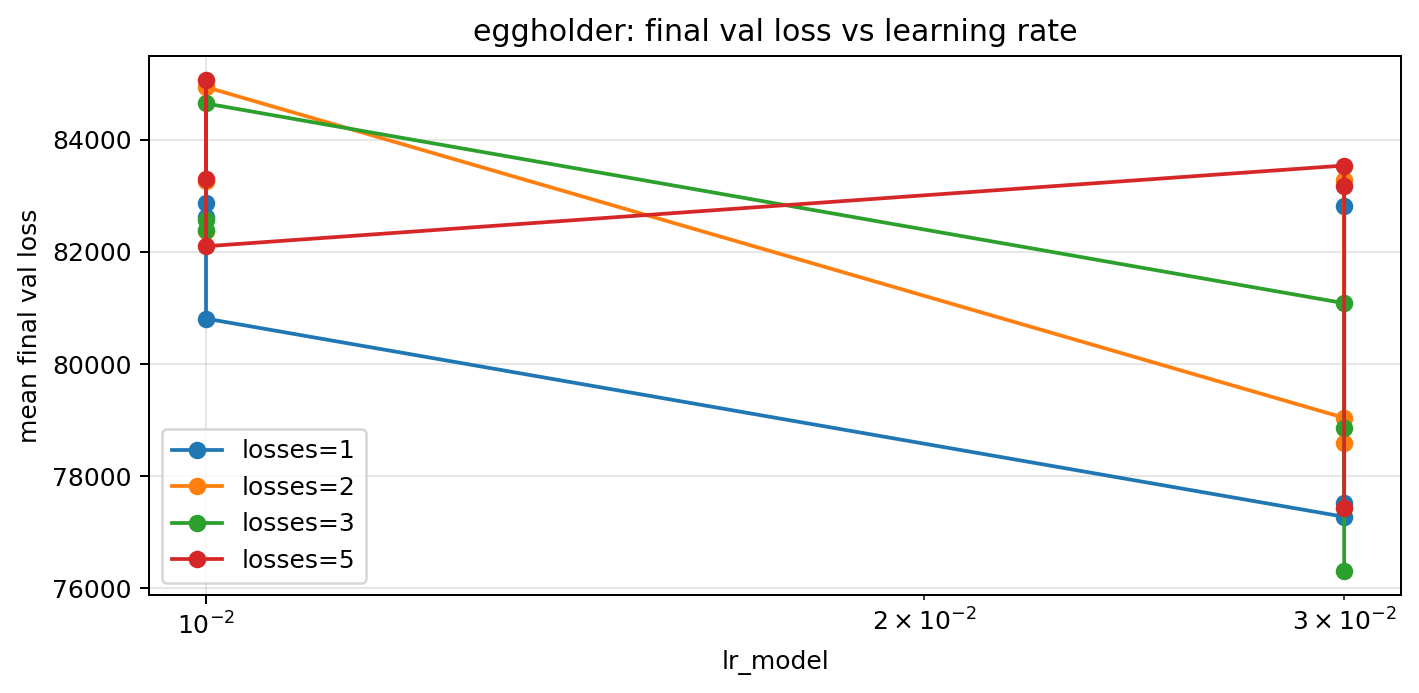
\includegraphics[width=0.92\textwidth]{figures/meta_weighting_eggholder_u1_final_val_loss_vs_lr.png}
    \caption{Mean final validation loss as a function of model learning rate, separated by the number of losses. The higher model learning rate (0.03) is frequently competitive or better than 0.01.}
    \label{fig:meta-eggholder-u1-vs-lr}
\end{figure}

\begin{figure}[h]
    \centering
    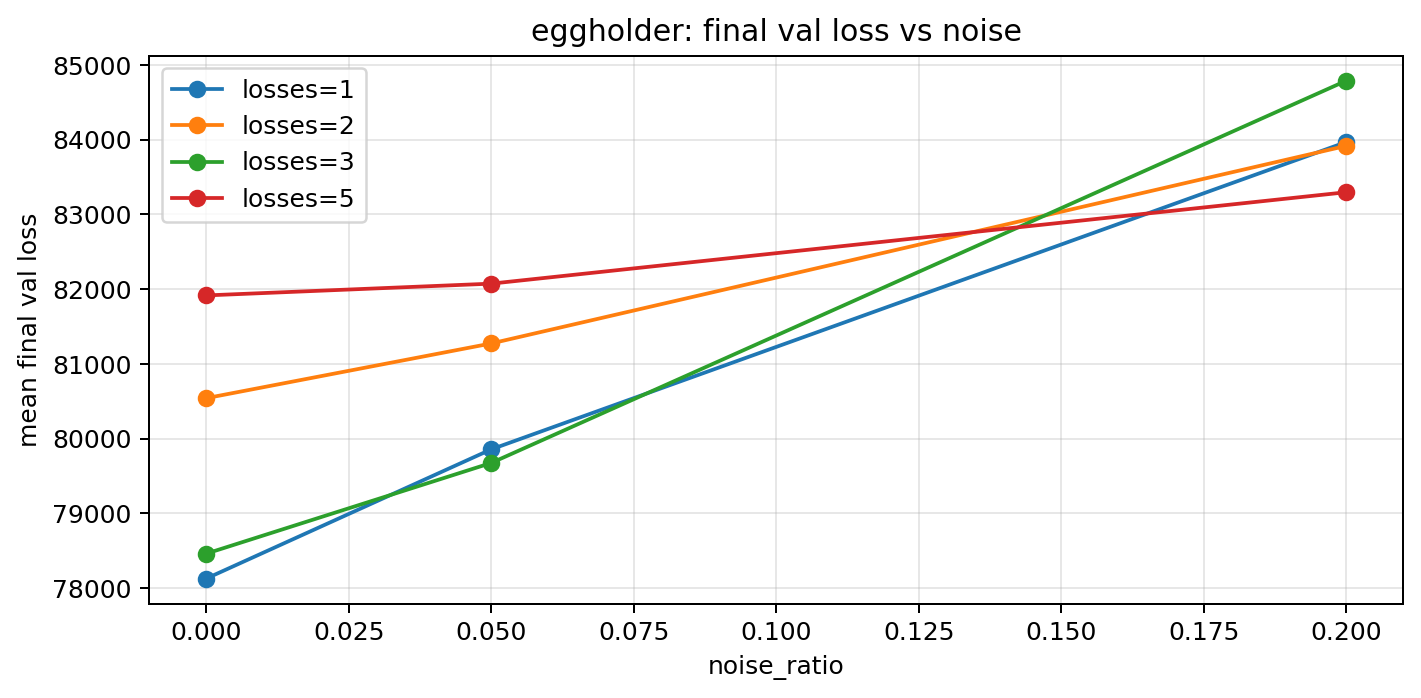
\includegraphics[width=0.92\textwidth]{figures/meta_weighting_eggholder_u1_final_val_loss_vs_noise.png}
    \caption{Mean final validation loss versus noise ratio. Performance generally degrades as noise increases, although the sensitivity depends on the number of losses.}
    \label{fig:meta-eggholder-u1-vs-noise}
\end{figure}

\begin{figure}[h]
    \centering
    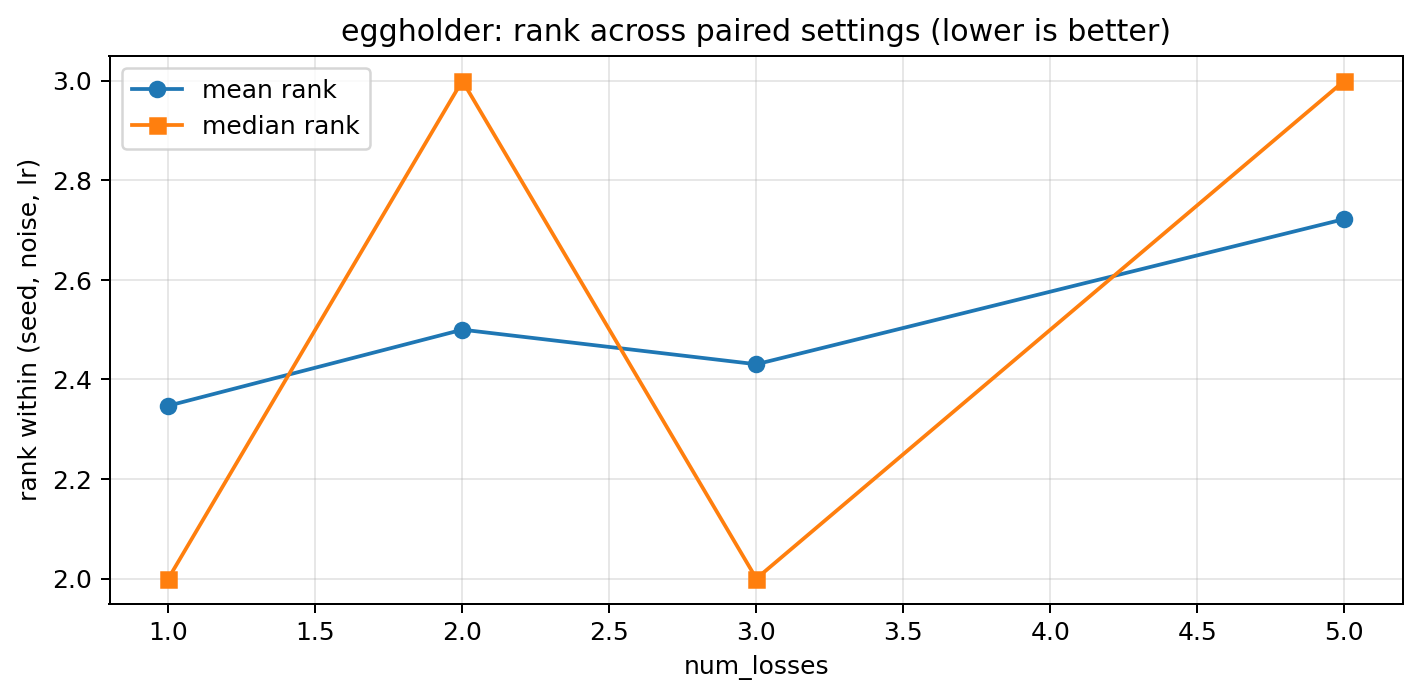
\includegraphics[width=0.72\textwidth]{figures/meta_weighting_eggholder_u1_rank_vs_num_losses.png}
    \caption{Average rank within matched settings (same seed, noise, and learning rates). Lower is better. The single-loss baseline ranks best on average, with the 3-loss setting closest behind.}
    \label{fig:meta-eggholder-u1-rank}
\end{figure}

\begin{figure}[h]
    \centering
    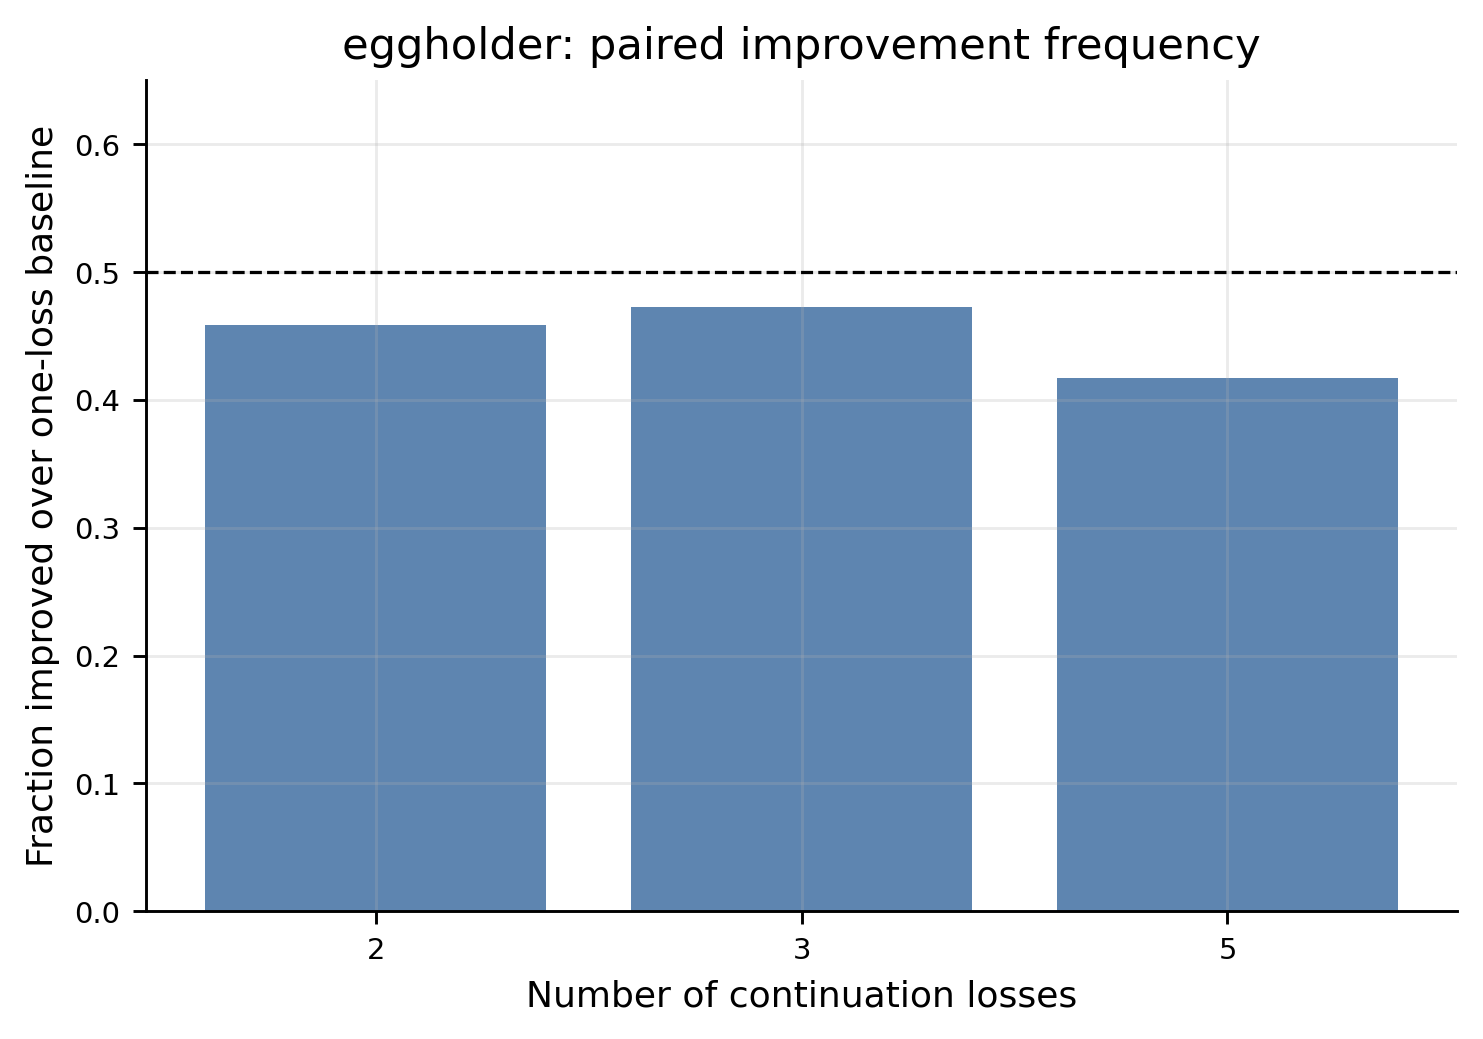
\includegraphics[width=0.72\textwidth]{figures/meta_weighting_eggholder_u1_win_rate_vs_baseline.png}
    \caption{Fraction of adaptive-weighting runs that improve over the baseline \texttt{num\_losses=1}. A value above 0.5 would indicate an advantage over the baseline. None of the adaptive settings exceed this threshold.}
    \label{fig:meta-eggholder-u1-fraction-improved}
\end{figure}

\begin{figure}[h]
    \centering
    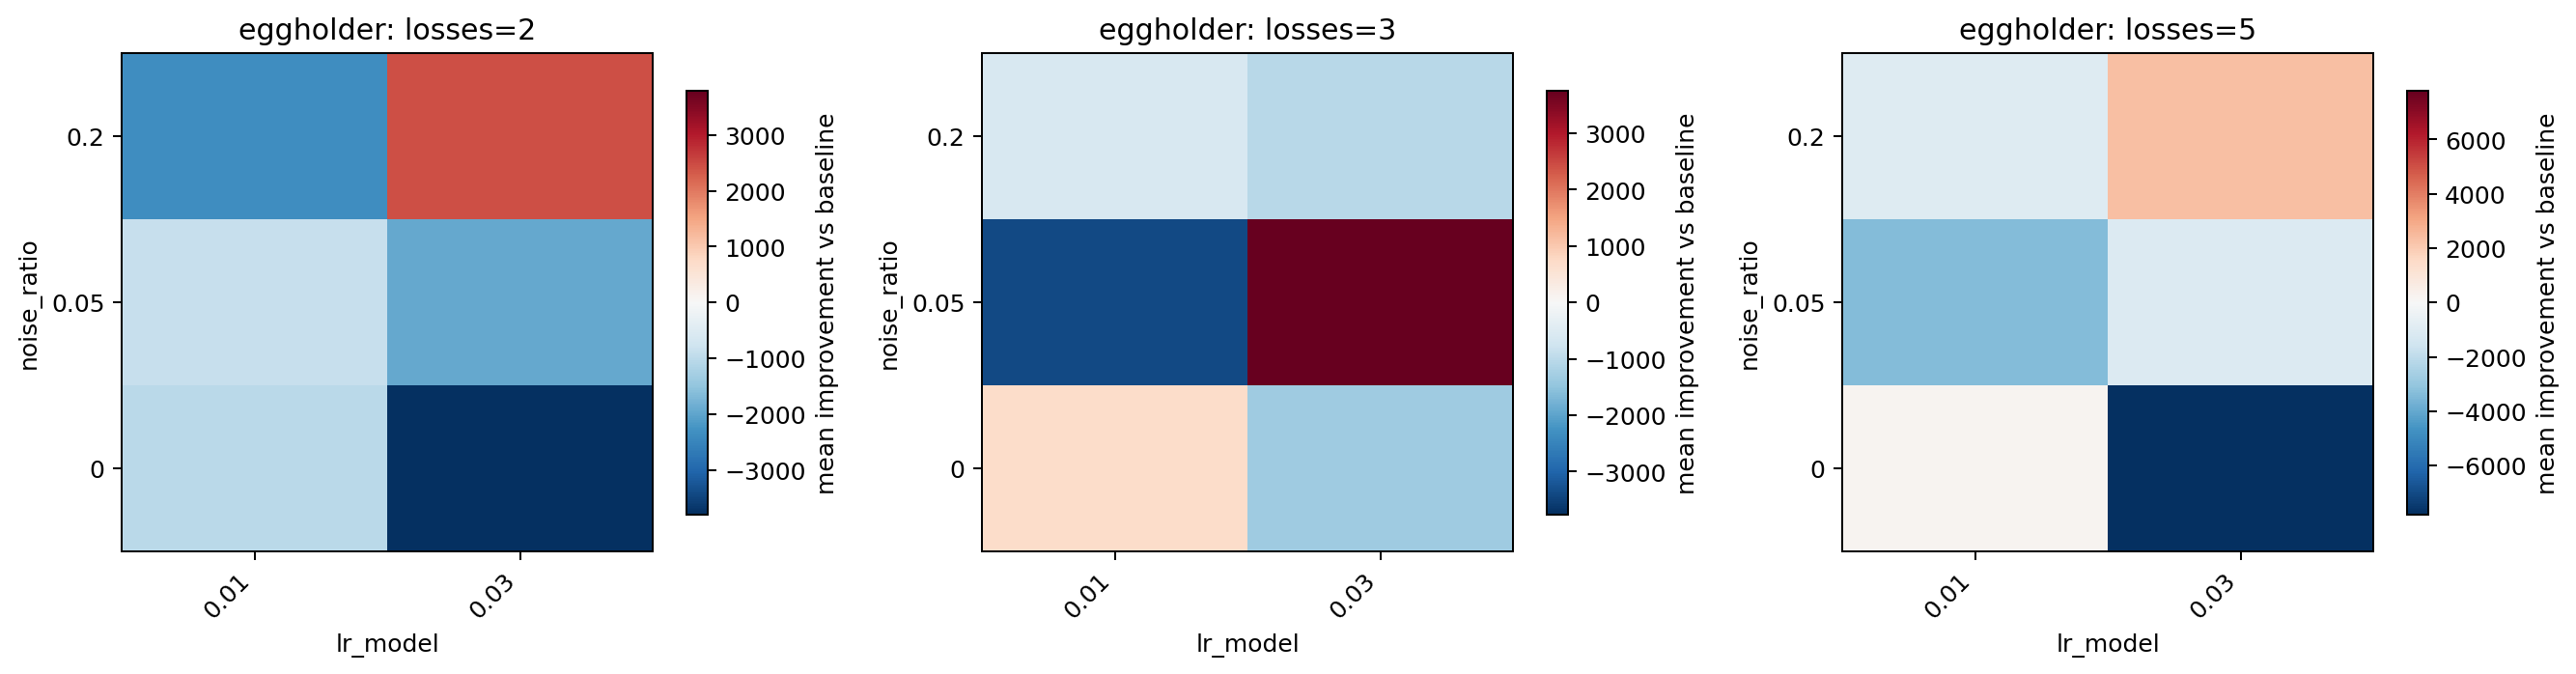
\includegraphics[width=0.88\textwidth]{figures/meta_weighting_eggholder_u1_improvement_heatmap.png}
    \caption{Mean improvement over the baseline across noise ratios and learning rates. Blue regions indicate settings where adaptive weighting improves over the baseline, while red regions indicate degradation. The pattern is mixed rather than uniformly favorable.}
    \label{fig:meta-eggholder-u1-heatmap}
\end{figure}

\section{Representative run dynamics}

To complement aggregate statistics, the next two figures show the best single
run found in the benchmark.

\begin{figure}[h]
    \centering
    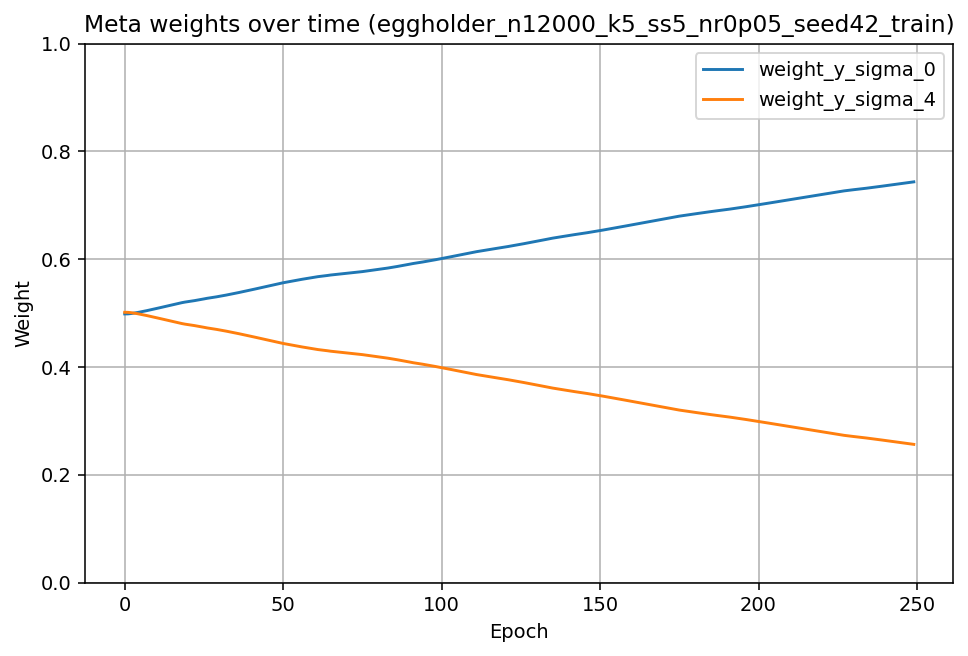
\includegraphics[width=0.82\textwidth]{figures/meta_weighting_eggholder_u1_best_weight_trajectory.png}
    \caption{Weight trajectory for the best single run (seed 42, noise 0.05, \texttt{num\_losses=2}, $\eta_{\mathrm{model}}=0.03$, $\eta_{\mathrm{meta}}=0.003$). This plot is useful for checking whether the meta-optimizer maintains a non-trivial balance between the selected losses over training.}
    \label{fig:meta-eggholder-u1-best-weights}
\end{figure}

\begin{figure}[h]
    \centering
    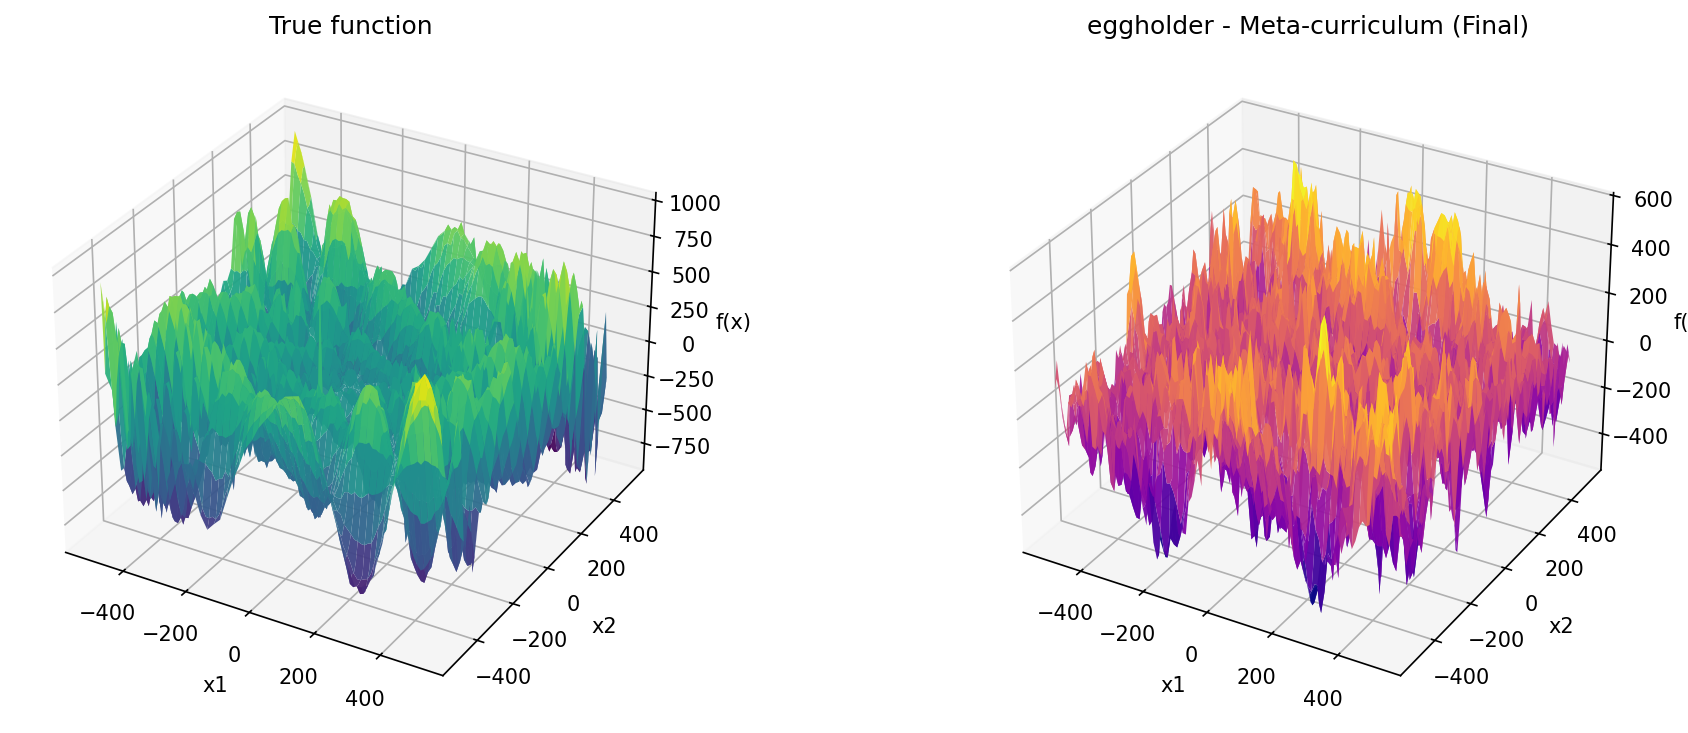
\includegraphics[width=0.78\textwidth]{figures/meta_weighting_eggholder_u1_best_final_surface.png}
    \caption{Final learned surface for the best single run according to hard validation loss.}
    \label{fig:meta-eggholder-u1-best-surface}
\end{figure}

\section{Interpretation}

\paragraph{1) Stability result.}
Restricting the meta-objective to a one-step lookahead was sufficient to make
all 288 runs complete successfully. This is an important methodological result,
because the longer unroll variants were substantially less stable in earlier
attempts.

\paragraph{2) Baseline strength.}
The single hard-target baseline remains difficult to outperform. Although adaptive
weighting sometimes finds very strong runs, its average behavior is not clearly
superior in this benchmark.

\paragraph{3) Best adaptive region.}
If adaptive weighting is pursued further for \texttt{eggholder}, the most
promising region from this benchmark appears to be:
\begin{itemize}
    \item higher model learning rate: \texttt{0.03},
    \item moderate-to-high meta learning rate: \texttt{0.001} to \texttt{0.003},
    \item a small number of losses: especially \texttt{2} or \texttt{3}.
\end{itemize}

\paragraph{4) Cost-benefit tradeoff.}
Using more weighted losses does not automatically improve the final hard-target
objective. In fact, the 5-loss setting is the most expensive conceptually and
performs worst on average in this experiment.

\section{Practical conclusion}

For the current thesis codebase and the \texttt{eggholder} benchmark,
meta-weighting with \texttt{meta\_unroll\_steps}=1 is operationally feasible and
produces interpretable weight trajectories, but it does not yet justify
replacing the direct hard-target baseline as the default method.

The most defensible conclusion at this stage is therefore:
\begin{itemize}
    \item keep \texttt{num\_losses=1} as the primary baseline,
    \item treat adaptive weighting as an exploratory extension,
    \item focus follow-up work on the narrower region where adaptive weighting
          showed occasional gains (2--3 losses, higher model LR, moderate/high
          meta LR).
\end{itemize}

% Appendix generated from W&B-exported CIFAR-100 model-size curriculum runs.
\chapter{CIFAR-100 Model-Size Study for Coarse-to-Fine Curriculum Learning}
\label{app:cifar100-model-size-curriculum}

\section{Purpose}

This appendix summarizes the first CIFAR-100 model-size study for the
coarse-to-fine curriculum learning reproduction. The main question was whether
the curriculum remains useful as the model becomes larger or architecturally
stronger. A secondary goal was to check whether macro-F1, top-5 accuracy,
hierarchy-aware scores, and calibration tell the same story as top-1 accuracy.

The runs are best read as a screening study. They show where the curriculum is
promising and where it is not, but they do not by themselves settle questions of
statistical stability or optimization-landscape smoothness. The roughness and
sharpness diagnostics were not active in this batch, so the direct Hessian and
sharpness question is taken up in Appendix~\ref{app:roughness-followup-curriculum}.

\section{Experimental protocol}

The analysis uses 80 completed runs from the CIFAR-100 model-size sweep. The
runs were grouped by model, architecture family, and curriculum length before
aggregation.

The common training protocol was:

\begin{itemize}
    \item dataset: CIFAR-100,
    \item seed: 42,
    \item optimizer: Adam,
    \item learning rate: 0.001,
    \item scheduler: none,
    \item batch size: 128,
    \item training budget: 100 epochs,
    \item curriculum lengths: 5, 10, 20, 30, and 40 epochs,
    \item checkpoints disabled.
\end{itemize}

Each model configuration was run as a Figure-11-style sweep consisting of one
baseline and five curriculum runs. The omitted length 50 was intentionally not
used in this study, because earlier runs suggested that very long hard curricula
mostly delay fine-label specialization.

The analyzed model ladder consisted of:

\begin{itemize}
    \item width-scaled CNNs: \texttt{cnn\_w0.5}, \texttt{cnn\_w1},
          \texttt{cnn\_w2}, and \texttt{cnn\_w4},
    \item CIFAR-style ResNets with depths 8, 20, 32, and 56,
    \item ImageNet-style ResNet adapted to CIFAR: \texttt{resnet18}.
\end{itemize}

The \texttt{cnn\_w0.5} job appears to have been restarted several times on
Runpod before the auto-stop logic was corrected. These repeated runs have the
same seed and configuration, so they are not independent random seeds. For the
summary tables below, repeated runs with the same model and curriculum length
were averaged. All other model configurations have one run per curriculum
length.

Because this sweep is mostly single-seed, it should be interpreted as an
exploratory map of the effect rather than a final significance test. The
multi-seed follow-up in Appendix~\ref{app:roughness-followup-curriculum}
rechecks the most important CIFAR-100 cases.

\section{Primary results: curriculum benefit versus model size}

Table~\ref{tab:cifar100-model-size-best} reports, for each model, the best
curriculum length according to best test accuracy, its gain over the baseline,
and the corresponding AUC gain. Accuracy gains are shown in percentage points.

\begin{table}[h]
\centering
\small
\begin{tabular}{lrrrrrr}
\hline
Model & Params & Base & Best CL & CL acc. & Gain & AUC gain \\
\hline
\texttt{cnn\_w0.5} & 65,636 & 0.3478 & 20 & 0.3796 & +3.18 & -4.08 \\
\texttt{cifar\_resnet8} & 83,892 & 0.5268 & 20 & 0.5449 & +1.81 & -5.94 \\
\texttt{cnn\_w1} & 158,820 & 0.3849 & 10 & 0.4211 & +3.62 & -2.29 \\
\texttt{cifar\_resnet20} & 278,324 & 0.6028 & 10 & 0.6047 & +0.19 & -4.22 \\
\texttt{cnn\_w2} & 428,132 & 0.4256 & 5 & 0.4472 & +2.16 & -0.81 \\
\texttt{cifar\_resnet32} & 472,756 & 0.6172 & 10 & 0.6207 & +0.35 & -2.79 \\
\texttt{cifar\_resnet56} & 861,620 & 0.6314 & 20 & 0.6233 & -0.81 & -7.04 \\
\texttt{cnn\_w4} & 1,298,532 & 0.4463 & 5 & 0.4447 & -0.16 & -3.35 \\
\texttt{resnet18} & 11,220,132 & 0.6876 & 20 & 0.6937 & +0.61 & -6.44 \\
\hline
\end{tabular}
\caption{Best curriculum run per model on CIFAR-100. Gain and AUC gain are
reported in percentage points relative to the matching baseline.}
\label{tab:cifar100-model-size-best}
\end{table}

Here, ``best test accuracy'' means the best point reached along the test
trajectory. This is useful for understanding the learning dynamics, but it is
not a deployment-style model-selection rule. In a stricter protocol, the epoch
would be selected on validation data and the test set would be used only once at
the selected epoch. The AUC column is the normalized area under the per-epoch
test-accuracy curve; a negative AUC gain means that the curriculum spent much of
training below the baseline trajectory even if it later reached a better peak.

The strongest curriculum benefits occur in the smaller CNNs. The largest gain is
observed for \texttt{cnn\_w1} (+3.62 percentage points), followed by
\texttt{cnn\_w0.5} (+3.18 points) and \texttt{cnn\_w2} (+2.16 points). In
contrast, the largest CNN, \texttt{cnn\_w4}, no longer benefits. The CIFAR-style
ResNets also show a capacity-dependent pattern: \texttt{cifar\_resnet8} gains
+1.81 points, while \texttt{cifar\_resnet20} and \texttt{cifar\_resnet32} are
almost unchanged, and \texttt{cifar\_resnet56} is worse than baseline.

The ImageNet-style \texttt{resnet18} achieves the highest absolute accuracy and
shows a small positive best-accuracy gain (+0.61 points), but this gain is much
smaller than the gains seen in the smaller CNNs. Moreover, its AUC gain is
negative, which means that the curriculum run was not faster or better over the
whole training trajectory.

\begin{figure}[h]
    \centering
    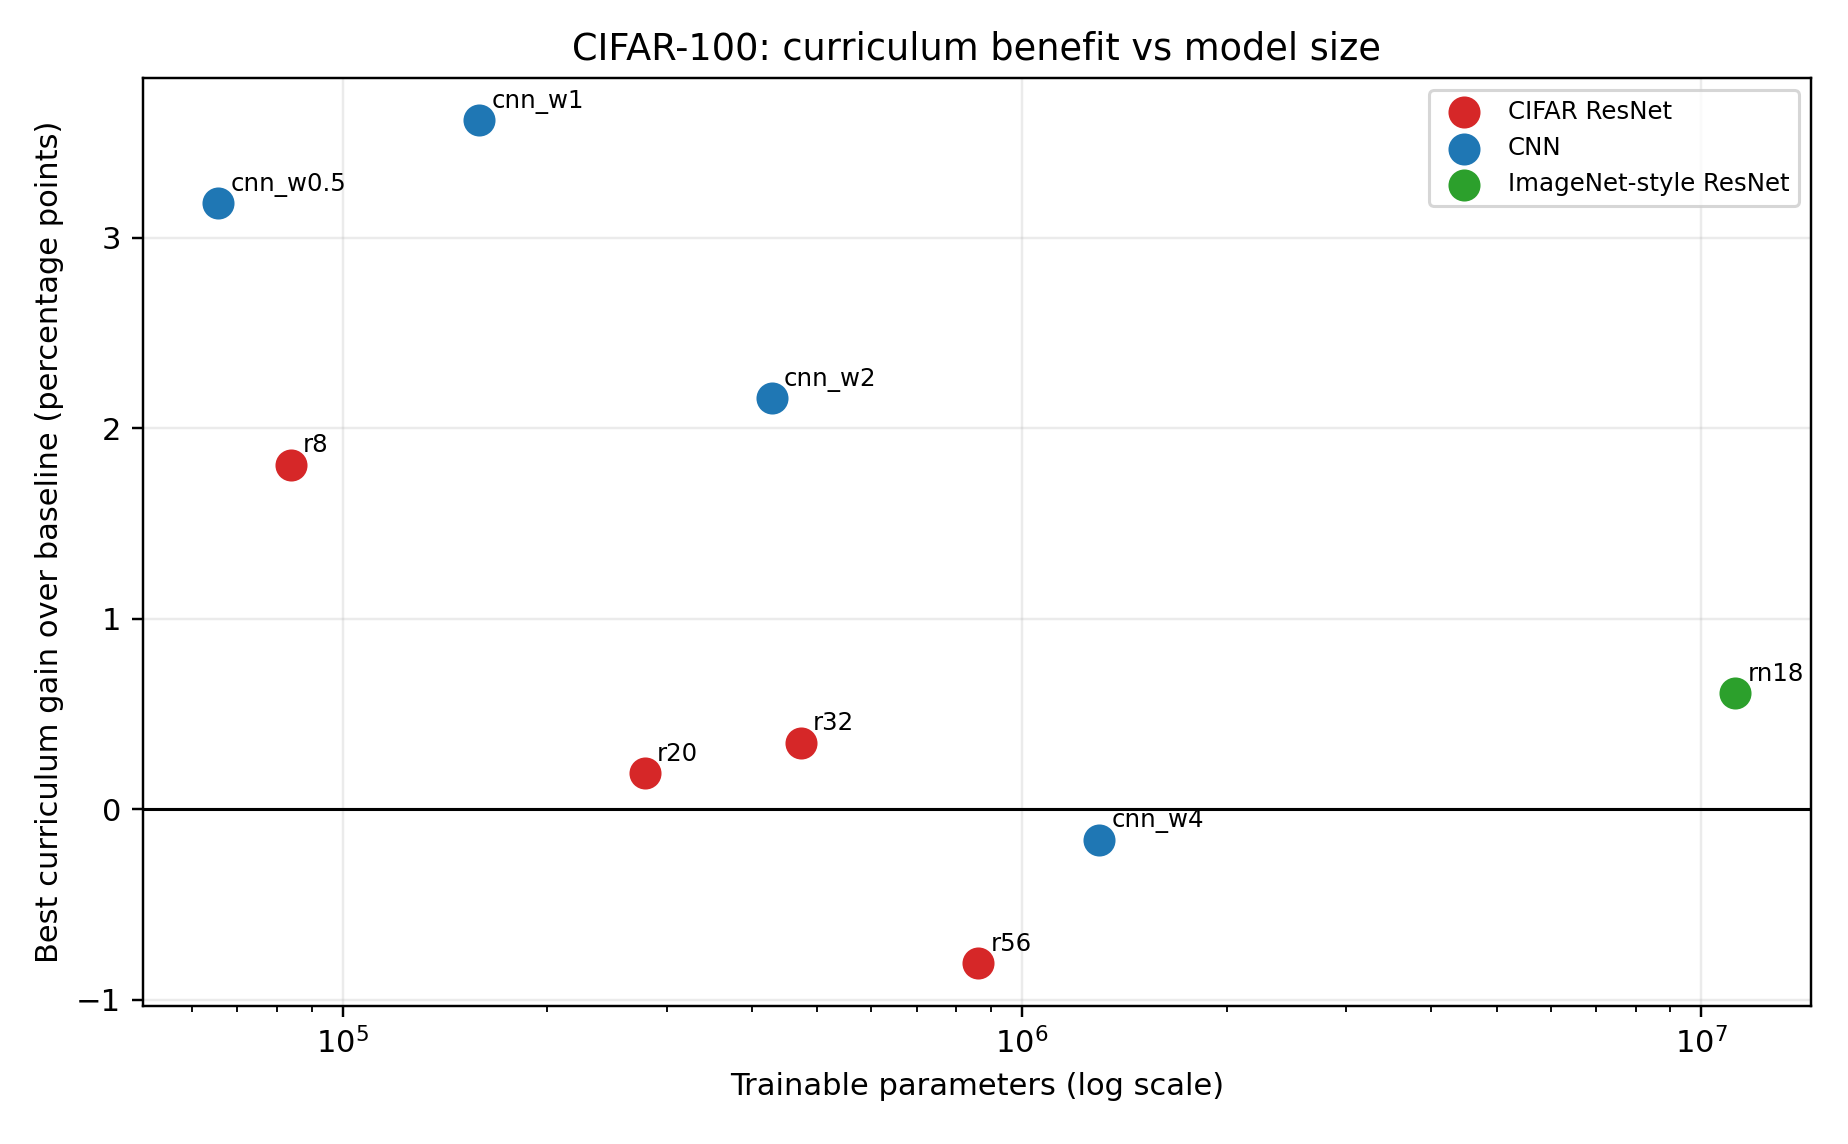
\includegraphics[width=0.90\textwidth]{figures/cifar100_model_size_gain_vs_params.png}
    \caption{Best curriculum gain over baseline as a function of trainable
    parameter count. The strongest gains occur for smaller CNNs, while larger
    CNNs and deeper CIFAR ResNets show little or negative benefit.}
    \label{fig:cifar100-model-size-gain-vs-params}
\end{figure}

\section{Curriculum length sensitivity}

Table~\ref{tab:cifar100-model-size-lengths} shows the best test accuracy for all
curriculum lengths. The baseline is represented as length 0.

\begin{table}[h]
\centering
\small
\begin{tabular}{lrrrrrr}
\hline
Model & Base & CL5 & CL10 & CL20 & CL30 & CL40 \\
\hline
\texttt{cnn\_w0.5} & 0.3478 & 0.3757 & 0.3783 & 0.3796 & 0.3729 & 0.3634 \\
\texttt{cifar\_resnet8} & 0.5268 & 0.5243 & 0.5321 & 0.5449 & 0.5228 & 0.5318 \\
\texttt{cnn\_w1} & 0.3849 & 0.4188 & 0.4211 & 0.4070 & 0.3820 & 0.3708 \\
\texttt{cifar\_resnet20} & 0.6028 & 0.5857 & 0.6047 & 0.5966 & 0.5869 & 0.5826 \\
\texttt{cnn\_w2} & 0.4256 & 0.4472 & 0.4250 & 0.4030 & 0.3824 & 0.3828 \\
\texttt{cifar\_resnet32} & 0.6172 & 0.6177 & 0.6207 & 0.6143 & 0.6143 & 0.6091 \\
\texttt{cifar\_resnet56} & 0.6314 & 0.6195 & 0.6224 & 0.6233 & 0.6218 & 0.6118 \\
\texttt{cnn\_w4} & 0.4463 & 0.4447 & 0.4319 & 0.4041 & 0.3950 & 0.3825 \\
\texttt{resnet18} & 0.6876 & 0.6884 & 0.6915 & 0.6937 & 0.6849 & 0.6871 \\
\hline
\end{tabular}
\caption{Best test accuracy by curriculum length on CIFAR-100.}
\label{tab:cifar100-model-size-lengths}
\end{table}

A clear qualitative pattern appears within the CNN family. As CNN width
increases, the best curriculum becomes shorter:

\begin{itemize}
    \item \texttt{cnn\_w0.5}: best at 20 curriculum epochs,
    \item \texttt{cnn\_w1}: best at 10 curriculum epochs,
    \item \texttt{cnn\_w2}: best at 5 curriculum epochs,
    \item \texttt{cnn\_w4}: no useful curriculum length.
\end{itemize}

This is consistent with the interpretation that smaller models need more help
from coarse supervision, while stronger CNNs need either only a short curriculum
or no hard curriculum at all.

\begin{figure}[h]
    \centering
    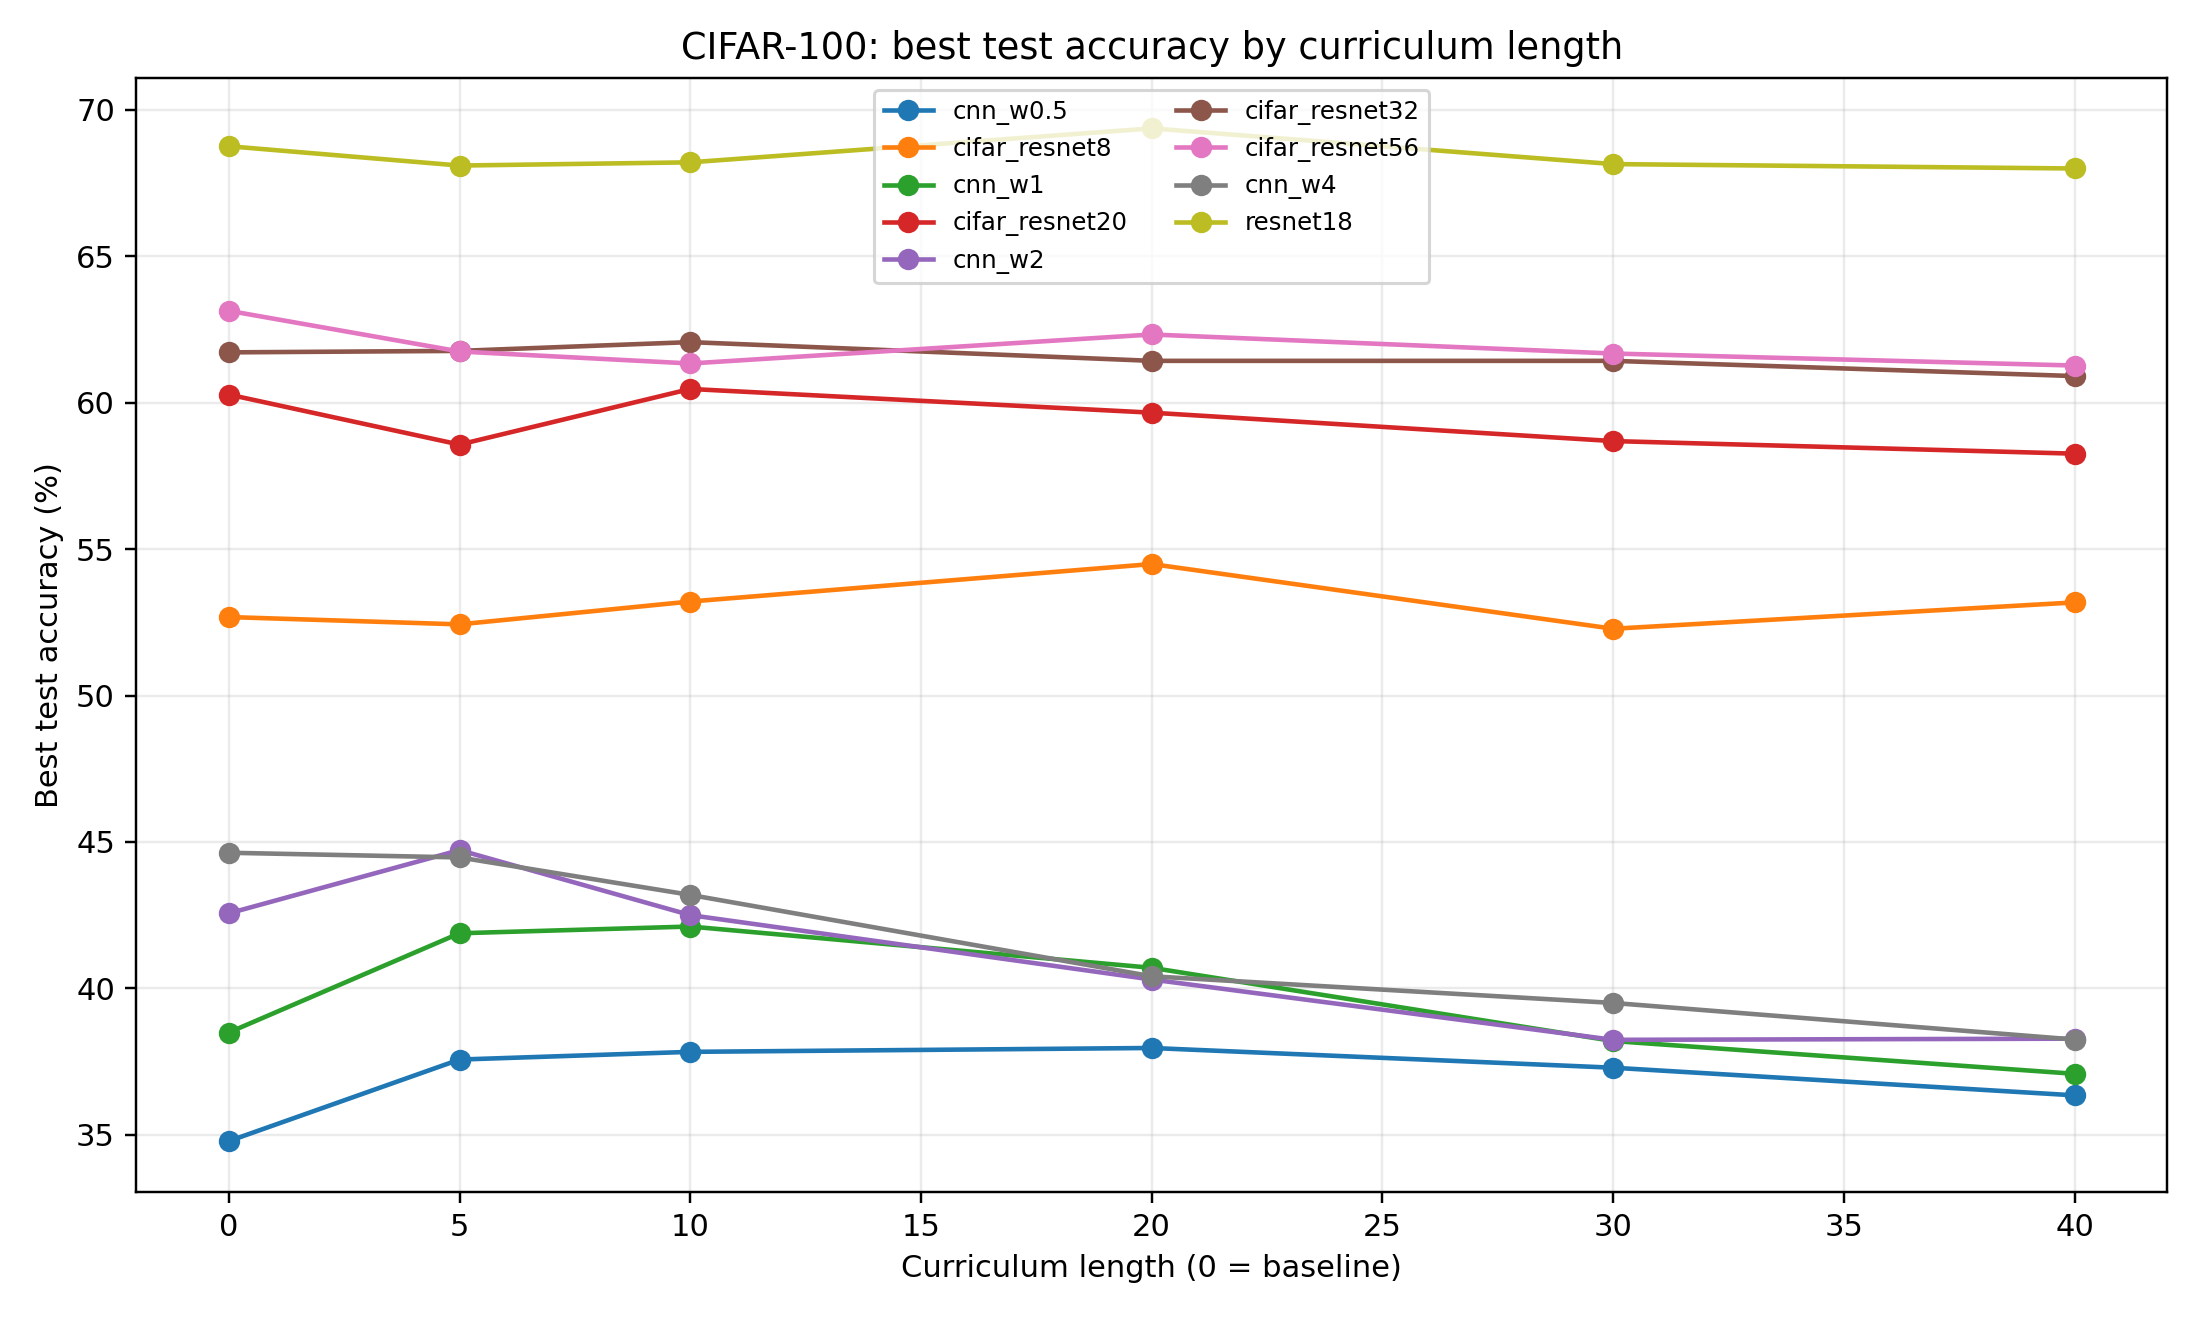
\includegraphics[width=0.95\textwidth]{figures/cifar100_model_size_curriculum_lengths.png}
    \caption{Best test accuracy by curriculum length. Length 0 denotes the
    baseline. Long curricula hurt most larger models, while small CNNs benefit
    from moderate curriculum lengths.}
    \label{fig:cifar100-model-size-curriculum-lengths}
\end{figure}

\section{Speed and AUC}

The curriculum runs generally do not improve the full test-accuracy trajectory.
Figure~\ref{fig:cifar100-model-size-auc-gain} shows the AUC gain for the best
curriculum run of each model. All values are negative.

\begin{figure}[h]
    \centering
    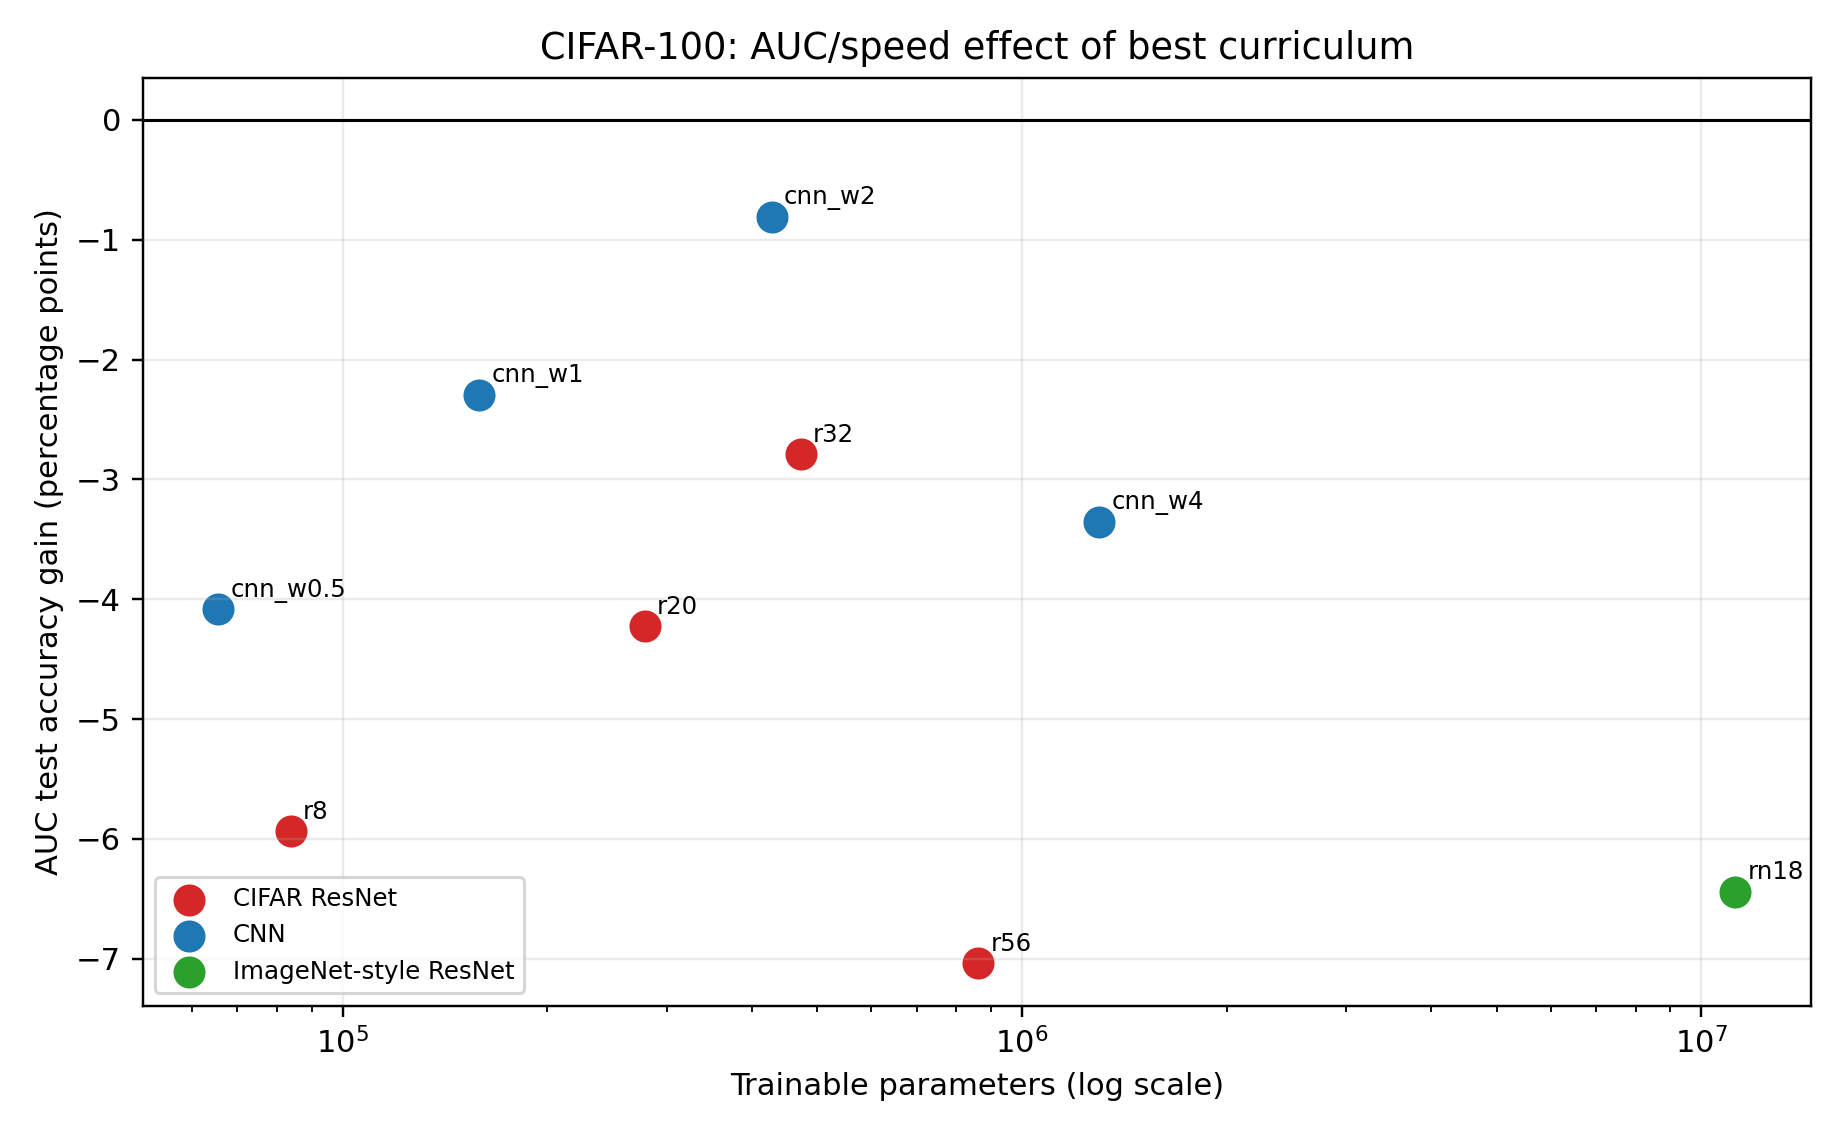
\includegraphics[width=0.90\textwidth]{figures/cifar100_model_size_auc_gain.png}
    \caption{AUC test-accuracy gain for the best curriculum run per model. The
    best curriculum can improve peak accuracy while still lowering AUC, because
    early coarse stages delay fine-label accuracy.}
    \label{fig:cifar100-model-size-auc-gain}
\end{figure}

This changes the interpretation of the curriculum effect. These runs do not show
that hard coarse-to-fine curriculum learning makes training uniformly faster.
Instead, the evidence suggests that curriculum can improve the best solution
encountered by smaller models, while sacrificing some early fine-label
performance.

\section{Metrics beyond accuracy}

The alternative metrics generally agree with the accuracy results. For the
models that benefit most in top-1 accuracy, curriculum also improves macro-F1,
top-5 accuracy, and hierarchy-aware scores. For models with weak or negative
accuracy gains, the alternative metrics are also weak or negative. The official
hierarchy-aware score gives partial credit when the prediction falls in the same
CIFAR-100 superclass as the target, so it measures whether mistakes remain close
in the human-defined class hierarchy.

\begin{table}[h]
\centering
\small
\begin{tabular}{lrrrrr}
\hline
Model & Acc. gain & F1 gain & Top-5 gain & Official hier. gain & ECE delta \\
\hline
\texttt{cnn\_w0.5} & +3.18 & +1.33 & +1.37 & +1.63 & +2.96 \\
\texttt{cifar\_resnet8} & +1.81 & +2.69 & +1.37 & +2.71 & -1.41 \\
\texttt{cnn\_w1} & +3.62 & +1.37 & +2.89 & +1.91 & +1.22 \\
\texttt{cifar\_resnet20} & +0.19 & -0.18 & +0.16 & -0.08 & -2.61 \\
\texttt{cnn\_w2} & +2.16 & +0.51 & +0.80 & +0.58 & +0.60 \\
\texttt{cifar\_resnet32} & +0.35 & +0.28 & +0.38 & +0.47 & -1.04 \\
\texttt{cifar\_resnet56} & -0.81 & -0.22 & -0.79 & -0.27 & -1.03 \\
\texttt{cnn\_w4} & -0.16 & -0.77 & -1.15 & -1.15 & +2.01 \\
\texttt{resnet18} & +0.61 & +0.37 & +0.44 & +0.44 & -0.48 \\
\hline
\end{tabular}
\caption{Alternative metric changes for the best curriculum run of each model.
All values except ECE are percentage-point gains relative to baseline. Negative
ECE delta indicates improved calibration.}
\label{tab:cifar100-model-size-alt-metrics}
\end{table}

The hierarchy-aware metrics are especially relevant because coarse-to-fine
curriculum learning is explicitly hierarchical. Figure~\ref{fig:cifar100-model-size-hier-gain}
compares exact top-1 gain against the official CIFAR-100 hierarchy-score gain.
Most models lie in the expected quadrants: when top-1 accuracy improves, the
hierarchical score also improves.

\begin{figure}[h]
    \centering
    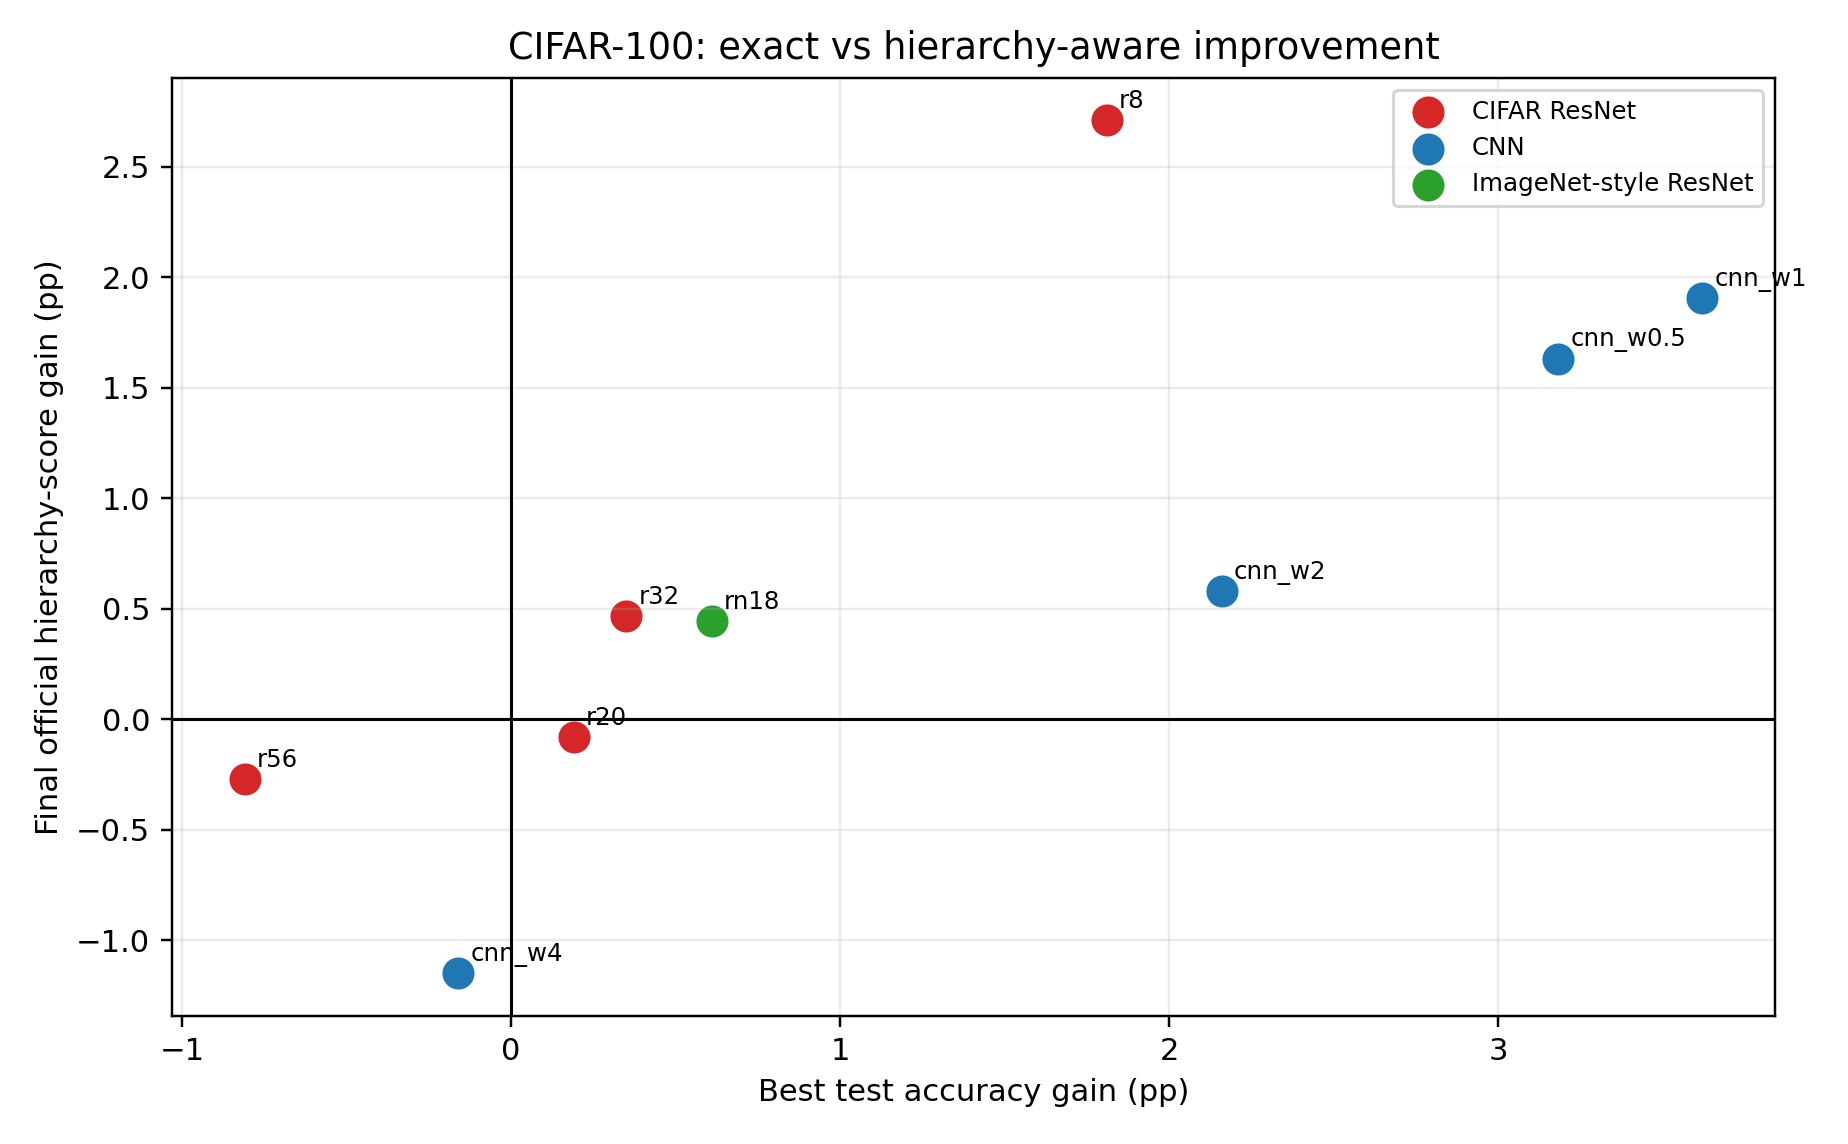
\includegraphics[width=0.90\textwidth]{figures/cifar100_model_size_hier_gain.png}
    \caption{Relationship between exact top-1 improvement and official
    hierarchy-score improvement. For the smaller models, curriculum improves both
    exact and hierarchy-aware behavior.}
    \label{fig:cifar100-model-size-hier-gain}
\end{figure}

Calibration behaves differently across architecture families. CNN curricula tend
to worsen ECE even when accuracy improves, suggesting more overconfident
predictions. CIFAR ResNets and ResNet-18 often show slightly improved ECE under
their best curriculum runs.

\section{Sharpness and landscape smoothness}

No direct conclusion about sharpness or optimization-landscape smoothing can be
drawn from this batch, because the roughness diagnostics were not active. This
is a limitation of the data collected here, not evidence for or against the
method itself. In particular, the accuracy gains in this appendix should not be
read as proof that the curriculum finds flatter minima. Appendix~\ref{app:roughness-followup-curriculum}
adds a focused roughness follow-up and shows that the picture is mixed.

\section{Interpretation}

The current evidence supports a capacity-conditioned view of hard
coarse-to-fine curriculum learning:

\begin{quote}
On CIFAR-100, hard coarse-to-fine curriculum learning is most useful for
low-capacity CNNs. As model width, residual depth, or architecture strength
increases, the benefit shrinks or disappears. The curriculum can improve peak
accuracy and hierarchy-aware behavior, but it usually does not improve the full
training trajectory as measured by AUC.
\end{quote}

This statement is stronger than a simple CNN-versus-ResNet comparison, because
there is now within-family evidence. In the CNN family, increasing width changes
the optimal curriculum from moderate length to short length and finally to no
benefit. In the CIFAR ResNet family, the smallest model benefits, while deeper
models show near-zero or negative gain.

The result should still be interpreted with care. The main sweep uses one random
seed, and architecture and capacity are not fully separable when comparing CNNs,
CIFAR ResNets, and ImageNet-style ResNet-18. The most defensible claim is
therefore that curriculum usefulness depends on both capacity and architecture,
with the strongest evidence for a within-family capacity effect in the CNN
models.

\section{Connection to the follow-up study}
\label{sec:cifar100-model-size-next-steps}

Appendix~\ref{app:roughness-followup-curriculum} follows this screening sweep in
three ways. First, it repeats the most important CIFAR-100 cases across three
seeds, so the single-seed pattern from this appendix can be checked for
stability. Second, it adds roughness and sharpness diagnostics for a smaller set
of representative models. Third, it tests whether the same curriculum idea
transfers to Fashion-MNIST, CIFAR-10, and Tiny ImageNet.

The main remaining gaps are now more targeted. The full model-size ladder was
not repeated across many seeds, and the reported peak test accuracy should be
complemented by test accuracy at the best validation epoch. The random-hierarchy
control is now covered in Appendix~\ref{app:hierarchy-ablation-curriculum},
which shows that matched random coarsening explains only part of the gain in the
main CIFAR-100 weak-CNN setting. The next open hierarchy question is broader:
how classifier-weight hierarchies compare with semantic or dataset-defined
hierarchies across multiple architectures.

% Appendix generated from W&B roughness follow-up runs.
\chapter{Roughness Follow-up, Dataset Controls, and Learned Hierarchies}
\label{app:roughness-followup-curriculum}

\section{Purpose}

Appendix~\ref{app:cifar100-model-size-curriculum} identified a capacity-dependent
pattern on CIFAR-100: coarse-to-fine curriculum learning helped the smaller CNNs
and the smallest CIFAR-style ResNet, while the benefit shrank for larger models.
This appendix reports the follow-up experiments run after that result. The goals
were:

\begin{enumerate}
    \item to verify the CIFAR-100 pattern on multiple seeds for representative
          models, including the missing \texttt{cnn\_w0.5} case,
    \item to test whether roughness and sharpness probes explain the curriculum
          effect,
    \item to check whether the same behavior appears on smaller control datasets
          such as Fashion-MNIST and CIFAR-10,
    \item to run a minimal Tiny ImageNet pilot as a harder many-class stress
          test.
\end{enumerate}

The experiments were not intended as a full exhaustive sweep. They were designed
as targeted confirmation and diagnostic runs that could be completed while the
thesis was being written.

\section{Protocol and logged artifacts}

All runs were logged to W\&B in project
\texttt{curriculum-learning-ma/coarse-to-fine-curriculum}. The main analyzed
W\&B groups were:

\begin{itemize}
    \item \texttt{roughness-cifar100-appendix-f-cheap},
    \item \texttt{roughness-cifar100-w05-followup},
    \item \texttt{roughness-fashionmnist-control},
    \item \texttt{roughness-fashionmnist-w05-followup},
    \item \texttt{roughness-cifar10-control},
    \item \texttt{roughness-tinyimagenet-minimal}.
\end{itemize}

The CIFAR-100, Fashion-MNIST, and CIFAR-10 runs used seeds 42, 43, and 44. Tiny
ImageNet was run only as a one-seed pilot because of runtime cost. The main
training setup used Adam with learning rate 0.001 and no scheduler. CIFAR-100
was run for 200 epochs, while Fashion-MNIST and CIFAR-10 were run for 100
epochs. The Tiny ImageNet pilot was also run for 100 epochs.

Roughness probes logged critical sharpness, relative critical sharpness, Hessian
top-eigenvalue estimates, Hessian Frobenius estimates, Hessian trace estimates,
and gradient norm statistics. To reduce compute cost, these runs used one probe
batch and one Hessian iteration/sample. Therefore the roughness numbers should
be treated as coarse diagnostics rather than high-precision estimates. In
particular, gradient noise scale is not meaningful with only one probe batch.

For new runs, the learned hierarchy was also saved as both machine-readable JSON
and human-readable Markdown:

\begin{verbatim}
hierarchy.json
hierarchy.md
\end{verbatim}

The Markdown hierarchy is uploaded to W\&B as a run artifact and can be inspected
from the run page under \texttt{Artifacts}. This is especially useful for
Fashion-MNIST and CIFAR-10, where the number of classes is small enough that the
learned clusters can be read directly. These hierarchies are generated from the
baseline classifier-weight distances, not from official semantic metadata.

\section{Run completion summary}

The completed runs used in the updated analysis are summarized in
Table~\ref{tab:roughness-updated-run-summary}. One earlier Tiny ImageNet
\texttt{cnn\_w1} baseline was stopped before completion and excluded; a later
finished baseline was used instead.

\begin{table}[h]
\centering
\small
\begin{tabular}{llrl}
\hline
Dataset & W\&B group(s) & Finished runs & Design \\
\hline
CIFAR-100 & main + \texttt{w0.5} follow-up & 30 & 5 model pairs, 3 seeds \\
Fashion-MNIST & main + \texttt{w0.5} follow-up & 27 & 5 curriculum comparisons, 3 seeds \\
CIFAR-10 & control & 15 & 3 curriculum comparisons, 3 seeds \\
Tiny ImageNet & minimal pilot & 4 & 2 model pairs, 1 seed \\
\hline
\end{tabular}
\caption{Completed runs used in the updated roughness follow-up analysis.}
\label{tab:roughness-updated-run-summary}
\end{table}

\section{CIFAR-100 confirmation including \texttt{cnn\_w0.5}}

Table~\ref{tab:roughness-cifar100-updated} reports absolute best test accuracy
for the matching baseline and curriculum runs, together with the curriculum gain.
Values are averaged over seeds 42, 43, and 44. Gains are reported in percentage
points.

\begin{table}[h]
\centering
\small
\begin{tabular}{lrrrrr}
\hline
Model & Curriculum & Base best & Curr best & Gain & AUC gain \\
\hline
\texttt{cnn\_w0.5} & \texttt{curr20} & 0.3504 & 0.3758 & +2.54 & -1.72 \\
\texttt{cnn\_w1} & \texttt{curr10} & 0.3862 & 0.4060 & +1.98 & -0.23 \\
\texttt{cnn\_w2} & \texttt{curr5} & 0.4243 & 0.4415 & +1.72 & +0.15 \\
\texttt{cnn\_w4} & \texttt{curr5} & 0.4451 & 0.4485 & +0.34 & -1.03 \\
\texttt{cifar\_resnet8} & \texttt{curr20} & 0.5527 & 0.5660 & +1.33 & -1.96 \\
\hline
\end{tabular}
\caption{CIFAR-100 updated follow-up. Absolute best test accuracies are means
over seeds 42, 43, and 44.}
\label{tab:roughness-cifar100-updated}
\end{table}

The additional \texttt{cnn\_w0.5} runs strengthen the conclusion from
Appendix~\ref{app:cifar100-model-size-curriculum}. The weakest CNN obtains the
largest multi-seed gain in this follow-up (+2.54 percentage points), followed by
\texttt{cnn\_w1}, \texttt{cnn\_w2}, and \texttt{cifar\_resnet8}. The larger
\texttt{cnn\_w4} again has only a small best-accuracy improvement and worse AUC.
Thus, the capacity-conditioned pattern remains visible after adding the missing
smallest CNN.

\begin{figure}[h]
    \centering
    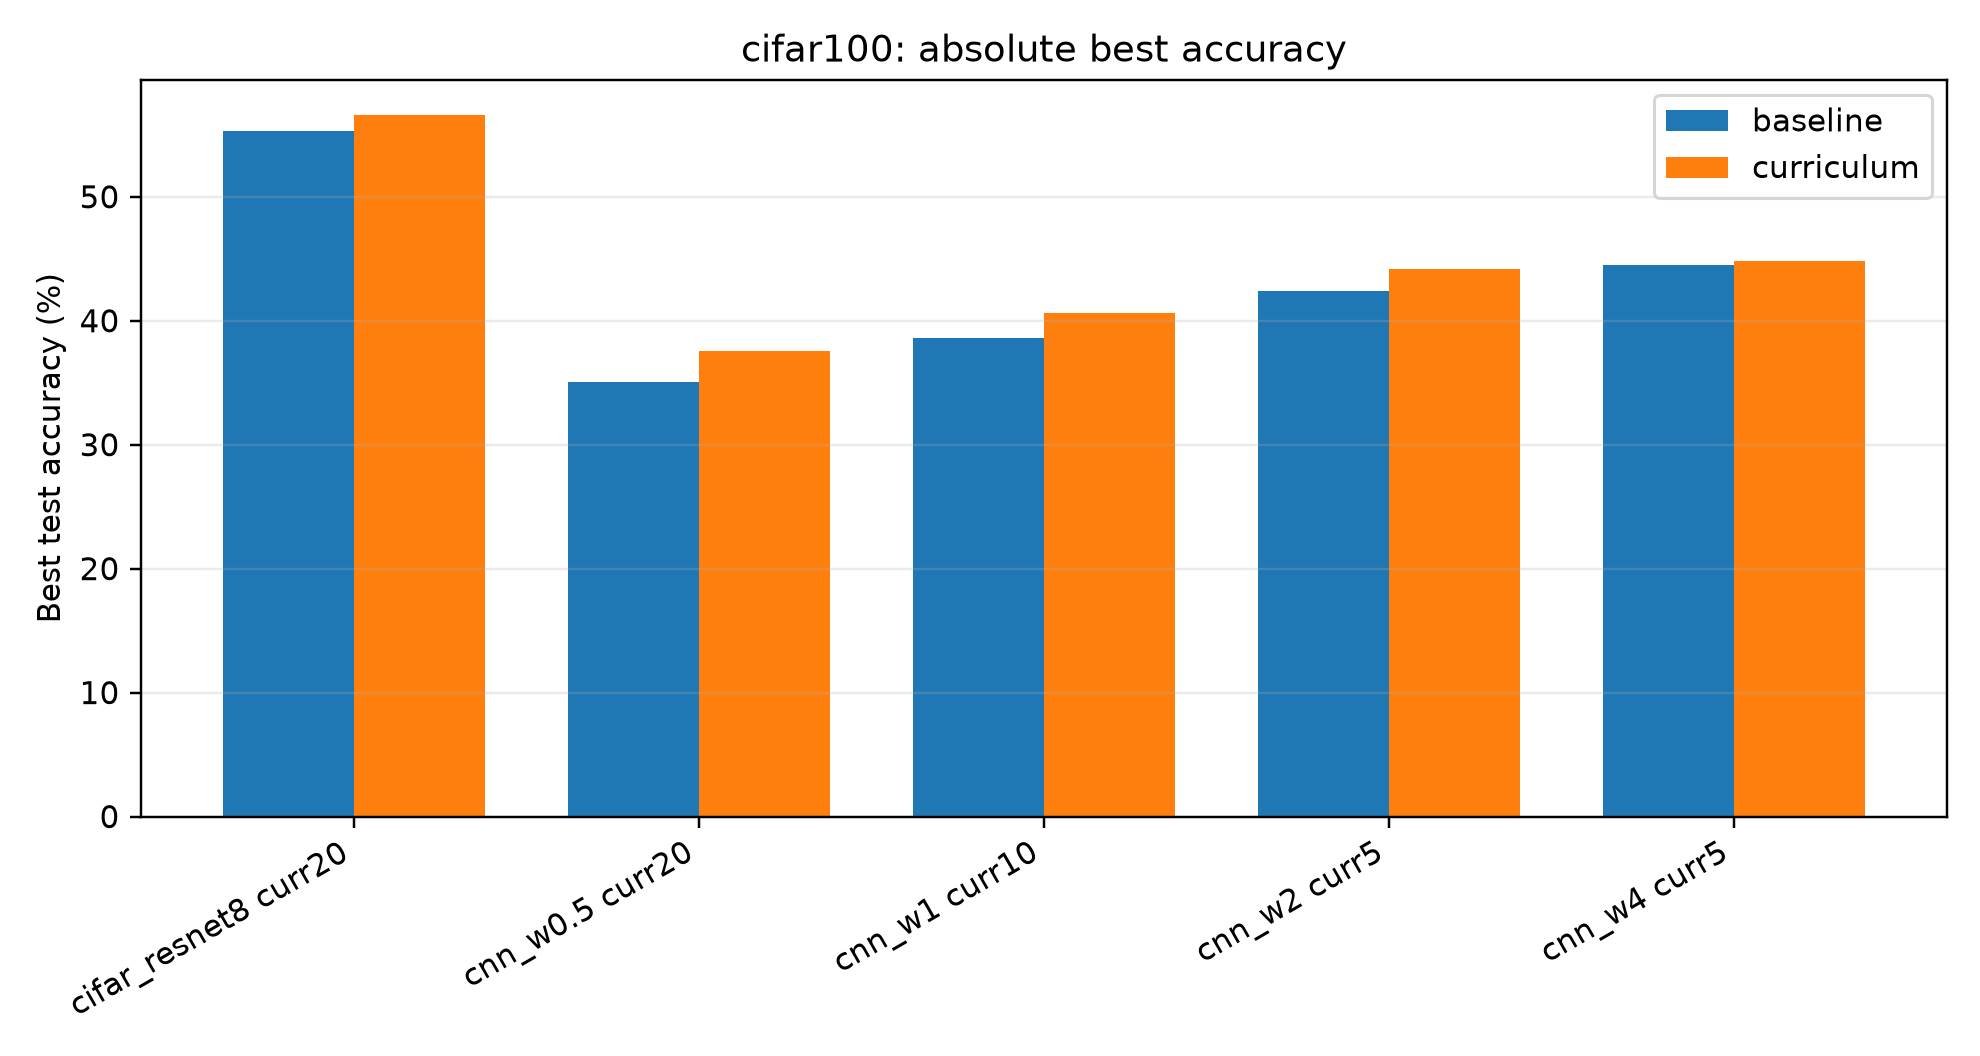
\includegraphics[width=0.82\textwidth]{figures/roughness_followup_updated_cifar100_absolute_best_acc.png}
    \caption{CIFAR-100 absolute best test accuracy for baseline and curriculum
    runs in the updated follow-up.}
    \label{fig:roughness-updated-cifar100-absolute}
\end{figure}

\begin{figure}[h]
    \centering
    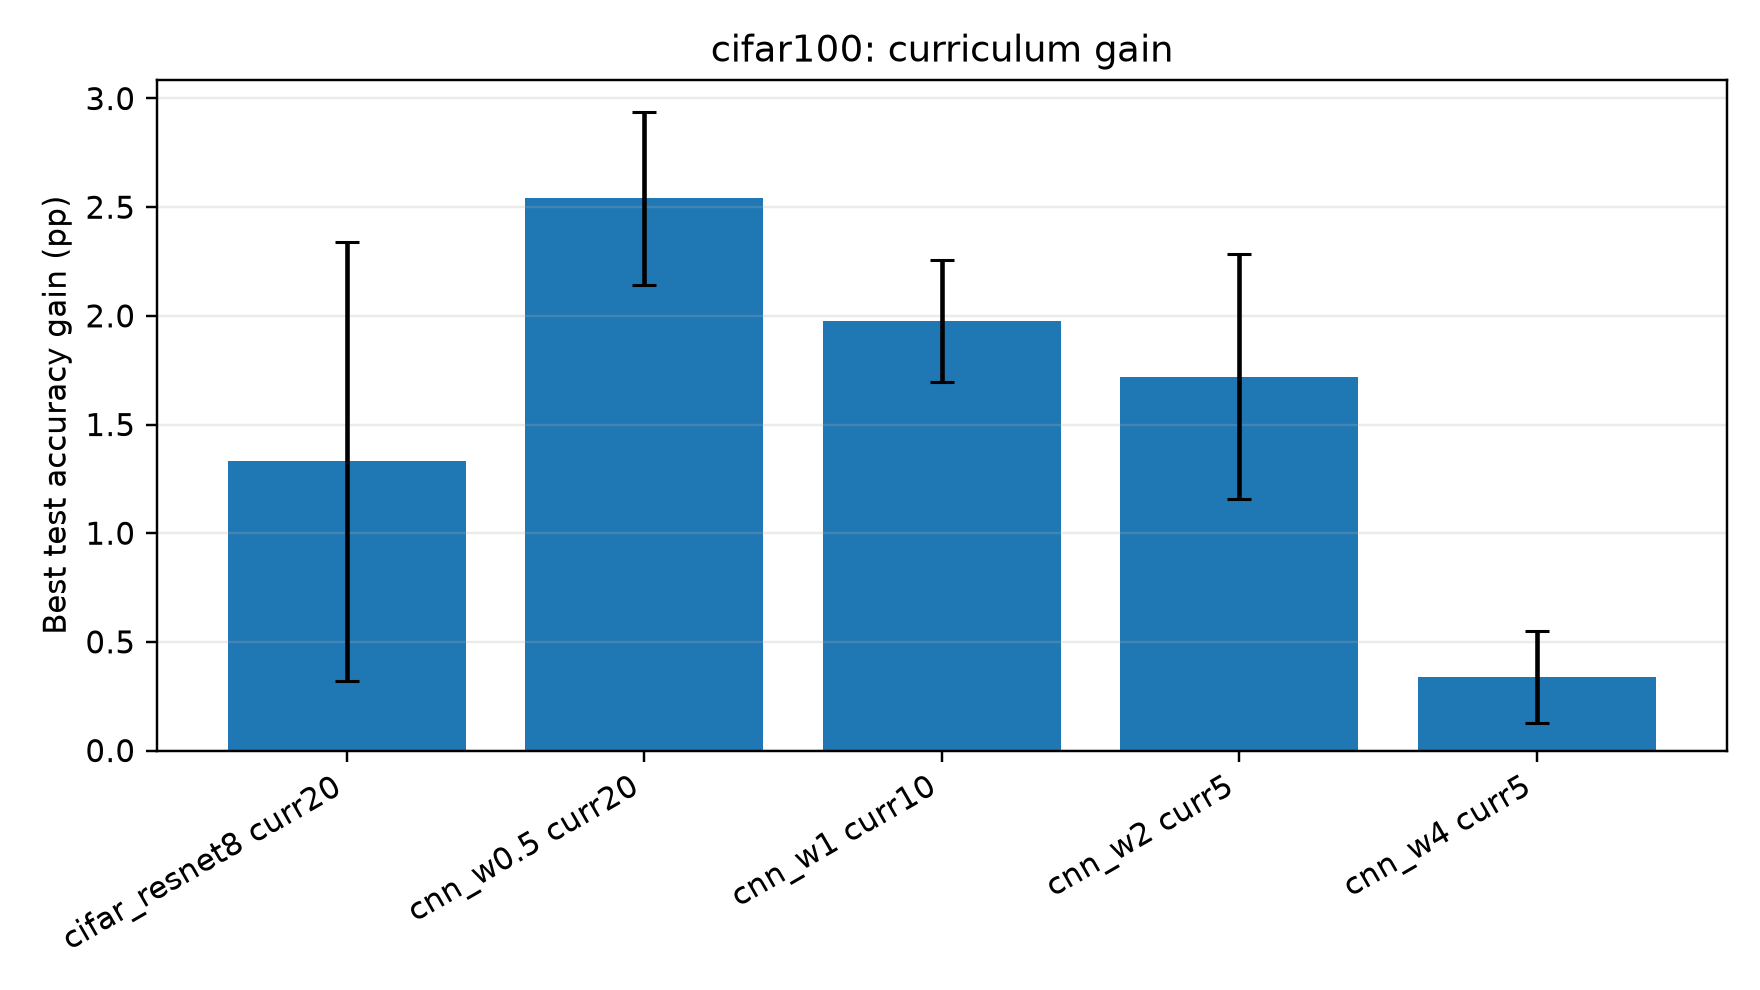
\includegraphics[width=0.82\textwidth]{figures/roughness_followup_updated_cifar100_best_acc_gains.png}
    \caption{CIFAR-100 curriculum gains in best test accuracy. Error bars show
    variation across seeds.}
    \label{fig:roughness-updated-cifar100-gains}
\end{figure}

A subtle point is that \texttt{cnn\_w0.5} improves strongly in best accuracy, but
its final epoch accuracy is almost unchanged. This means the weak CNN overfits or
drifts late in training. For this reason, best accuracy and AUC should both be
reported: curriculum can improve the best solution encountered while still
hurting the average trajectory.

\section{Fashion-MNIST control}

Fashion-MNIST was used as an easy 10-class control. The updated runs include the
original model set and an additional \texttt{cnn\_w0.5} follow-up with
\texttt{curr10} and \texttt{curr20}. Results are shown in
Table~\ref{tab:roughness-fashionmnist-updated}.

\begin{table}[h]
\centering
\small
\begin{tabular}{lrrrrr}
\hline
Model & Curriculum & Base best & Curr best & Gain & AUC gain \\
\hline
\texttt{cnn\_w0.5} & \texttt{curr10} & 0.9066 & 0.9077 & +0.11 & -5.91 \\
\texttt{cnn\_w0.5} & \texttt{curr20} & 0.9066 & 0.9078 & +0.12 & -12.01 \\
\texttt{cnn\_w1} & \texttt{curr10} & 0.9117 & 0.9129 & +0.12 & -6.45 \\
\texttt{cnn\_w4} & \texttt{curr5} & 0.9163 & 0.9148 & -0.16 & -3.25 \\
\texttt{cifar\_resnet8} & \texttt{curr10} & 0.9166 & 0.9124 & -0.42 & -7.43 \\
\hline
\end{tabular}
\caption{Fashion-MNIST updated control results. Absolute best test accuracies
are means over seeds 42, 43, and 44.}
\label{tab:roughness-fashionmnist-updated}
\end{table}

The Fashion-MNIST control is essentially negative. Even the weak
\texttt{cnn\_w0.5} gains only about 0.1 percentage points in best accuracy, while
AUC becomes substantially worse. This supports the interpretation that hard
coarse-to-fine curriculum is not useful simply because a model is small. The task
also needs to be hard enough, and the hierarchy needs to provide meaningful
intermediate supervision.

\begin{figure}[h]
    \centering
    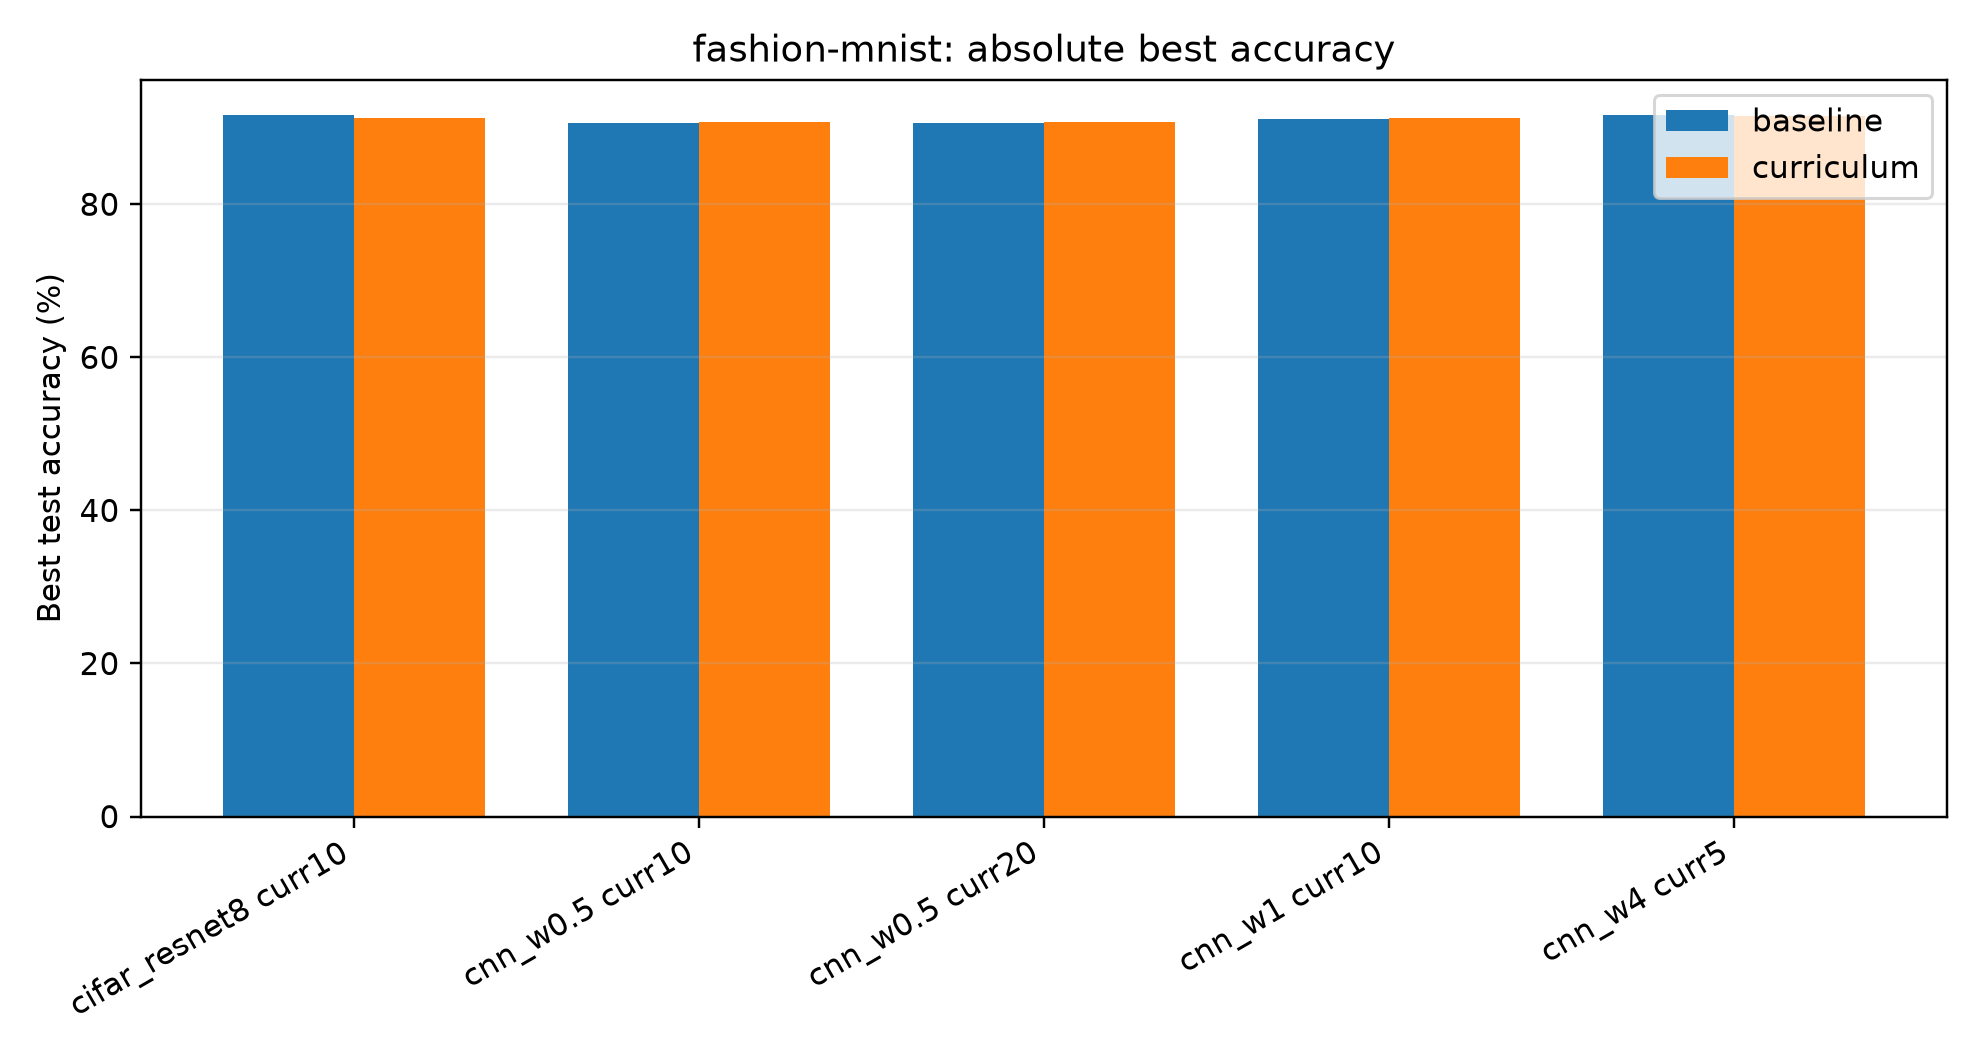
\includegraphics[width=0.82\textwidth]{figures/roughness_followup_updated_fashionmnist_absolute_best_acc.png}
    \caption{Fashion-MNIST absolute best test accuracy. Baselines are already
    high, and curriculum does not add meaningful benefit.}
    \label{fig:roughness-updated-fashionmnist-absolute}
\end{figure}

\section{CIFAR-10 control}

CIFAR-10 was added as a natural-image 10-class control. Unlike Fashion-MNIST, it
shares the image domain of CIFAR-100, but the class count is much smaller and the
automatically generated hierarchy is necessarily shallow. The tested pairs were
\texttt{cnn\_w0.5}/\texttt{curr10}, \texttt{cnn\_w0.5}/\texttt{curr20}, and
\texttt{cifar\_resnet8}/\texttt{curr10}. Results are shown in
Table~\ref{tab:roughness-cifar10-results}.

\begin{table}[h]
\centering
\small
\begin{tabular}{lrrrrr}
\hline
Model & Curriculum & Base best & Curr best & Gain & AUC gain \\
\hline
\texttt{cnn\_w0.5} & \texttt{curr10} & 0.6964 & 0.6988 & +0.24 & -2.80 \\
\texttt{cnn\_w0.5} & \texttt{curr20} & 0.6964 & 0.7042 & +0.78 & -6.75 \\
\texttt{cifar\_resnet8} & \texttt{curr10} & 0.8427 & 0.8436 & +0.09 & -3.61 \\
\hline
\end{tabular}
\caption{CIFAR-10 control results. Absolute best test accuracies are means over
seeds 42, 43, and 44.}
\label{tab:roughness-cifar10-results}
\end{table}

CIFAR-10 gives a small positive result for the weakest CNN, especially for
\texttt{curr20}, but the improvement is much smaller than on CIFAR-100 and comes
with a large AUC penalty. The CIFAR ResNet result is essentially neutral. This
places CIFAR-10 between CIFAR-100 and Fashion-MNIST: there is a small possible
benefit for a weak natural-image CNN, but the effect is not large enough to
change the main conclusion.

\begin{figure}[h]
    \centering
    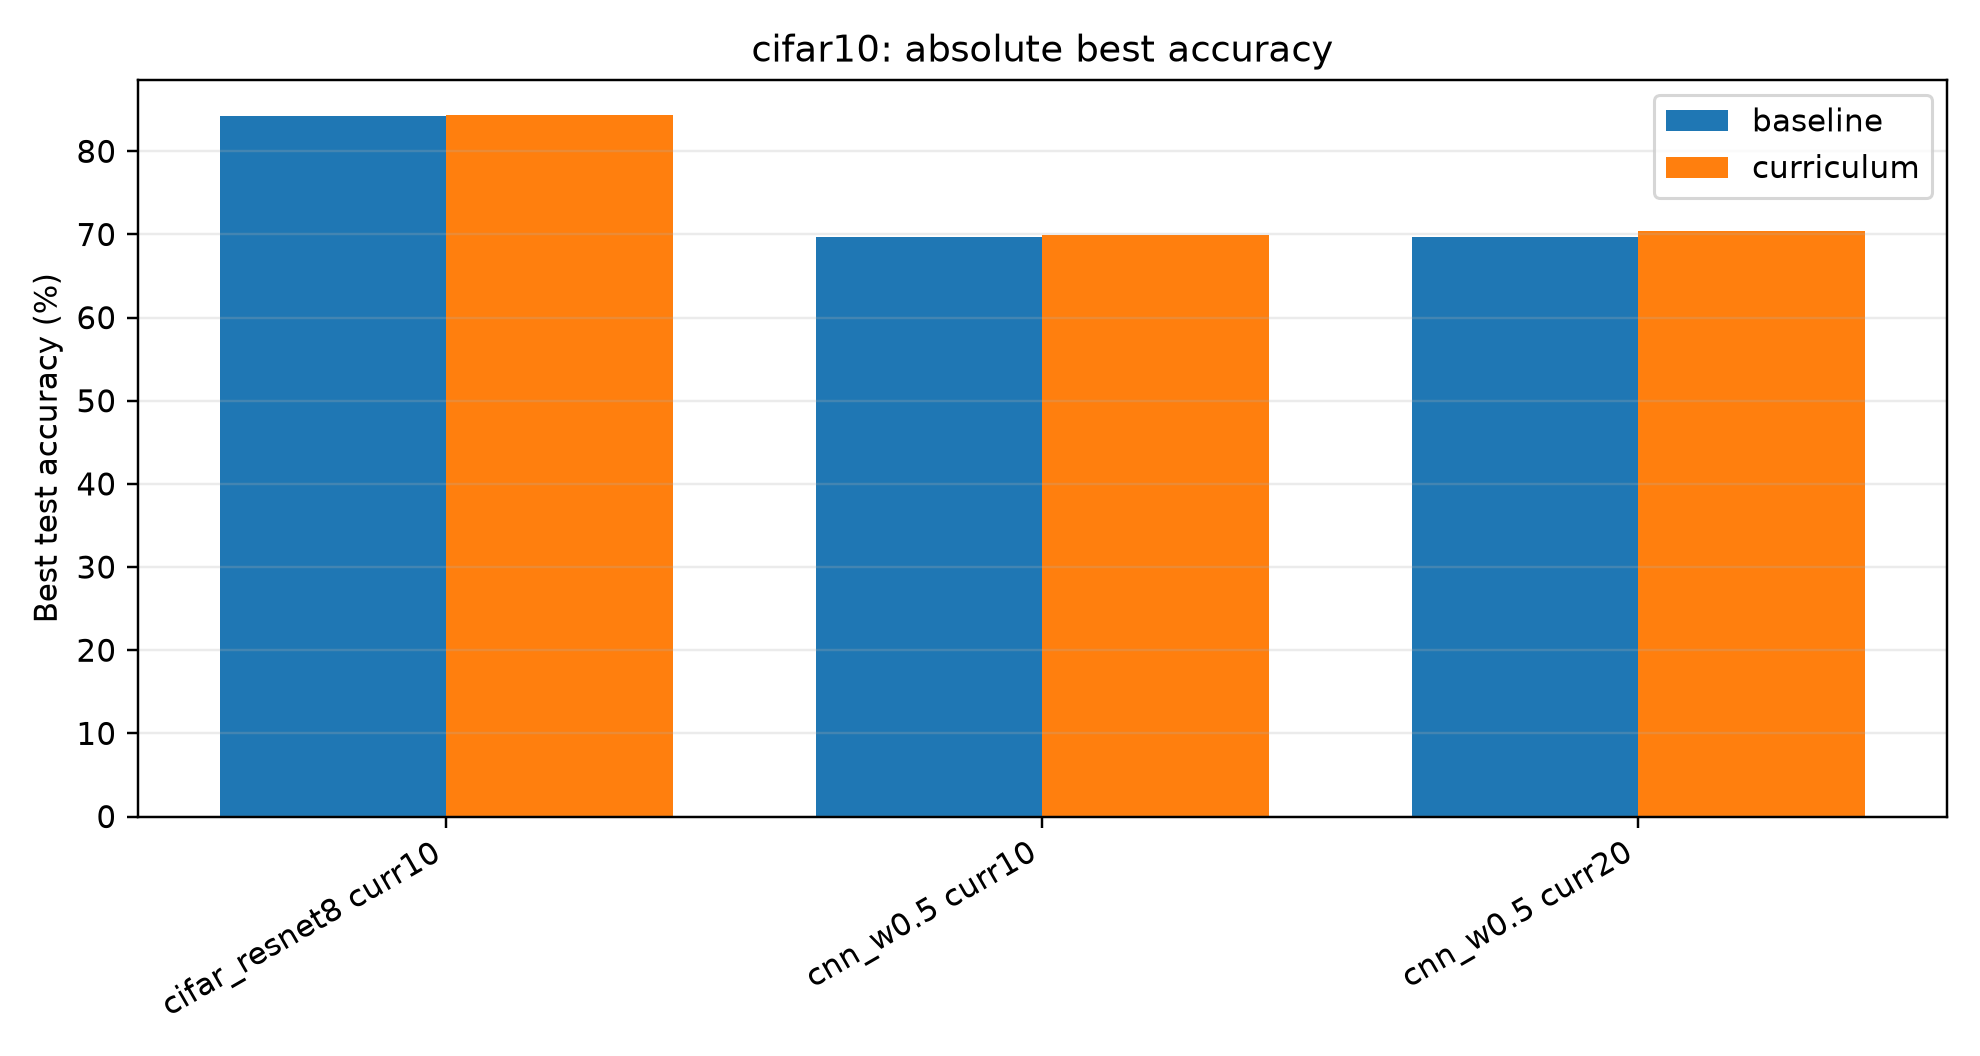
\includegraphics[width=0.82\textwidth]{figures/roughness_followup_updated_cifar10_absolute_best_acc.png}
    \caption{CIFAR-10 absolute best test accuracy for baseline and curriculum
    runs.}
    \label{fig:roughness-updated-cifar10-absolute}
\end{figure}

\begin{figure}[h]
    \centering
    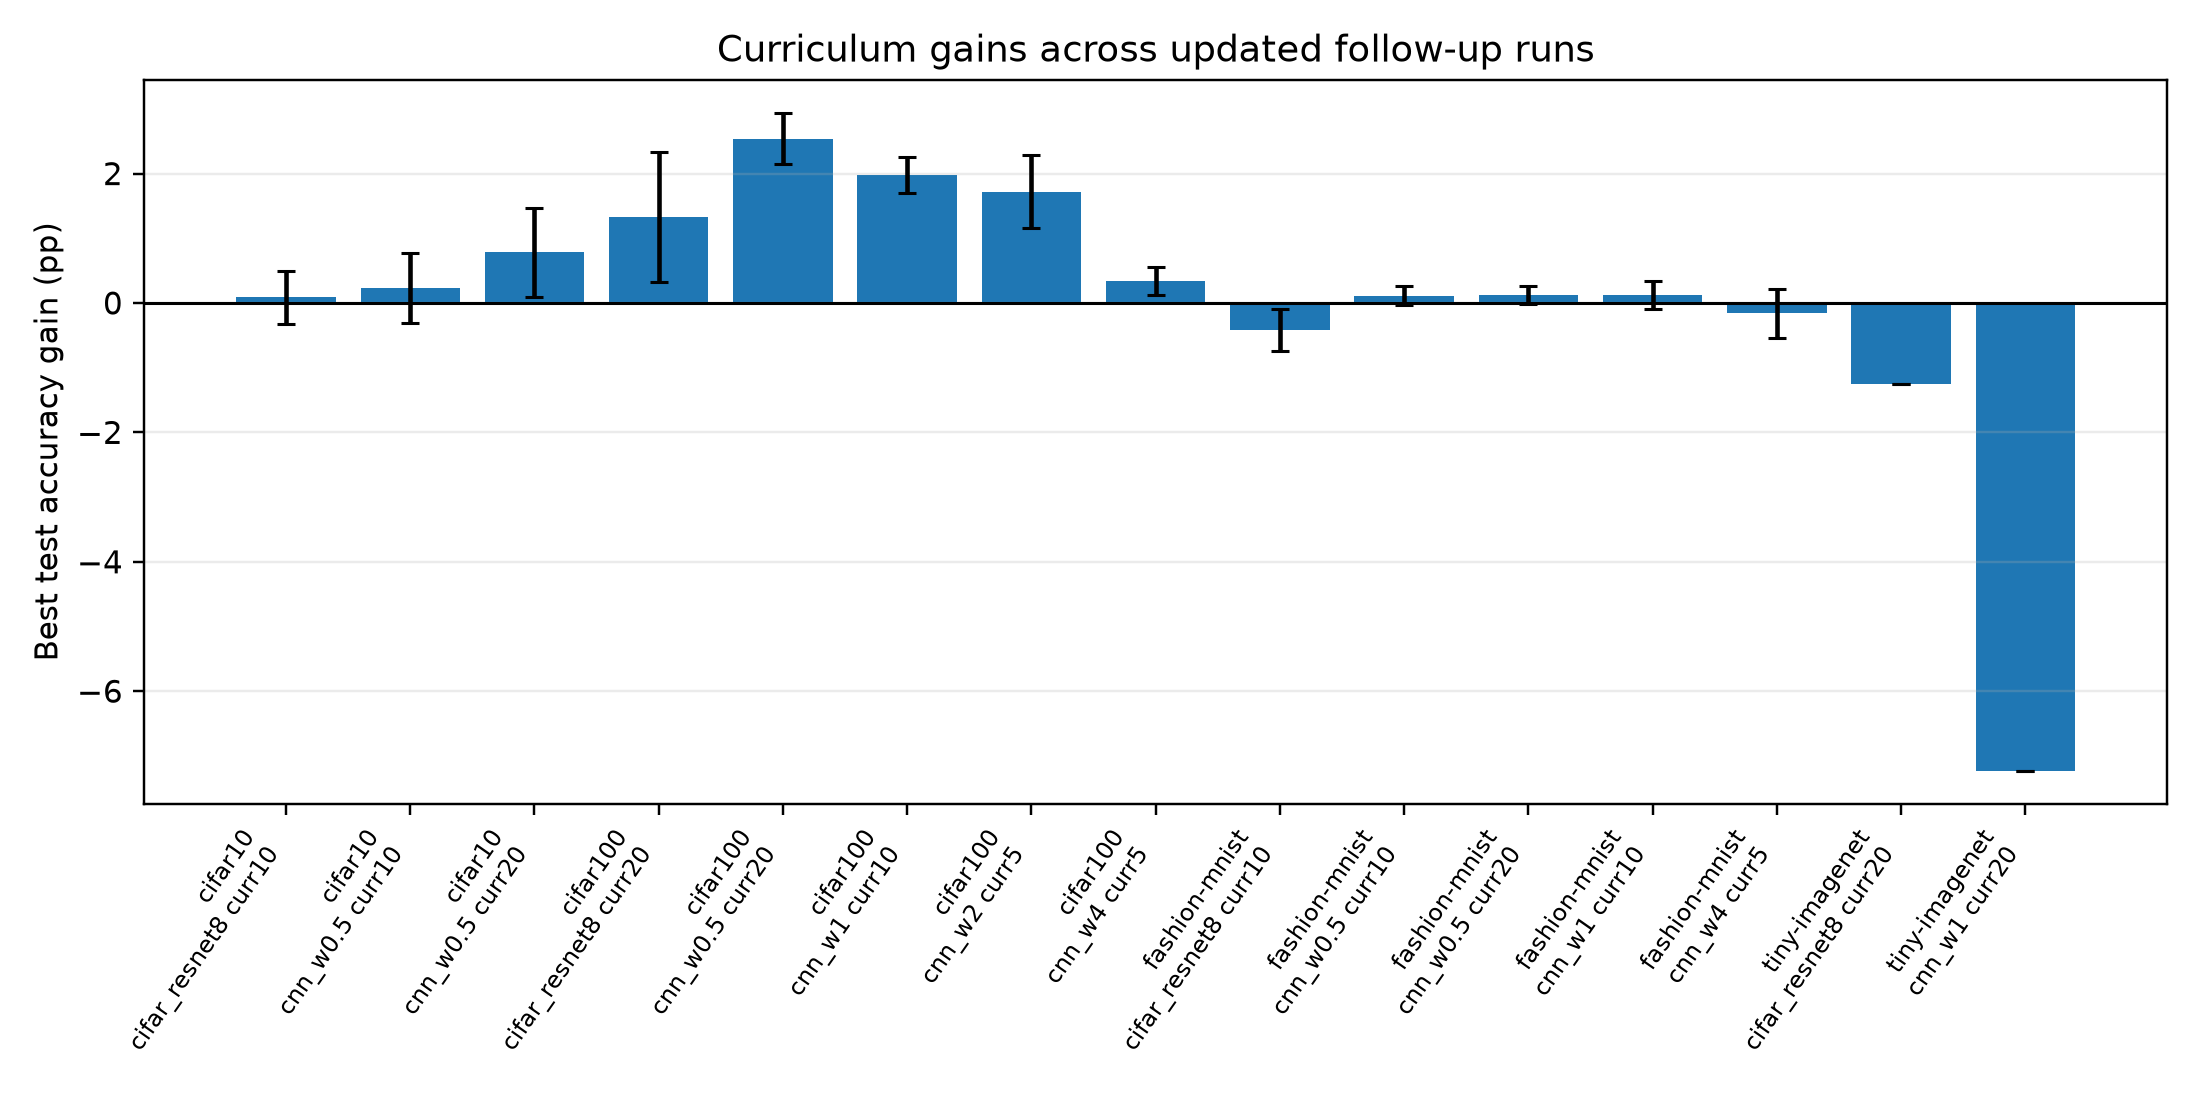
\includegraphics[width=0.95\textwidth]{figures/roughness_followup_updated_all_datasets_best_acc_gains.png}
    \caption{Updated best-test-accuracy gains across CIFAR-100, Fashion-MNIST,
    CIFAR-10, and the Tiny ImageNet pilot.}
    \label{fig:roughness-updated-all-gains}
\end{figure}

\section{Tiny ImageNet pilot}

The minimal Tiny ImageNet pilot used one seed and the pairs
\texttt{cnn\_w1}/\texttt{curr20} and \texttt{cifar\_resnet8}/\texttt{curr20}.
The results are shown in Table~\ref{tab:roughness-tinyimagenet-results}.

\begin{table}[h]
\centering
\small
\begin{tabular}{lrrrrr}
\hline
Model & Curriculum & Base best & Curr best & Gain & AUC gain \\
\hline
\texttt{cnn\_w1} & \texttt{curr20} & 0.2498 & 0.1775 & -7.23 & -5.71 \\
\texttt{cifar\_resnet8} & \texttt{curr20} & 0.3842 & 0.3716 & -1.26 & -5.52 \\
\hline
\end{tabular}
\caption{Tiny ImageNet pilot results. These are one-seed results and should be
interpreted as a stress test rather than a definitive dataset-level conclusion.}
\label{tab:roughness-tinyimagenet-results}
\end{table}

This pilot does not support direct transfer of the CIFAR-100 schedule. The
curriculum hurts both tested models. The most likely explanations are that these
models are too weak for Tiny ImageNet, the generated hierarchy is not good
enough, the curriculum is too long or too hard, or the optimizer/schedule needs
separate tuning. These results should therefore be reported as a negative pilot,
not as a final statement about Tiny ImageNet.

\section{Roughness and sharpness diagnostics}

Table~\ref{tab:roughness-ratios-updated} summarizes selected roughness ratios.
The values are \(\log_{10}(\text{curriculum}/\text{baseline})\), so negative
values mean lower roughness under curriculum and positive values mean higher
roughness.

\begin{table}[h]
\centering
\small
\begin{tabular}{llrr}
\hline
Dataset & Model/curriculum & Final sharp. & Final Hess. \\
\hline
CIFAR-100 & \texttt{cnn\_w0.5}/\texttt{curr20} & +0.03 & +0.03 \\
CIFAR-100 & \texttt{cnn\_w1}/\texttt{curr10} & +0.35 & +0.04 \\
CIFAR-100 & \texttt{cnn\_w2}/\texttt{curr5} & -0.08 & +0.06 \\
CIFAR-100 & \texttt{cnn\_w4}/\texttt{curr5} & +0.15 & +0.23 \\
CIFAR-100 & \texttt{cifar\_resnet8}/\texttt{curr20} & -0.16 & -0.30 \\
Fashion-MNIST & \texttt{cnn\_w0.5}/\texttt{curr20} & -0.10 & -0.41 \\
CIFAR-10 & \texttt{cnn\_w0.5}/\texttt{curr20} & +0.12 & +0.19 \\
Tiny ImageNet & \texttt{cnn\_w1}/\texttt{curr20} & +0.08 & +0.20 \\
\hline
\end{tabular}
\caption{Selected roughness log-ratios. Negative values indicate lower final
roughness under curriculum.}
\label{tab:roughness-ratios-updated}
\end{table}

The roughness results remain mixed after the added runs. The cleanest support
for a flattening interpretation is still CIFAR-100 \texttt{cifar\_resnet8}, where
curriculum improves accuracy and lowers both final sharpness and Hessian
estimates. The CNNs do not show a universal pattern. For example,
\texttt{cnn\_w0.5} and \texttt{cnn\_w1} improve on CIFAR-100, but their final
roughness is not consistently lower. This means the thesis should not claim that
coarse-to-fine curriculum works by always finding flatter minima.

The safer interpretation is that curriculum changes the optimization trajectory
and can improve the best solution found for some lower-capacity models. The
roughness probes are useful diagnostics, but they do not yet identify one simple
causal mechanism.

\section{Learned hierarchy inspection}

The new runs save a readable hierarchy file, \texttt{hierarchy.md}, as a W\&B
artifact. For example, a Fashion-MNIST curriculum run stores the generated
clusters under a path like:

\begin{verbatim}
/runpod-workspace/runs/<run_id>/fashion-mnist_cnn_curriculum/hierarchy.md
\end{verbatim}

and uploads the same file to W\&B artifacts. The same files were also exported
locally under:

\begin{verbatim}
thesis/appendices/hierarchies/
\end{verbatim}

The hierarchy is generated from the baseline classifier-weight distance matrix,
not from official semantic labels. Therefore it should be interpreted as the
model's learned similarity structure, rather than as a ground-truth taxonomy.
Tables~\ref{tab:hier-fashionmnist}, \ref{tab:hier-cifar10-cnn}, and
\ref{tab:hier-cifar10-resnet8} show representative learned hierarchies from seed
42. For these 10-class datasets the hierarchy has only one non-trivial coarse
level plus the singleton fine-label level.

\begin{table}[h]
\centering
\small
\begin{tabular}{lp{0.72\textwidth}}
\hline
Cluster & Fashion-MNIST \texttt{cnn\_w0.5}, seed 42, \texttt{curr20} \\
\hline
1 & \texttt{t-shirt\_top}, \texttt{trouser}, \texttt{coat}, \texttt{sandal}, \texttt{bag} \\
2 & \texttt{pullover}, \texttt{shirt}, \texttt{sneaker} \\
3 & \texttt{ankle\_boot}, \texttt{dress} \\
\hline
\end{tabular}
\caption{Representative Fashion-MNIST learned hierarchy. The grouping is only
partly semantic, which helps explain why curriculum did not provide a meaningful
benefit on this dataset.}
\label{tab:hier-fashionmnist}
\end{table}

\begin{table}[h]
\centering
\small
\begin{tabular}{lp{0.72\textwidth}}
\hline
Cluster & CIFAR-10 \texttt{cnn\_w0.5}, seed 42, \texttt{curr20} \\
\hline
1 & \texttt{airplane}, \texttt{bird}, \texttt{deer}, \texttt{horse}, \texttt{ship} \\
2 & \texttt{automobile}, \texttt{truck} \\
3 & \texttt{cat}, \texttt{dog}, \texttt{frog} \\
\hline
\end{tabular}
\caption{Representative CIFAR-10 hierarchy learned from a weak CNN baseline.
Some clusters are intuitive, for example vehicles and animals, but the hierarchy
is necessarily shallow because CIFAR-10 has only ten classes.}
\label{tab:hier-cifar10-cnn}
\end{table}

\begin{table}[h]
\centering
\small
\begin{tabular}{lp{0.72\textwidth}}
\hline
Cluster & CIFAR-10 \texttt{cifar\_resnet8}, seed 42, \texttt{curr10} \\
\hline
1 & \texttt{airplane}, \texttt{bird}, \texttt{deer} \\
2 & \texttt{ship}, \texttt{automobile}, \texttt{truck}, \texttt{frog} \\
3 & \texttt{cat}, \texttt{dog}, \texttt{horse} \\
\hline
\end{tabular}
\caption{Representative CIFAR-10 hierarchy learned from a CIFAR-style ResNet-8
baseline. The grouping differs from the CNN hierarchy, showing that the
curriculum depends on the reference model as well as the dataset.}
\label{tab:hier-cifar10-resnet8}
\end{table}

For CIFAR-100 the hierarchy is too large to print in full, but the top level of
the \texttt{cnn\_w0.5}, seed 42 hierarchy is shown in
Table~\ref{tab:hier-cifar100-top}. The complete exported Markdown and JSON files
are included in \texttt{thesis/appendices/hierarchies/}.

\begin{table}[h]
\centering
\scriptsize
\begin{tabular}{lp{0.78\textwidth}}
\hline
Cluster & CIFAR-100 top-level classes, \texttt{cnn\_w0.5}, seed 42, \texttt{curr20} \\
\hline
1 & \texttt{apple}, \texttt{sweet\_pepper}, \texttt{orange}, \texttt{pear}, \texttt{butterfly}, \texttt{possum}, \texttt{squirrel} \\
2 & \texttt{aquarium\_fish}, \texttt{train}, \texttt{lawn\_mower}, \texttt{bridge}, \texttt{bus}, \texttt{lobster}, \texttt{skyscraper}, \texttt{streetcar}, \texttt{chair}, \texttt{chimpanzee}, \texttt{cloud}, \texttt{tractor}, \texttt{pickup\_truck}, \texttt{willow\_tree}, \texttt{forest}, \texttt{rocket}, \texttt{keyboard}, \texttt{maple\_tree}, \texttt{spider}, \texttt{oak\_tree}, \texttt{tank}, \texttt{palm\_tree}, \texttt{pine\_tree}, \texttt{shark}, \texttt{bed}, \texttt{couch}, \texttt{plain}, \texttt{road}, \texttt{sea}, \texttt{castle}, \texttt{house}, \texttt{mountain} \\
3 & \texttt{lamp}, \texttt{cup}, \texttt{telephone}, \texttt{baby}, \texttt{girl}, \texttt{woman}, \texttt{boy}, \texttt{man}, \texttt{rose}, \texttt{caterpillar}, \texttt{orchid} \\
4 & \texttt{mouse}, \texttt{shrew}, \texttt{otter}, \texttt{wolf}, \texttt{raccoon}, \texttt{bear}, \texttt{seal}, \texttt{tiger}, \texttt{skunk}, \texttt{porcupine}, \texttt{elephant}, \texttt{mushroom}, \texttt{snail}, \texttt{sunflower}, \texttt{bee}, \texttt{tulip}, \texttt{dinosaur}, \texttt{poppy}, \texttt{rabbit}, \texttt{bottle}, \texttt{fox}, \texttt{hamster}, \texttt{cattle}, \texttt{camel} \\
5 & \texttt{leopard}, \texttt{lion}, \texttt{trout}, \texttt{crocodile}, \texttt{beaver}, \texttt{ray}, \texttt{turtle}, \texttt{bicycle}, \texttt{motorcycle}, \texttt{lizard}, \texttt{kangaroo}, \texttt{cockroach}, \texttt{flatfish}, \texttt{dolphin}, \texttt{whale} \\
6 & \texttt{worm}, \texttt{snake}, \texttt{can}, \texttt{table}, \texttt{television}, \texttt{bowl}, \texttt{wardrobe}, \texttt{plate}, \texttt{clock}, \texttt{crab}, \texttt{beetle} \\
\hline
\end{tabular}
\caption{Top level of the representative CIFAR-100 learned hierarchy. The
clusters contain a mixture of semantic and visually learned associations, which
is expected because the hierarchy is derived from classifier weights rather than
human labels.}
\label{tab:hier-cifar100-top}
\end{table}

This qualitative inspection is important because it separates two possible
failure modes: curriculum may fail because coarse labels are not useful for a
particular model, or because the generated hierarchy itself is poor. This
distinction is especially relevant for Tiny ImageNet, where the negative pilot
may reflect hierarchy quality, model capacity, or schedule choice rather than the
absence of any useful class structure.

\section{Interpretation}

The updated follow-up supports the following thesis-level conclusions.

First, CIFAR-100 remains the strongest positive case. The added
\texttt{cnn\_w0.5} runs show the largest gain in the follow-up, which reinforces
the capacity-conditioned result: the weaker CNNs benefit most from curriculum.

Second, the effect does not transfer automatically to easy 10-class datasets.
Fashion-MNIST is essentially negative, and CIFAR-10 shows only a small gain for
\texttt{cnn\_w0.5}. This suggests that both model weakness and dataset structure
matter. A weak model alone is not sufficient.

Third, the Tiny ImageNet pilot is negative under the tested settings. It should
not be used to conclude that curriculum cannot work on Tiny ImageNet, but it does
show that the CIFAR-100 schedule and generated hierarchy are not directly
plug-and-play.

Fourth, roughness and sharpness diagnostics are inconclusive as a mechanism.
Some successful curriculum runs are flatter by these probes, while others are
not. Therefore the correct claim is:

\begin{quote}
The experiments confirm a capacity- and dataset-dependent curriculum effect, but
current roughness probes do not prove that this effect is caused by consistently
finding flatter minima.
\end{quote}

This is the most defensible interpretation for the final thesis.

\chapter{Random-Hierarchy Ablation for CIFAR-100 Curriculum Learning}
\label{app:hierarchy-ablation-curriculum}

\section{Purpose}

Appendices~\ref{app:cifar100-model-size-curriculum} and
\ref{app:roughness-followup-curriculum} showed that the fixed coarse-to-fine
curriculum is most useful for the weaker CIFAR-100 CNNs. The remaining question
was whether this gain actually depends on the learned class hierarchy, or
whether it is mostly caused by reducing the number of labels during the first
training stage.

This appendix tests that point directly. The learned hierarchy is compared with
random hierarchies that preserve the same tree shape. In other words, the random
condition keeps the same number of hierarchy levels and the same cluster sizes,
but permutes which CIFAR-100 classes belong to those clusters. This makes the
comparison stricter than using an arbitrary random tree: the schedule and the
amount of label coarsening are matched, while the semantic or model-derived
class grouping is destroyed.

\section{Protocol}

The ablation uses the strongest cheap setting from the earlier appendices:
CIFAR-100, \texttt{cnn\_w0.5}, Adam with learning rate 0.001, batch size 128,
100 epochs, and a fixed 20-epoch curriculum. The learned hierarchy is built from
the baseline model's last-layer classifier-weight geometry, treating class
weight vectors as class embeddings. The random hierarchies are random
permutations of this learned hierarchy.

The experiment contains 15 finished runs:

\begin{itemize}
    \item three baselines, using seeds 42, 43, and 44,
    \item three learned-hierarchy curriculum runs, one per training seed,
    \item nine random-hierarchy curriculum runs, using three random hierarchy
          seeds for each training seed.
\end{itemize}

The main comparison is the learned hierarchy against the mean of the three
random hierarchies for the same training seed. The best random hierarchy per
seed is also reported as an optimistic diagnostic. That value answers a stronger
question: even if several random hierarchies were tried and the best one was
kept, would it match the learned hierarchy?

\section{Main result}

Table~\ref{tab:hier-ablation-aggregate} summarizes the ablation. Accuracy values
are means over training seeds and are shown as percentages. Gains are percentage
points relative to the matching baseline.

\begin{table}[h]
\centering
\small
\begin{tabular}{lrrrr}
\hline
Condition & Best acc. & Best gain & Final acc. & AUC gain \\
\hline
Baseline & 35.29 & -- & 32.01 & -- \\
Learned hierarchy & 37.53 & +2.24 & 32.75 & -3.83 \\
Random hierarchy mean & 35.81 & +0.53 & 31.75 & -5.39 \\
Best random hierarchy & 36.34 & +1.05 & -- & -- \\
\hline
\end{tabular}
\caption{CIFAR-100 \texttt{cnn\_w0.5} hierarchy ablation. The random mean first
averages the three random hierarchies within each training seed and then
averages across seeds. AUC is computed over the test-accuracy trajectory.}
\label{tab:hier-ablation-aggregate}
\end{table}

The learned hierarchy clearly outperforms the random hierarchy control. It
improves best test accuracy by +2.24 percentage points, while the average random
hierarchy improves it by only +0.53 points. The learned hierarchy beats the
random mean for all three training seeds. Even the best of the three random
hierarchies per seed reaches only +1.05 points on average, still well below the
learned hierarchy.

This means that the curriculum benefit is not explained only by reducing the
number of labels during early training. Random coarsening can give a small gain,
so the reduced-label effect is real, but most of the improvement in this setting
comes from using a class grouping aligned with the trained model's classifier
geometry.

\begin{figure}[h]
    \centering
    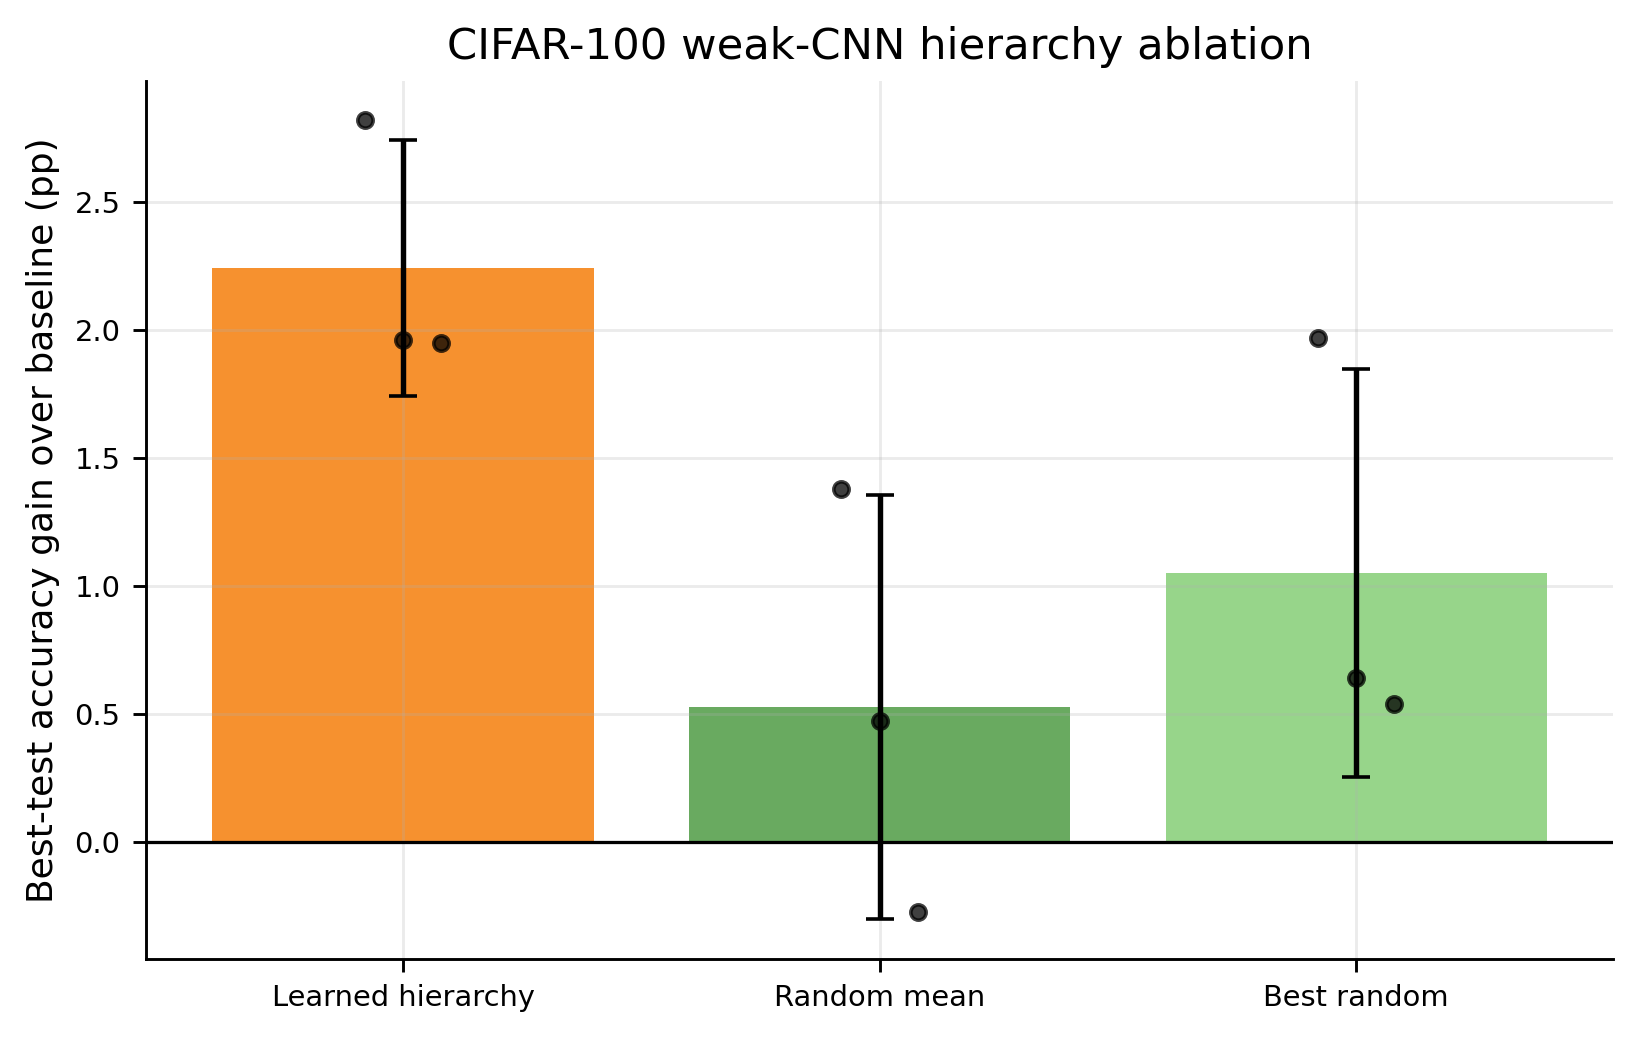
\includegraphics[width=0.82\textwidth]{figures/hierarchy_ablation_gain_comparison.png}
    \caption{Best test-accuracy gain over the matching baseline for learned and
    random hierarchies. Black points show the three training seeds. The learned
    hierarchy beats both the random mean and the best-of-three random diagnostic.}
    \label{fig:hier-ablation-gain-comparison}
\end{figure}

\section{Per-seed behavior}

Table~\ref{tab:hier-ablation-seeds} gives the paired seed-level results. The
learned hierarchy is consistently better than the random mean. The gap is
smallest for seed 42 and largest for seed 44, where the random mean is slightly
worse than the baseline.

\begin{table}[h]
\centering
\small
\begin{tabular}{rrrrrr}
\hline
Seed & Baseline & Learned & Random mean & Best random & Learned - random \\
\hline
42 & 34.98 & 37.80 & 36.36 & 36.95 & +1.44 \\
43 & 35.42 & 37.38 & 35.89 & 36.06 & +1.49 \\
44 & 35.46 & 37.41 & 35.19 & 36.00 & +2.22 \\
\hline
Mean & 35.29 & 37.53 & 35.81 & 36.34 & +1.72 \\
\hline
\end{tabular}
\caption{Seed-level best test accuracy for the hierarchy ablation. All values
except the last column are percentages. The last column is the learned-hierarchy
advantage over the random-hierarchy mean in percentage points.}
\label{tab:hier-ablation-seeds}
\end{table}

\section{Learning curves}

Figure~\ref{fig:hier-ablation-learning-curves} shows the test-accuracy
trajectories. The random curve is averaged within each training seed before
averaging across seeds, so the shaded region does not treat the nine random runs
as nine independent training seeds.

\begin{figure}[h]
    \centering
    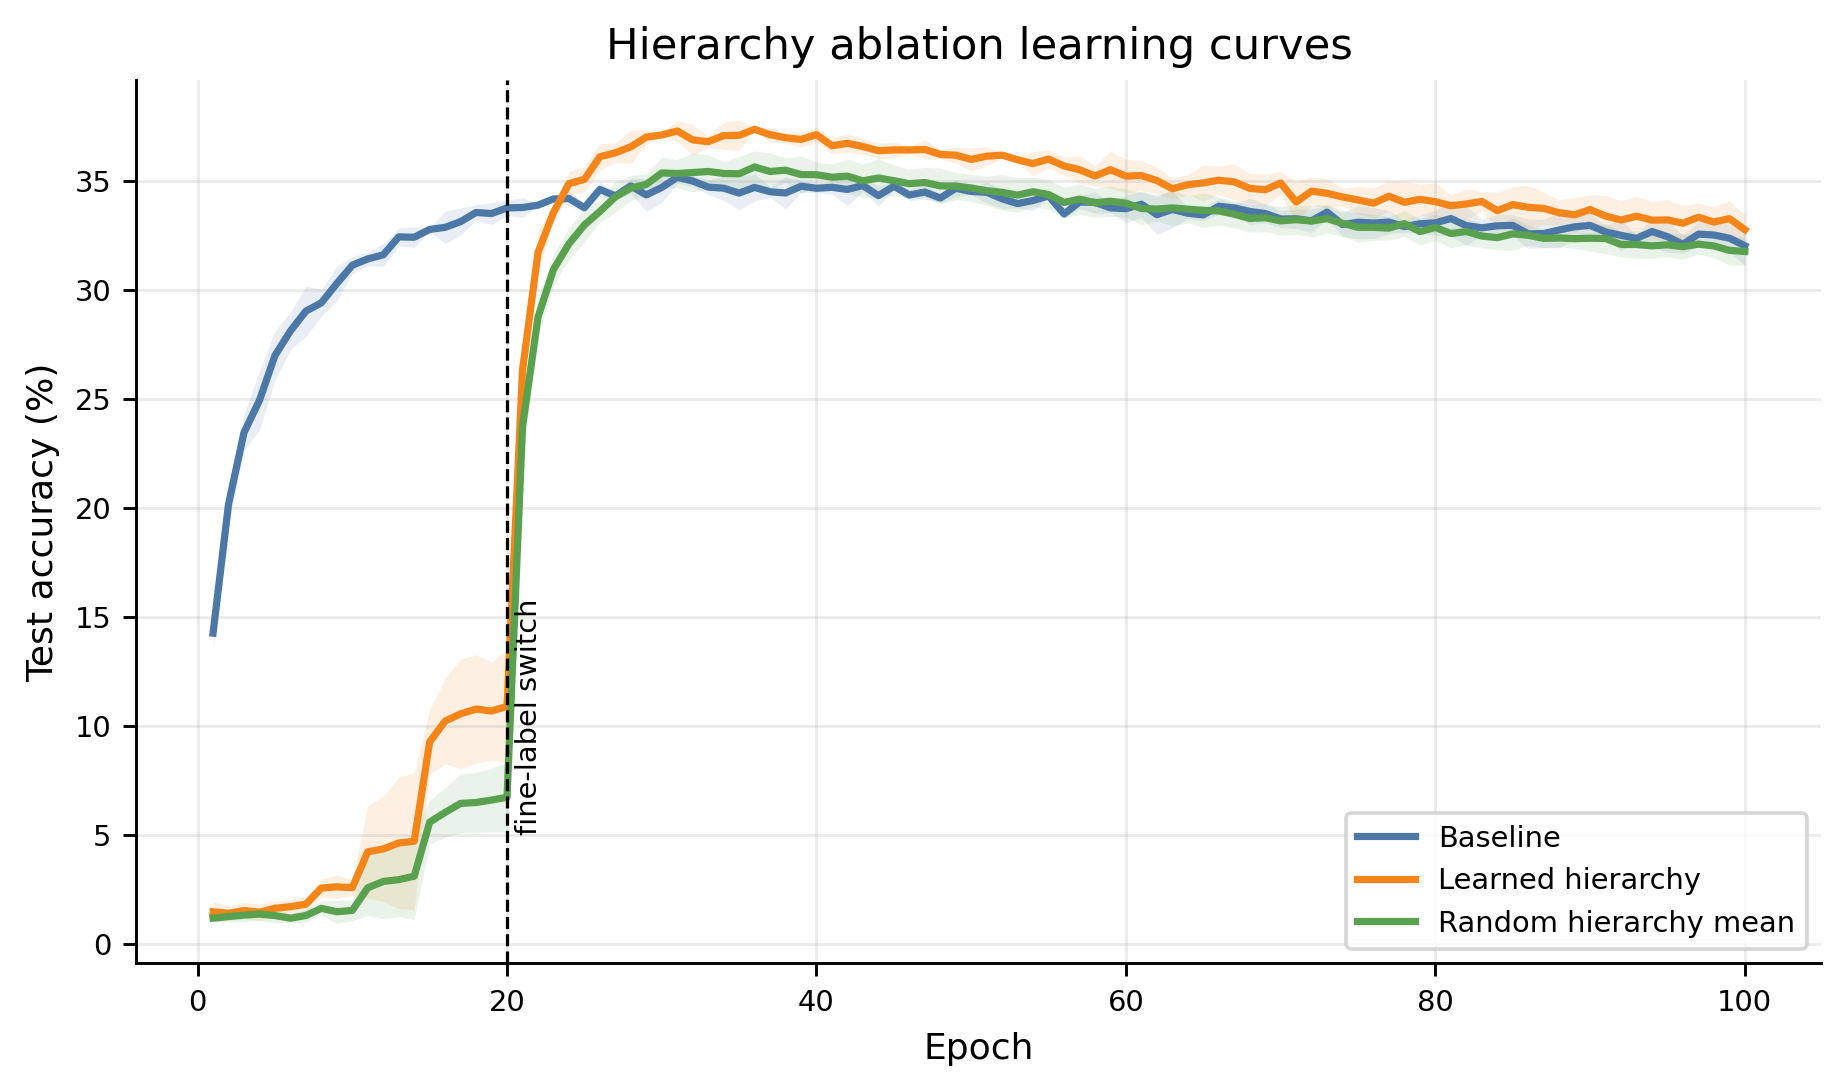
\includegraphics[width=0.90\textwidth]{figures/hierarchy_ablation_learning_curves.png}
    \caption{Learning curves for the CIFAR-100 hierarchy ablation. The vertical
    dashed line marks the switch from coarse labels to fine labels after 20
    epochs. Both curriculum variants pay an early fine-label accuracy cost, but
    the learned hierarchy recovers to a higher peak than the baseline and the
    random hierarchy.}
    \label{fig:hier-ablation-learning-curves}
\end{figure}

The trajectory confirms the interpretation from the previous appendices. The
curriculum is not a faster way to train this model: the learned-hierarchy AUC is
3.83 percentage points below baseline, and the random-hierarchy AUC is 5.39
points below baseline. The benefit is instead a higher peak after the fine-label
phase begins. The learned hierarchy provides a better warm-up than random
coarsening, while the random hierarchy mostly adds delay.

\section{Relation to the previous curriculum results}

Table~\ref{tab:hier-ablation-previous-context} places the ablation next to the
main CIFAR-100 \texttt{cnn\_w0.5} results from
Appendix~\ref{app:roughness-followup-curriculum}. The exact baselines differ
slightly because these are separate W\&B run groups, but the scale of the effect
is consistent.

\begin{table}[h]
\centering
\small
\begin{tabular}{lrrl}
\hline
Experiment/method & Best acc. & Gain & Role \\
\hline
This appendix: baseline & 35.29 & -- & ablation reference \\
This appendix: learned fixed \texttt{curr20} & 37.53 & +2.24 & hierarchy test \\
This appendix: random fixed \texttt{curr20} & 35.81 & +0.53 & random control \\
Appendix G: fixed \texttt{curr20} & 37.58 & +2.54 & previous best fixed schedule \\
Appendix G: adaptive all levels & 37.19 & +1.75 & adaptive schedule \\
Appendix G: adaptive max1 & 37.22 & +2.24 & hierarchy-depth test \\
\hline
\end{tabular}
\caption{Comparison with previous CIFAR-100 \texttt{cnn\_w0.5} results. Values
are percentages and percentage-point gains. Appendix G rows are shown for
context, not as part of the random-hierarchy ablation.}
\label{tab:hier-ablation-previous-context}
\end{table}

The ablation strengthens the earlier conclusion that hierarchy quality matters.
Appendix~\ref{app:roughness-followup-curriculum} showed that hierarchy depth and
schedule length matter; this appendix shows that the class grouping itself also
matters. The learned hierarchy is not merely a convenient way to create fewer
labels. Its grouping carries useful information for the curriculum.

\section{Conclusion}

For the strongest CIFAR-100 weak-CNN setting, the generated classifier-weight
hierarchy explains most of the curriculum gain. Random hierarchies with matched
cluster sizes give only a small improvement and remain below the learned
hierarchy even under a best-of-three random diagnostic. This does not prove that
the classifier-weight hierarchy is optimal, and it does not test all datasets or
architectures. It does, however, close the main missing ablation from
Appendix~\ref{app:roughness-followup-curriculum}: the positive CIFAR-100 result
is not just an artifact of training first on fewer labels.


\ppcolophon

\end{document}
